\documentclass [PhD] {package/uclathes}

\preamble
\frontpage
\acknowledgments
\abstract


\usepackage{Sweave}
\begin{document}

\makeintropages
\introduction

%\documentclass[12pt]{article}
%\usepackage[utf8]{inputenc}
%\usepackage{amsmath}
%\usepackage{amssymb}
%\usepackage{graphicx}
%\usepackage{tikz}
%\usepackage{hyperref}
%\usepackage{subcaption}
%\usepackage[margin=2cm]{geometry}
%\usepackage[style=authoryear, sorting=nyt, backend=bibtex, sortcites=true]{biblatex}
%\addbibresource{../../include/reference.bib}
%
%\usepackage{fullpage}
%\renewcommand{\baselinestretch}{1.25}% {1.25}
%\renewcommand{\arraystretch}{1.1}
%\renewcommand{\tabcolsep}{4pt}
%
%%% trace revision using color
%\newcommand{\reva}[1]{{\color{red} #1}}
%\newcommand{\revb}[1]{{\color{blue} #1}}
%\newcommand{\revc}[1]{{\color{cyan} #1}}
%\newcommand{\revd}[1]{{\color{blue} #1}}
%\newcommand{\reve}[1]{{\color{blue} #1}}
%%% to remove color, uncomment the following
%%\renewcommand{\reva}[1]{{#1}}  % remove color
%%\renewcommand{\revb}[1]{{#1}}
%%\renewcommand{\revc}[1]{{#1}}  % remove color
%%\renewcommand{\revd}[1]{{#1}}
%%\renewcommand{\reve}[1]{{#1}}
%
%\usepackage{amsmath,amssymb}
%\newcommand{\X}{\boldsymbol{X}}
%\newcommand{\Y}{\boldsymbol{Y}}
%\newcommand{\x}{\boldsymbol{x}}
%%\renewcommand{\u}{\boldsymbol{u}}
%\newcommand{\y}{\boldsymbol{y}}
%\newcommand{\z}{\boldsymbol{z}}
%\newcommand{\w}{\boldsymbol{w}}
%\newcommand{\R}{\boldsymbol{R}}
%\newcommand{\Rinv}{\boldsymbol{R}^{-1}}
%\newcommand{\one}{\mathbf{1}}
%\newcommand{\cov}{\textrm{Cov}}
%
%%\title{\bf A Study of Hyperparameter Tuning in a Differential Evolution Algorithm for Constructing Uniform Projection Designs}
\chapter{Tuning Differential Evolution Algorithm for Constructing Uniform Projection Designs}
%\author{Samuel Onyambu, Honquan Xu}
%\date{}
%\begin{document}
%
%\maketitle
%\begin{abstract}
%Differential Evolution (DE) is a powerful optimization algorithm inspired by the principles of natural evolution. It belongs to the class of evolutionary algorithms and has gained popularity for its simplicity, robustness, and effectiveness in solving complex optimization problems. As it works with continuous data, it has to be modified in order to work with discrete data such as design generation. Recently, \textcite{stokes2023metaheuristic} proposed such a modified DE algorithm, yet its performance heavily depends on several hyperparameters.  We aim at understanding the surface structure of the involved hyperparameters, the importance contribution of each hyperparameter, and thereby provide a guideline on optimal hyperparameter settings under different setups. We compare different types of experimental designs and surrogate models for this purpose. We illustrate the method for constructing uniform projection designs.
%\end{abstract}
%
\section{Introduction}




Experimental design construction is a fundamental aspect of research and data-driven inquiry, aimed at organizing experimental runs to extract maximum information while minimizing resource use. By strategically selecting input combinations, well-constructed designs ensure that researchers can identify key factors, estimate model parameters, and predict responses accurately \parencite{montgomery2017design}. The primary goal is to balance efficiency and comprehensiveness, whether in exploring high-dimensional spaces, optimizing processes, or assessing system robustness. Central to this process is the notion of space-filling, where design points are distributed to capture variations across the entire experimental domain, providing a solid foundation for modeling and inference \parencite{santner2003design}.

Different design strategies address diverse experimental objectives and constraints. For instance, factorial and fractional factorial designs are widely used to study the main effects and interactions of factors systematically, while response surface designs, such as central composite and Box-Behnken designs, support optimization and curvature estimation \parencite{myers2016response}. In other cases, non-traditional approaches like space-filling designs (e.g., Latin hypercube or maximin designs) and discrepancy-based designs (e.g., maxpro or uniform designs) are preferred for high-dimensional and computational experiments \parencite{joseph2016space}. Each method offers unique strengths, and the choice depends on the experimental goals, computational resources, and the nature of the underlying system being studied. Through thoughtful design construction, researchers can ensure that their experiments are not only scientifically rigorous but also cost-effective and impactful.

 In the quest for robust experimental designs, Uniform Projection Designs (UPDs) have emerged as a powerful tool for ensuring uniformity across all low-dimensional projections of the design space \parencite{sun2019uniform}. UPDs, introduced by \textcite{sun2019uniform}, are specialized space-filling designs characterized by robust performance across various design criteria and impressive space-filling properties in multiple dimensions. These designs are particularly valuable in high-dimensional settings where relationships between subsets of factors often carry critical information. However, existing algorithms for generating UPDs remain underexplored, highlighting an important area for further research. To construct UPDs, we leverage the use of Differential Evolution (DE)%, an evolutionary population-based optimization algorithm, which offers a flexible and efficient approach. DE iteratively refines candidate solutions by simulating evolutionary processes like mutation, crossover, and selection (Storn & Price, 1997). By leveraging the ability of DE to handle complex, multimodal objective functions, researchers can optimize projection-based uniformity criteria, such as minimizing the discrepancy in all subspaces. This approach provides a systematic way to generate designs that balance space-filling properties across dimensions, enabling more reliable analysis and prediction in multifactor experiments.

 
%Differential Evolution (DE) is a nature-inspired optimization algorithm that mimics the process of natural selection to efficiently search for optimal solutions within large search spaces. Since its introduction in 1997, DE has gained widespread popularity and has been extensively utilized to solve complex optimization problems. Its versatility and straightforward implementation have facilitated its integration into a multitude of real-world applications, ranging from parameter tuning in machine learning algorithms to engineering design optimization and financial portfolio management. DE has consistently demonstrated its efficacy across diverse problem domains, making it a preferred choice among researchers and practitioners alike due to its adaptability to various problem structures.

%A particularly compelling application of the DE algorithm is in the realm of design generation.
Recently, \textcite{stokes2023metaheuristic} proposed a DE-based approach for constructing order-of-addition designs, showcasing its efficiency compared to other metaheuristic algorithms, such as Simulated Annealing, Threshold Accepting, Genetic Algorithms, and Particle Swarm Optimization. Inspired by their findings, we adapt and extend their modified DE algorithm for the construction of UPDs. 

The performance of the DE algorithm is significantly influenced by its hyperparameters, which dictate the learning process of the optimization \parencite{price2006differential}. An inappropriate setting of these hyperparameters can lead to suboptimal performance of the DE algorithm. While the DE algorithm proposed by \textcite{stokes2023metaheuristic} encompasses several hyperparameters, their effects remain largely unexamined. Therefore, we aim to conduct a comprehensive study of the hyperparameters to elucidate their impacts on the algorithm's performance, providing insights that could enhance its effectiveness.

The challenge of determining the optimal hyperparameter settings for any learning process has been widely studied. Two primary frameworks dominate this landscape: the model-based framework and the model-free framework. Model-based hyperparameter optimization focuses on tuning hyperparameters by approximating the true learning algorithm, while model-free methods approach the optimization problem without parametric assumptions. Relevant literature on model-based hyperparameter optimization includes works by \textcite{falkner2018bohb, hutter2011sequential, li2018hyperband, lujan2018design, mockus1978application, snoek2012practical, wu2020efficient, zoph2016neural}. In contrast, model-free frameworks encompass techniques such as manual search, grid search, random search, genetic algorithms, and orthogonal array tuning methods \parencite{liashchynskyi2019grid}.

Our approach leverages various types of designs and models to investigate the effectiveness of DE in constructing UPDs. Specifically, we aim to address three  objectives: (i) identifying useful design types in understanding the surface structure extended by the DE hyperparameters, (ii) determining the most effective models, and (iii) developing an efficient algorithm for the construction of UPDs. We employ different types of models to evaluate the performance of different designs, enabling us to visualize the response surface of the DE algorithm's hyperparameters. This framework outlines the data generation, modeling, and analysis procedures. The insights gained from our analysis provide a general guideline for optimal hyperparameter settings necessary for generating superior uniform projection designs.%The primary goal of this paper is to tune the DE algorithm for constructing UPDs through a detailed analysis of the response surface of the DE hyperparameters. This analysis involves studying how variations in hyperparameters influence the efficiency and optimality of the generated designs. By utilizing various designs to establish hyperparameter settings for DE optimization, we can identify critical factors or combinations of factors that contribute to enhanced performance. Our objective is to thoroughly explore the hyperparameter space of the DE algorithm using established designs to optimize the generation of UPDs. 
This approach is quite different from the \textcite{lujan2018design} method which used a $2^k$ factorial design with the response surface method (RSM) and ridge regression for screening to select the important factors in the data. While \textcite{lujan2018design} focuses on factor screening and selection with the traditional RSM approach, we emphasize on the comparisons of different types of designs and surrogate models in approximating the surface structure of the DE algorithm.

% \reva{(The rest can be deleted or saved for the introduction chapter)}
% In the realms of engineering, architecture, product development, and chemical mixtures, the processes of design generation and optimization are fundamental to creating innovative and efficient solutions. The designs used for the physical and computer experiments aught  to be efficient in minimizing resource use \parencite{montgomery2017design}, enhance data quality \parencite{box2005statistics}, maximize information gain \parencite{myers2016response}, optimize performance \parencite{goos2011optimal}, enhance safety, and foster innovation.

% Uniform projection designs (UPDs) are a type of space filling designs that have been shown to be robust, perform well under various design criterias, and have good space filling properties not only in two dimensions but also in all dimensions \parencite{sun2019uniform}.
% Even though advantageous, UPDs are not widely used as there is no known construction methods provided or a package to generate them. The construction of UPDs involves minimization of a given criterion. Just like any other optimization problem several meta-heuristic methods such as the Particle Swarm Optimization (PSO), Threshold Accepting (TA) algorithm , Simulated Annealing (SA), Genetic Algorithms and Differential Evolution (DE) among others could be used to tackle the task. With design construction, the data is often categorical in nature and few of these methods have been modified to carry out the optimization.  Readily available algorithm to deal with the categorical structure of the design generation process is the DE variant by \textcite{stokes2023metaheuristic}.

% Often the proposed methods involve complicated objective functions that are difficult to optimize. Most of the space filling designs are generated by optimizing a specified criterion. For example, the maximin distance design is generated by maximizing the minimum distance between any two points in the design. These optimization processes are tedious and time consuming. Methods mentioned above or other optimization methods are invoked to obtain the optimal value. For example, in the case of Maximum Projection designs \parencite{joseph2015maximum}, along with the simulated annealing algorithm, the Non-linear optimization -- NLoptr introduced by \textcite{johnson2014nlopt} is used within the MaxPro package to do the optimization. This method requires the gradient in order for the optimization to be done. In the case whereby the gradient is not provided, the method approximates the gradient using numerical methods. This by itself is computationally expensive and also unstable. In order to generate more robust designs efficiently we would employ the DE algorithm. As such, a deeper understanding of the surface structure of the DE hyperparameters is needed.


\section{Differential Evolution Algorithm}

Originating from the pioneering work of \textcite{storn1997differential}, Differential Evolution (DE) has emerged as a powerful heuristic optimization algorithm, drawing inspiration from the mechanisms of biological evolution.  To simulate survival-of-the-fittest dynamics, DE treats each candidate or agent as a chromosome made up of several genes and implements mutation and crossover procedures that allow beneficial genes to persist into future generations \parencite{storn1997differential}. DE operates on the principle of population-based search, where a set of candidate solutions evolves over successive generations towards optimal or near-optimal solutions. At its core, DE employs mutation, crossover, and selection operators to iteratively improve the quality of solutions. The algorithm's efficacy stems from its robustness, simplicity, and ability to handle non-linear, non-convex, and noisy optimization landscapes.

%Without loss of generality, we assume that we want to {maximize} a real-valued fitness function $h:\Omega\xrightarrow{}\mathbb{R}$ by finding $\pi^{*} \in \Omega$ such that \reva{$h(\pi^{*}) \ge h(\zx)$} for all $\pi \in \Omega$, where $\Omega$ is the search space with $m$ dimensions.  The search space $\Omega$ could be unconstrained like $\mathbb{R}^m$ or constrained like $[0,1]^n$ or more complicated structures.

Without loss of generality, we assume that we want to minimize a real-valued objective function $\phi$ over an $m$-dimension space $\Omega$. It has five steps

\begin{enumerate}
    \item \textbf{Genetic Representation}:
    Let $\pi_1, \ldots ,\pi_N$ be the initial population, where each agent $\pi_i = (\pi_{i1},\dots,\pi_{im})$ is randomly chosen from $\Omega$.
    \item \textbf{Mutation}:
    Mutation expands the search space of the current population.
    For each $i = 1, \ldots , N$, mutation produces a potential donor $\nu_i$ in $\Omega$ by adding the weighted difference of two agents to a third,  all randomly chosen and distinct from the target $(\pi_i)$, that is,
    \begin{equation}
        \nu_i = \pi_a + w(\pi_b - \pi_c)\\
        \label{mutation}
    \end{equation}
    where $a \neq b \neq c$ are randomly chosen three distinct numbers from $1,\dots, N$, and they are all different from $i$.
    \item \textbf{Crossover}:
    Crossover blends the current generation of agents with the population of potential donors in order to form candidates for the next generation known as trial agents. For each $i = 1,\dots, N$, one of the $m$ variables of $\nu_i$ is randomly selected to directly enter the trial agent $u_i$. In this way, one variable is forced to change so that each $u_i$ will
    certainly differ from its original target $\pi_i$. Next, with probability $pCR$, more variables are taken from $u_i$ and placed in the trial agent. Whichever variables do not take their value from the donor inherit their original value from $\pi_i$. Assuming $j_0$ is a random number from $1, \dots, m$, this process can be written as follows: for $j = 1,\dots, m,$
    $$
    \begin{aligned}
    u_{ij} = \begin{cases} \nu_{ij}& \text{with probability }pCR
    \text{ or if } j= j_0,\\ \pi_{ij}& \text{otherwise}\end{cases}
    \end{aligned}
    $$
    \item \textbf{Selection}:
    Selection creates the next generation of agents by comparing each target to its respective trial agent. The trial agent is adopted if it leads to an improvement and is discarded otherwise. For minimization problems, this process is given by,
    $$
    \pi_i = \begin{cases} u_i & \text{if } \phi(u_i) < \phi(\pi_i)\\
    \pi_i &\text{otherwise}  \end{cases}
    $$
    \item \textbf{Repeat}:
    Repeat steps 2 through 4 over many generations until a specified
    stopping condition is satisfied.
\end{enumerate}

Though quite simplistic, its ability to balance exploration and exploitation makes it ideal for solving non-linear and multimodal problems. 

Since experimental designs lie on a discrete and constrained space, we leverage the modified DE by \textcite{stokes2023metaheuristic}. This is to ensure that the resulting mutated design is feasible. The proposed method modifies the mutation step by using the swap mutation  \parencite{michalewicz2013genetic}, one of the structural mutation operators in genetic algorithm.  In this operator, two positions in a solution are randomly selected, and their values are exchanged. This maintains the feasibility of the solution by preserving its permutation structure while introducing variation to explore the search space. The swap mutation is computationally efficient and effective at diversifying the population, reducing the risk of premature convergence. The mutation step is controlled by mutation rate $pMut$ which is the probability of swapping two elements. In addition borrowing from PSO, they induced the influence of the global best solution with a probability $pGBest$. This yielded an algorithm which contained the following hyperparameters:
\begin{itemize}
    \item $NP$ - The size of the population (N). % We consider values between $[10,  100]$
    \item $itermax$ -  the maximum number of iterations/generations used. % We consider values between $[500, 1500]$
    \item $pCR$ - Probability of crossover. %We consider values between $[0.05, 0.95]$
    \item $pMut$ - Probability of mutation. %We consider values between $[0.05, 0.95]$
    \item $pGBest$ - Probability of using the global best for mutation.
  %  We consider values between $[0.05, 0.95]$
    \item $pSelf$ - Probability of using the current agent for mutation.
\end{itemize}

They proposed three different choices of the initial agent to be mutated to obtain the proposal agent. This lead to three different variants which they referred to as DE1 which uses the global best, DE2 which uses the current agent and DE3 which uses a random agent.  

Regarding the hypermarameters, the first two, $NP$ and $itermax$, determine the budget size, whereas the other four hyperparameters affect the evolution process. The hyperparameters, $pGBest$ and $pSelf$, determine the probability of using the global best and the current agent in the mutation process, respectively. There is a constraint between these two hyperparameters, that is, $pGBest + pSelf \le 1$. The question that arises is how these hyperparameters interact with each other. Also whether we can do better than the proposed fixed probabilities to obtain the better settings for the DE algorithm for design generation.

In this study, we shall consider values between $[10,  100]$ for $NP$, $[500, 1500]$ for $itermax$, and $[0.05, 0.95]$ for $pCR$, $pMut$ and $pGBest$. We fix $pSelf = (1 - pGBest)/2$ so that there is an equal chance for selecting a current agent and a random agent if the global best is not used.

\section{Designs for Hyperparameter Settings}\label{sec:DE.designs}
Various designs can be used to set the DE hyperparameters before the optimization process. As the functions optimized by DE are often complex with many local minima, one has to carefully choose the initial point for the optimization process. These initial points are determined using any of the methods discussed below. In each subsection below one method is described, and its benefits and drawbacks are discussed.


%Data was generated using various designs. These designs include the Full factorial design (FFD), Latin hypercube design (LHD), Uniform Projection design (UPD), maximin designs, maximum projection design (MaxPro), Central composite design (CCD) and  Orthogonal Array Composite Design (OACD).

\subsection*{Full factorial designs (FFD)}
Factorial designs are a research method for studying the effects of multiple independent variables on a response variable, formalized by Sir Ronald A. Fisher in the early 20th century \parencite{fisher1935}. These designs typically involve defining factors at two or three levels, forming a grid of all possible combinations, resulting in \(2^m\) or \(3^m\) observations for \(m\) factors. Figure \ref{fig:ffd} shows a $2^3$ full factorial design.

Full factorial designs sample points at the corners of a hypercube, ensuring uniform distribution across the design space. They allow for the analysis of main effects and interactions \parencite{montgomery2017design}, but can be complex and require larger sample sizes for adequate power \parencite{tabachnick2019}.

To mitigate the need for larger samples, fractional factorial designs were introduced by David John Finney \parencite{finney1945fractional}. These designs use a fraction of runs based on the sparsity-of-effects principle, focusing on main effects and lower-order interactions. They are expressed as \(2^{m-p}\) or \(3^{m-p}\), depending on the factors set as products of others. Selecting defining relations for fractional designs is essential, with criteria such as maximum resolution and minimum aberration guiding this process \parencite{wu2011experiments}.
\begin{figure}%[!ht]
\centering

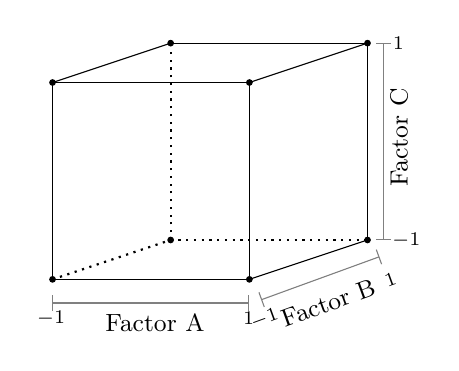
\begin{tikzpicture}
\draw[] (0,0) -- (0,2.5);
\draw[] (0,0) -- (2.5,0);
\draw[] (2.5,0) -- (2.5,2.5);
\draw[] (0,2.5) -- (2.5,2.5);
\draw[dotted, thick] (1.5, 0.5) -- (1.5, 3);
\draw[dotted, thick] (1.5, 0.5) -- (4,0.5);
\draw[] (1.5, 3) -- (4, 3);
\draw[] (4, 0.5) -- (4, 3);
\draw[dotted, thick] (0,0) -- (1.5, 0.5);
\draw[] (0, 2.5) -- (1.5, 3);
\draw[] (2.5,0) -- (4, 0.5);
\draw[] (2.5, 2.5) -- (4, 3);
\filldraw[black] (0,0) circle(1pt);
\filldraw[black] (2.5,2.5) circle(1pt);
\filldraw[black] (0,2.5) circle(1pt);
\filldraw[black] (2.5,0) circle(1pt);
\filldraw[black] (1.5,0.5) circle(1pt);
\filldraw[black] (4,0.5) circle(1pt);
\filldraw[black] (1.5,3) circle(1pt);
\filldraw[black] (4,3) circle(1pt);

\draw[gray, |-|] (-0.01,-0.3)--(2.5,-0.3);
\node[] at (-0.01, -0.5) {${}_{\text{-}1}$};
\node[] at (2.5, -0.5) {${}_1$};
\node[] at (1.3,-0.55) {\small Factor A};

\draw[gray, |-|, rotate = 20] (2.4,-1.15)--(4,-1.15);
\node[rotate = 20] at (2.7, -.5) {${}_{\text{-}1}$};
\node[rotate=20] at (4.3, 0) {${}_1$};
\node[rotate=20] at (3.5,-0.3) {\small Factor B};

\draw[gray, |-|] (4.2, 0.5)--(4.2, 3);
\node[] at (4.5, 0.5) {${}_{\text{-}1}$};
\node[] at (4.4, 3) {${}_1$};
\node[rotate=90] at (4.4, 1.8) {\small Factor C};
\end{tikzpicture}
\caption{Geometric illustration of a $2^3$ full factorial design}\label{fig:ffd}
\end{figure}

\subsection*{Central composite designs (CCDs)}
Introduced by \textcite{box1951series} as an extension of factorial designs, they were developed as a way to efficiently fit quadratic response surfaces and identify optimal process settings in industrial experiments. CCDs are full or fractional factorial designs that are augmented with two additional sets of sampling points described as ``center'' and ``axial or star'' points \parencite{box1951series}. The center point is defined by all factors being set at their center level. The CCD uses $2m$ axial points, each of which is defined by all but one factor being at their center level and the level of the remaining factor is denoted by $\alpha$, which is generally chosen to be between 1 and $\sqrt{m}$ \parencite{montgomery2017design}. The basic concepts of the CCD for $m = 2$ and $m = 3$ are depicted in Figure \ref{fig:ccd}, where the bold dots are the design points.

\begin{figure}%[!ht]
  \centering
  %\includegraphics[height=4cm,width=8cm]{images/CCD.png}

    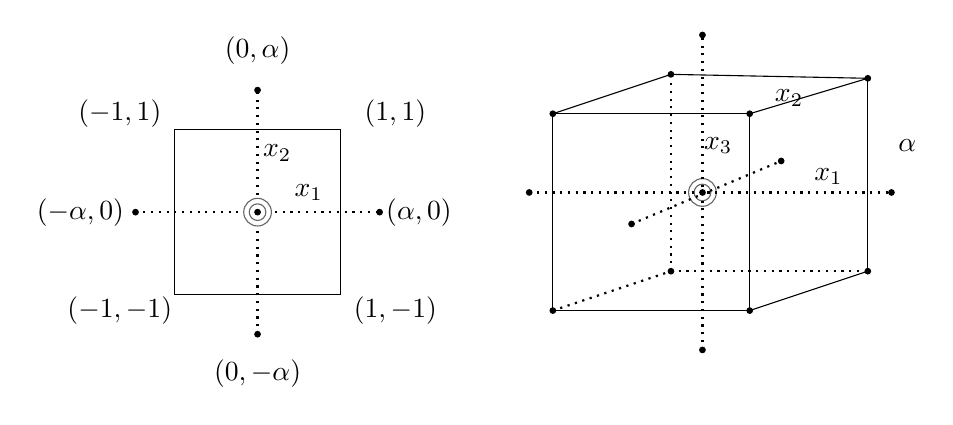
\begin{tikzpicture}
    \draw[] (5.2,0.2) -- (5.2, 2.3);
    \node[] at (4.5, 0) {$(-1,-1)$};

    \draw[] (5.2,0.2) -- (7.3,0.2);
    \node[] at (4.5, 2.5) {$(-1,1)$};

    \draw[] (7.3,0.2) -- (7.3, 2.3);
    \node[] at (8, 0) {$(1,-1)$};

    \draw[] (5.2,2.3) -- (7.3,2.3);
    \node[] at (8,2.5) {$(1,1)$};

    \node[] at (6.9,1.5) {$x_1$};
    \node[] at (6.5, 2) {$x_2$};

    \draw[dotted, thick] (4.7, 1.25) -- (7.8, 1.25);
    \filldraw[black] (4.7, 1.25) circle(1pt);
    \node[] at (4, 1.25) {$(-\alpha, 0)$};

    \filldraw[black] (7.8, 1.25) circle(1pt);
    \node[] at (8.3, 1.25) {$(\alpha, 0)$};

    \draw[dotted, thick] (6.25, -0.3) -- (6.25, 2.8);
    \filldraw[black] (6.25, -0.3) circle(1pt);
    \node[] at (6.25, -0.8) {$(0,-\alpha)$};

    \filldraw[black] (6.25, 2.8) circle(1pt);
    \node[] at (6.25, 3.3) {$(0,\alpha)$};

    \filldraw[color=black!60, fill=white](6.25,1.25) circle (5pt);
    \filldraw[color=black!60, fill=white](6.25,1.25) circle (3pt);
    \filldraw[black](6.25,1.25) circle (1pt);

    \draw[] (10,0) -- (10, 2.5);
    \draw[] (10,0) -- (12.5,0);
    \draw[] (12.5,0) -- (12.5,2.5);
    \draw[] (10,2.5) -- (12.5,2.5);
    \draw[dotted, thick] (11.5, 0.5) -- (11.5, 3);
    \draw[dotted, thick] (11.5, 0.5) -- (14,0.5);
    \draw[] (11.5, 3) -- (14, 2.95);
    \draw[] (14, 0.5) -- (14, 2.95);
    \draw[dotted, thick] (10,0) -- (11.5, 0.5);
    \draw[] (10, 2.5) -- (11.5, 3);
    \draw[] (12.5,0) -- (14, 0.5);
    \draw[] (12.5, 2.5) -- (14, 2.95);
    \filldraw[black] (10,0) circle(1pt);
    \filldraw[black] (12.5,2.5) circle(1pt);
    \filldraw[black] (10,2.5) circle(1pt);
    \filldraw[black] (12.5,0) circle(1pt);
    \filldraw[black] (11.5,0.5) circle(1pt);
    \filldraw[black] (14,0.5) circle(1pt);
    \filldraw[black] (11.5,3) circle(1pt);
    \filldraw[black] (14,2.95) circle(1pt);

    \filldraw[color=black!60, fill=white](11.9,1.5) circle (5pt);
    \filldraw[color=black!60, fill=white](11.9,1.5) circle (3pt);
    \filldraw[black](11.9,1.5) circle (1pt);

    \draw[dotted, thick] (11,1.1) -- (12.9,1.9);
    \node[] at (13,2.7) {$x_2$};
    \filldraw[black] (11,1.1) circle(1pt);
    \filldraw[black] (12.9,1.9) circle(1pt);

    \draw[dotted, thick] (9.7, 1.5) -- (14.3,1.5);
    \node[] at (13.5,1.7) {$x_1$};
    \filldraw[black] (9.7,1.5) circle(1pt);
    \filldraw[black] (14.3,1.5) circle(1pt);

    \draw[dotted, thick] (11.9, -0.5) -- (11.9, 3.5);
    \node[] at (12.1,2.1) {$x_3$};
    \filldraw[black] (11.9, -0.5) circle(1pt);
    \filldraw[black] (11.9, 3.5) circle(1pt);
    \node[] at (14.5,2.1) {$\alpha$};
    \end{tikzpicture}
  \caption{CCD for $m=2$ and $m = 3$ }\label{fig:ccd} %\parencite{ahn2015central}}
\end{figure}





%\subsection*{Orthogonal arrays (OA)} \reva{(This paragraph can be deleted?)}
%An orthogonal array is a structured arrangement of experimental runs that ensures each factor level combination occurs with equal frequency. In other words, orthogonal arrays provide a systematic way to design experiments in a balanced manner, allowing for efficient and effective exploration of multiple factors and their interactions \parencite{box1978statistics, wu2011experiments}. While the full, fractional, and central composite designs are described as ``regular'' designs because the effect of each factor is either estimated independently of all others or fully aliased with one of the other factors, orthogonal arrays are described to be ``non-regular'' as they do not possess this property \parencite{burton2022design}. In
%contrast to regular fractional factorial designs where some factorial effects are fully aliased, orthogonal array-based designs can incorporate partial aliasing which could capture the effect of all two-factor interactions using a small number of runs.
%More specifically, an orthogonal array-based design
%$O A\left(n, s_1^{m_1} s_2^{m_2} \ldots s_\gamma^{m_\gamma}, t\right)$ is one that has an $n \times m$ design matrix where $n$ is the number of runs and $m=m_1+\cdots+m_\gamma$.
%The strength of the orthogonal array $O A$ is denoted by $t$, whereby $m_i$ columns have $s_i \geq 2$ levels such that, within any $t$ columns, all possible level combinations occur equally often. Note that $\gamma=1$ corresponds to the case where all factors have the same number of levels and the associated designs are described as symmetrical orthogonal arrays. Designs that have $\gamma > 1$ are described asymmetric or mixed-level orthogonal arrays \parencite{burton2022design}.
%One advantage of OAs over regular fractional factorial designs is that the $OA$ designs are more efficient and can accommodate mixed level factors with a small number of runs \parencite{ding2013use, jaynes2016use, xu2014combining}


\subsection*{Orthogonal array composite designs (OACD)}
Introduced by \textcite{xu2014combining}, an OACD is a class of composite designs based on a two-level factorial design and a three-level {orthogonal array (OA)}. An $\mathrm{OA}$ of $n$ runs, $m$ columns, $s$ levels, and strength $t$, denoted by $\mathrm{OA}\left(n, s^m, t\right)$, is an $n \times m$ matrix in which all $s^t$ level-combinations appear equally often in every $n \times t$ submatrix \parencite{wu2011experiments}. For example, a $2^m$ factorial design can be viewed as $\operatorname{OA}\left(n, 2^m, t\right)$ with $n=2^m$ and $t=m$. Similarly, a three-level OA can be written as $\operatorname{OA}\left(n, 3^m, t\right)$. Thus, an OACD is a composite design which consists of a two-level factorial design as its factorial points, a three-level OA as its additional points, plus any number of center points \parencite{luna2022orthogonal}.

\subsection*{Space filling designs}
While the previously discussed designs utilize sampling points that are at the boundaries of the design space, space filling designs generate samples that are dispersed throughout the multidimensional design space and not just at the boundary of the design space. These designs are important in sampling a surface as they could capture important regions thereby minimizing the bias between the true structure of the surface and the estimated surface from the sampled points \parencite{gardner2006small, giunta2003overview}. They are of various types depending on the approach used to construct them, e.g., sampling-based -- Latin Hypercube designs, distance-based -- maximin designs, and distribution -- based uniform designs \parencite{burton2022design}.

\begin{description}
  \item Latin hypercube designs (LHDs) -- Based on \textcite{mckay1992latin}'s Latin hypercube sampling, it divides the range of each factor into  bins of equal size, where $n$ also corresponds to the number of samples to be generated resulting in a total of $n^m$ combinations where $m$ is the number of factors  being considered. The $n$ samples are then randomly generated such that for all one-dimensional projections, there will be only one sample in each bin.
  \item Maximin distance designs -- Introduced by \textcite{johnson1990minimax}, this design aims at spreading out the design points in the design space by maximizing the minimum  distance between any two design points. It thus tends to place a large proportion of points at the corners and on the boundaries of the design space. Mathematically, this can be formulated as follows. Suppose we want to construct an $n$-run design in $m$ factors. Let the design region be the unit hypercube $\mathcal{X}$ and let the design be $D=\left\{\x_1 \ldots, \x_n\right\}$, where each design point {$\x_{i}$} is in $\mathcal{X}=[0,1]^m$. The maximin design optimizes the function below:
$$
\max _D \min _{i \ne j} d\left(\x_i, \x_j\right),
$$
where $d\left(\x_i, \x_j\right)$ is the  distance between the points $\x_i$ and $\x_j$.
  \item Maximin Latin hypercube designs -- Unlike Latin hypercube designs,  maximin distance designs do not have good projection properties for each factor. \textcite{morris1995exploratory} proposed to overcome this problem by searching for the maximin distance design within the class of Latin hypercube designs. They also proposed to use the following criterion to achieve maximin distance:
\begin{equation}
\min _D\left\{\sum_{i=1}^{n-1} \sum_{j=i+1}^n \frac{1}{d^p\left(\x_i, \x_j\right)}\right\}^{1 / p}
\label{morris_mitchelle}
\end{equation}
where $p > 0$ is chosen large enough, say $p=15$.

  \item Maximum projection (MaxPro) designs  -- Although maximin Latin hypercube designs ensure good space-filling in $m$ dimensions and uniform projections in each dimension, their projection properties in two to $m - 1$ dimensions are not known. By the effect sparsity principle \parencite{wu2011experiments}, only a few factors are expected to be important. To curb this, \textcite{joseph2015maximum} proposed a different criterion:

\begin{equation}
\min _D \psi(D)=\left\{\frac{2}{n(n-1)} \sum_{i=1}^{n-1} \sum_{j=i+1}^n \frac{1}{\prod_{l=1}^m\left(x_{i l}-x_{j l}\right)^2}\right\}^{1 / m} .
\end{equation}
and showed that the design that minimizes $\psi(D)$ tends to maximize its projection capability in all subspaces of factors, and thus named these designs as maximum projection designs.
\end{description}


\section{Modeling}\label{sec:models}
We consider three different frameworks to model the data: (a) Linear Model, (b) Kriging Model and (c) Heterogeneous Gaussian Process (HetGP).

\subsection*{{Linear Model (lm)}}

For $m$ quantitative factors, denoted by $x_1, \ldots, x_m$, a second-order linear model is defined as
\begin{equation}
y=\beta_0+\sum_{i=1}^m \beta_i x_i+\sum_{i=1}^m \beta_{i i} x_i^2+\sum_{i<j} \beta_{i j} x_i x_j+\epsilon
\end{equation}
where $\beta_0, \beta_i, \beta_{i i}$, and $\beta_{i j}$ are the intercept, linear, quadratic, and bilinear (or interaction) terms, respectively, and $\epsilon$ is the error term. This model is simple and provides a straightforward way to model and understand relationships between the response variable and the factors. The main effects are easy to to interpret.  % In R the $lm$ function was used to fit this model.

\subsection*{Kriging Model (km)}
Proposed by South African geostatistician \textcite{krige1951statistical}, Kriging is one of the methods used to interpolate intermediate values, whereby these intermediate values are modeled using Gaussian Process (GP) which is governed by prior co-variances. It provides a probabilistic prediction of the output variable, as well as an estimate of the uncertainty of the prediction \parencite{chevalier2014kriginv}. The kriging predictors interpolating the observations are assumed to be noise-free \parencite{roustant2012dicekriging}. Intermediate interpolated values obtained by Kriging are the best linear unbiased predictors. % There are two forms of fitting a kriging model:  Simple Kriging and Universal Kriging.

%\reva{(not helpful to talk about simple kriging.)}
%\iffalse %
%In simple kriging (SK), $Y(\x)$ is assumed to be the sum of a known deterministic trend function and a centered square-integrable process:
% \begin{equation}
%       Y(\x) = \mu(\x) + Z(\x),
% \end{equation}
% where \(\mu(\x)\) is the trend function and \(Z(\x)\) is a stationary GP with zero mean and covariance function \(\psi\). % that is known %and \(\epsilon \sim N(0,\tau^2)\) is a random error term independent of \(Z(x)\).
% In Universal Kriging (UK), the trend $\mu(\x)$ is known up to a set of linear trend and unknown coefficients. This linear trend is set to be the linear combination of some fixed basis functions $f_i$'s.
% That is
% \begin{equation}
% \mu(\x)=\sum_{i=1}^k \beta_i f_i(\x) .
% \end{equation}\\
% UK consists of deriving the best linear predictions of $Y(\x)$ based on the observations
% while estimating the vector $\beta:=(\beta_1, \dots,\beta_k)^\top$ on the fly. Note that in the specific case where the basis functions reduce to a unique constant function, UK is referred to as ordinary Kriging (OK) \parencite{roustant2012dicekriging}.
% \fi

The Kriging model consists of two parts: a trend and a GP. The trend part is often modeled as a regression on some fixed basis functions. In the specific case where the basis functions reduce to a constant function, it is referred to as ordinary Kriging  \parencite{roustant2012dicekriging}. The general form is as given below
\begin{equation}\label{eq:UK}
      Y(\x) = \sum_{i=1}^k \beta_i f_i(\x) + Z(\x),
\end{equation}
where $f_1, \ldots, f_k$ are $k$ basis functions, $\beta_1, \dots,\beta_k$ are corresponding regression coefficients, and  \(Z(\x)\) is a stationary GP with zero mean and covariance function \(\psi\). % that is known %and \(\epsilon \sim N(0
The covariance function $\psi$ completely defines the behavior of the Gaussian Process $Z(\x)$. It is defined as
\begin{equation}
%\resizebox{0.5\textwidth}{!}{$
\psi\left(\x_{i},\x_{j}\right) =\operatorname{Cov} \left(Z\left(\x_{i}\right), Z\left(\x_{j}\right)\right) = \sigma^{2} \prod_{l=1}^{m} K\left(h_{l} ; \theta_{l}\right),
%$}
\end{equation}
where $\sigma^2$ is the scale parameter called the process variance,
$h_l = |x_{i,l}-x_{j,l}|$, $x_{i,l}$ and $x_{j,l}$ are the $l$th elements of the $i^{th}$ run $\x_i$ and the $j^{th}$ run $\x_j$, and $K(h ; \theta)$ is the correlation function.
%For a stationary GP, the mean and covariance remain constant with respect to time.
The parameters $\theta_l$ chosen for the correlation function $K\left(h_{l};\theta_{l}\right)$  must be positive. Otherwise the correlation function will not be feasible. These parameters are chosen to be physically interpretable in the same unit as the corresponding variables. They are often referred to as the \textit{characteristic length-scales} by \textcite{rasmussen2006gaussian}. Popular correlation functions include Gaussian, Mat\'ern, and power-exponential family correlation functions. The Mat\'ern function with parameter $\nu = 5/2$ is often chosen as the default when fitting kriging models. It is defined as:
\begin{equation}
K(h ; \theta)=\left(1+\frac{\sqrt{5} h}{\theta}+\frac{5 h^{2}}{3 \theta^{2}}\right) \exp \left(-\frac{\sqrt{5} h}{\theta}\right).
\end{equation}
The unknown parameters can be estimated via MLE or cross validation. In R, the \texttt{km} function  in the DiceKriging package was used to fit the kriging model.


\subsection*{{Heteroskedastic Gaussian Process (HetGP)}}

HetGP follows the simplifying assumption in the computer experiments literature in using a mean zero GP, which shifts all of the modeling effort to the covariance structure \parencite{binois2018practical}.
Observation model is given by %\reva{(provide more details on hetGP. what is $r(x)$?)}
\begin{equation}
y_i = y\left(\x_i\right)=f\left(\x_i\right)+\varepsilon_i, \quad\varepsilon_i \sim \mathcal{N}\left(0, r\left(\x_i\right)\right),
\end{equation}
where $f(\x_i)$ is a GP with covariance or kernel $k(\cdot, \cdot)$ and $r(\x_i)$ is the variance of $\epsilon_i$ which depends on $\x_i$. The  kernel $k(\cdot, \cdot)$ is positive definite, with parameterized families such as the Gaussian or Mat\'ern being typical choices. If $r(\x_i)=\tau^2$ is a constant, then the process is homoskedastic.
In matrix notation, the modeling framework just described is equivalent to writing
$$
Y \sim \mathcal{N}\left(\mathbf{0}, \mathbf{K}_n+\boldsymbol{\Sigma}_n\right),
$$
where $\mathbf{K}_n$ is the $n \times n$ matrix with $(i, j)$ coordinate $k\left(\x_i, \x_j\right)$, and $\boldsymbol{\Sigma}_n=\operatorname{Diag}\left(r\left(\x_1\right), \ldots, r\left(\x_n\right)\right)$ is the variance matrix of the  vector of independent noise $\varepsilon_i$.

Given the kernel function $k(\cdot, \cdot)$ and data $\y=(y_1,\ldots,y_n)^{\top}$, multivariate normal (MVN) conditional identities provide a predictive distribution at site $\x: Y(\x) \mid \y$, which is Gaussian with parameters
$$
\begin{aligned}
\mu(\x) & =\mathbb{E}(Y(\x) \mid \y)=\mathbf{k}(\x)^{\top}\left(\mathbf{K}_n+\mathbf{\Sigma}_n\right)^{-1} \y,  \\
\sigma^2(\x) & =\mathbb{V} \operatorname{ar}(Y(\x) \mid \y)=k(\x, \x)+r(\x)-\mathbf{k}(\x)^{\top}\left(\mathbf{K}_n+\mathbf{\Sigma}_n\right)^{-1} \mathbf{k}(\x) ,
\end{aligned}
$$
where $\mathbf{k}(\x)=\left(k\left(\x, \x_1\right), \ldots, k\left(\x, \x_n\right)\right)^{\top}$.
In R, the \texttt{mleHetGP} function in hetGP package is used to fit this model with the default Gaussian kernel.


\section{The Data Generation Process}
%\reva{(I've made many changes in this section. Revise as needed.)}

We aim to obtain optimal DE hyperparameter settings that can be used to generate UPDs. %The objective function is the uniform projection criterion. %This is then minimized and the minimum returned as the response value.

\subsection*{The Objective Function: Uniform Projection Design Criterion}
Proposed by \textcite{sun2019uniform}, the uniform projection criterion solely focuses on  two-dimensional projections. This is due to two factor interactions being more important than three-factor or higher-order interactions. The motivating idea was that although designs with low discrepancy have good uniformity in the full-dimensional space, they can have bad projections in lower dimensional spaces, which is undesirable when only a few factors are active. Thus designs with better projection properties are preferred. \textcite{sun2019uniform} argued that the uniform projection designs scatter points uniformly in all dimensions and have good space-filling properties in terms of distance, uniformity and orthogonality.

The uniform projection design criterion is defined using the centered $L_2$-discrepancy.
For an $n \times m$ design $D=\left(x_{i k}\right)$ with $s$ levels from $\{0, 1, \ldots, s-1 \}$, its (squared) centered $L_2$-discrepancy is defined as
$$
\begin{aligned}
  \mathrm{CD}(D)= & \frac{1}{n^2} \sum_{i=1}^n \sum_{j=1}^n
  \prod_{k=1}^m\left(1+\frac{1}{2}\left|z_{i k}\right| +
  \frac{1}{2}\left|z_{j k}\right| -
  \frac{1}{2}\left|z_{i k}-z_{j k}\right|\right) \\
  & -\frac{2}{n} \sum_{i=1}^n \prod_{k=1}^m\left(1+\frac{1}{2}
  \left|z_{i k}\right|-\frac{1}{2}\left|z_{i k}\right|^2\right)+
  \left(\frac{13}{12}\right)^m,
  \end{aligned}
$$
where $z_{i k}=\left(2 x_{i k}-s+1\right) /(2 s)$. Then the uniform projection criterion is to minimize
\begin{equation}
  \phi(D)=\frac{2}{m(m-1)} \sum_{|u|=2} \mathrm{CD}\left(D_u\right),
  \label{upd}
\end{equation}
where $u$ is a subset of $\{1,2, \ldots, m\},|u|$ denotes the cardinality of $u$ and $D_u$ is the projected design of $D$ onto dimensions indexed by the elements of $u$. The $\phi(D)$ is the average centered $L_2$-discrepancy values of all two-dimensional projections of $D$.

We implemented the DE and uniform projection criterion in the package \texttt{UniPro}. % \texttt{Meta4Design}.
The following code generates an $n\times m$ UPD with $s$ levels
\begin{Schunk}
\begin{Sinput}
> UniPro(n, m, s, NP, itermax, pMut, pCR, pGBest, seed)
\end{Sinput}
\end{Schunk}
where $NP$, $itermax$, $pMut$, $pCR$ and $pGBest$ are DE hyperparameters described in Section 2, and seed is an optional seed for random number generators that ensures reproducibility.

As the task of design generation is quite complex, only 3 design sizes are considered.  A UPD of size $30\times3$ is considered as a small and easy task, $50\times5$ as a medium task and $70\times 7$ as a large and difficult task. We only consider the construction of designs with $s=n$ so that the resulting UPD is an LHD.

\subsection*{Training and testing data}

Designs discussed in Section \ref{sec:DE.designs} are used to determine the parameter settings for the DE algorithm hyperparameters. Specifically, we construct five designs: a CCD with 43 runs (\verb|ccd3_43|), an OACD with 50 runs (\verb|oacd3_50|), 50-run random LHD, 50-run maximin LHD, and 50-run maxpro LHD. All designs have five factors, one for each hyperparameter. Each run corresponds to a setting of the five hyperparameters. The CCD and OACD have 3 levels while the rest have 50 levels. The levels are linearly interpolated within the minimum and maximum factor values for each hyperparameter. Generating the test data from the $3^5$ factorial, 243-run random LHD, and the  $4^5$ factorial seems good enough. This is because the random LHD enjoys the maximum space-filling property in all one dimensions, while the $3^5$ and $4^5$ factorial designs cover the entire 5-dimensional input space in a uniform fashion. % \parencite{shi2023evaluating}.

Given the target design size $(n \times m)$ and a setting of the five hyperparameters, we run the \texttt{UniPro} function to generate an $n \times m$ UPD and the resulting $\phi(D)$ value defined in  \eqref{upd}. This is recorded as the response value for that particular hyperparameter setting and target design size. For each setting, the DE algorithm is replicated ten times yielding ten replicates for the response. These are then aggregated to obtain the mean and the standard deviation of the response.
Thus we obtain five training datasets for each target size.

%Due to the difference in the structure of the designs, various factor levels were employed, with each hyperparameter domain remaining as previously stated while the levels within the minimum and maximum factor values were linearly interpolated.

%For the training data, one of the designs amongst a CCD with 43 runs (\verb|ccd3_43|), an OACD with 50 runs (\verb|oacd3_50|), 50-run LHD, maximin and maxpro was used to determine the hyperparameter settings. For each parameter setting combination, ten $\phi(.)$ values for a target UPD were computed. These were then avaraged to obtain the response value for the said parameter combination.

The same procedure is taken to generate the testing dataset with the exception that the designs used for the hyperparameter setting combinations being a $3^5$ full factorial design, a random LHD with 243 runs, a combination of these two, and a $4^5$ full factorial design.

Density plots of the response for the testing and training data are presented in Figure \ref{fig:density} for the target size $50\times 5$.  All of the distributions are skewed to the right. For a $50\times5$ UPD all the training designs lead to similar minimum $\phi(.)$ values, around 0.17, whereas different types of designs lead to different maximum $\phi(.)$ values. Indeed, all space filling designs have  maximum $\phi(.)$ values around 0.28, while the factorial designs and the hybrid design have a maximum $\phi(.)$ values around 0.34. The narrower range of the $\phi(.)$ values suggests that the space filling designs do not explore the entire space of hyperparameters.
%The space filling designs have a smaller range of the $\phi(.)$ values than the factorial designs. The maximum

\begin{figure}%[!ht]
    \centering

\includegraphics{chapters/DE/pdfs/density}
  \caption{Density plots of the $\phi(D)$ values with target size $50\times5$}
    \label{fig:density}
\end{figure}


\subsection*{{Model evaluation}}
For each training dataset, we fit the three models descibed in Section \ref{sec:models} and test on the four testing datasets. Designs are evaluated by considering their ability to collect informative data for building a statistical model that specifies the relationship between the response and the hyperparameters, which is measured by the test root mean squared error (RMSE). The correlation ($\rho$) between the response and the predicted together with the RMSE are reported.

%\clearpage
\section{Results and Analysis}

%\reva{(Merge Table \ref{tab:tab1} and Table \ref{tab:tab2} into one table)}
%There are various striking observations made from the analysis done. Tables 1-2 are results for the class considered as small. That is, the target size of the generated Uniform projection design is $30\times 3$.


\begin{table}

\caption{\label{tab:tab1}Comparison of designs and model evaluations with target size $30 \times 3$}
\centering
\begin{tabular}[t]{|l|r|r|r|r|r|r|r|r|r|r|r|r|}
\hline
\multicolumn{1}{|c|}{\textbf{ }} & \multicolumn{6}{|c|}{\textbf{(a) Testing on the $3^5$ FFD}} & \multicolumn{6}{|c|}{\textbf{(b) Testing on the 243 LHD}} \\
\cline{2-7} \cline{8-13}
\multicolumn{1}{|c|}{ } & \multicolumn{3}{|c|}{correlation} & \multicolumn{3}{|c|}{RMSE} & \multicolumn{3}{|c|}{correlation} & \multicolumn{3}{|c|}{RMSE} \\
\cline{2-4} \cline{5-7} \cline{8-10} \cline{11-13}
Design & lm & km & hetGP & lm & km & hetGP & lm & km & hetGP & lm & km & hetGP\\
\hline
ccd3\_43 & 0.88 & 0.88 & 0.88 & 1.51 & 1.59 & 1.62 & 0.65 & 0.03 & 0.60 & 1.62 & 3.75 & 1.51\\
\hline
oacd3\_50 & 0.88 & 0.94 & 0.93 & 1.62 & 1.25 & 1.32 & 0.68 & 0.63 & 0.61 & 1.94 & 2.30 & 2.22\\
\hline
lhd\_50 & 0.41 & 0.36 & 0.34 & 3.19 & 3.30 & 3.27 & 0.28 & 0.20 & 0.19 & 1.08 & 1.14 & 1.14\\
\hline
maximin\_50 & 0.71 & 0.73 & 0.74 & 2.86 & 3.19 & 3.03 & 0.64 & 0.63 & 0.64 & 0.66 & 0.66 & 0.65\\
\hline
maxpro\_50 & 0.71 & 0.62 & 0.66 & 2.35 & 2.97 & 2.72 & 0.69 & 0.71 & 0.74 & 0.74 & 0.69 & 0.61\\
\hline
 

\multicolumn{1}{|c|}{\textbf{ }} & \multicolumn{6}{|c|}{\textbf{(c) Testing on the $3^5$ FFD+243 LHD}} & \multicolumn{6}{|c|}{\textbf{(d) Testing on the $4^5$ FFD}} \\
\cline{2-7} \cline{8-13}
\multicolumn{1}{|c|}{ } & \multicolumn{3}{|c|}{correlation} & \multicolumn{3}{|c|}{RMSE} & \multicolumn{3}{|c|}{correlation} & \multicolumn{3}{|c|}{RMSE} \\
\cline{2-4} \cline{5-7} \cline{8-10} \cline{11-13}
Design & lm & km & hetGP & lm & km & hetGP & lm & km & hetGP & lm & km & hetGP\\
\hline
ccd3\_43 & 0.84 & 0.60 & 0.83 & 1.57 & 2.88 & 1.57 & 0.84 & 0.66 & 0.85 & 1.55 & 2.83 & 1.50\\
\hline
oacd3\_50 & 0.82 & 0.83 & 0.83 & 1.79 & 1.85 & 1.83 & 0.85 & 0.87 & 0.87 & 1.68 & 1.68 & 1.68\\
\hline
lhd\_50 & 0.42 & 0.35 & 0.36 & 2.38 & 2.47 & 2.45 & 0.45 & 0.39 & 0.37 & 2.47 & 2.57 & 2.56\\
\hline
maximin\_50 & 0.69 & 0.63 & 0.68 & 2.08 & 2.31 & 2.19 & 0.74 & 0.75 & 0.76 & 2.16 & 2.38 & 2.27\\
\hline
maxpro\_50 & 0.74 & 0.60 & 0.68 & 1.75 & 2.15 & 1.98 & 0.74 & 0.67 & 0.71 & 1.80 & 2.22 & 2.03\\
\hline
\end{tabular}
\end{table} 

\begin{figure}%[!ht]
\centering
\includegraphics[height=5in, width=6in]{chapters/DE/pdfs/barplots1}
\caption{Comparison of RMSE with target size $30\times3$}
\label{barplots1}
\end{figure}


{Table \ref{tab:tab1}(a)(b) and Figure \ref{barplots1}(a)(b) present comparison of designs and model evaluations with target size $30\times 3$ for testing the two 243-run data sets.
%There are various striking observations made from the analysis done. Tables 1-2 are results for the class considered as small. That is, the target size of the generated Uniform projection design is $30\times 3$.
One striking observation is that the performance of the training data set depends on the nature of the testing data set. The  composite designs, CCD and OACD, seem to be better when tested on the $3^5$ FFD while the space filling designs (random LHD, maximin LHD, and maxpro LHD) did better when tested on the 243-run random LHD.
As this does not give a general idea as to which designs might perform better in general, we invoke the combined data with 486 (runs $3^5$ FFD and 243-run LHD) and the $4^5$ FFD as the testing dataset.
Here we see that the composite designs perform better than the space filling designs; see Table \ref{tab:tab1}(c)(d) and Figure \ref{barplots1}(c)(d). The 50-run random LHD performed the worst in terms of correlation regardless of the testing data. The correlation is strikingly low whereas the RMSE is high. This might be due to randomness, but it does show the weakness of the random LHD.} %, but the result is not replicated in the $50\times 5$ and $70\times 7$ design sizes.

One bizarre observation from Table \ref{tab:tab1}(b) is the correlation of $0.03$ when using the CCD as the training design and testing it on the 243-run random LHD. This value is strikingly lower than any other values given in Table \ref{tab:tab1}. No apparent reason could be deduced as to why this is so. Multiple replications indicated that this is not an error.  From all the results, we can deduce the robustness of OACD over CCD. This gives a reason to use OACD for the hyperparameter initialization.




%When using the training as the testing dataset, the kriging model gives a correlation of 1 and RMSE of 0. This is expected since the kriging perfectly interpolate the known values at the training locations while assuming a stationary covariance.  This assumption cannot be proven as the covariance between two points in the DE hyperparameter surface structure depends cannot be shown to depend only on the distance or spatial lag between those points, and not on their specific locations within the domain. Due to this, the heteroskedastic gaussian process is preferred.


%In addition, the performance of the CCD and OACD training datasets when tested on the $3^5$ factorial design was better than when tested on the $4^5$ factorial design.  This could be attributed to the fact that there are $4$ levels in the testing dataset yet only $3$ in the training dataset, thus there are ``holes" in the experimental space because the testing phase introduces two levels that have not been explored during training. These gaps may lead to uncertainties in predicting the response at the unexplored level and thereby get poor results as compared to the $3^5$ factorial.


With regards to the models, there seems to be no striking observation to be made as to whether one fitting method performs better than the other two, with  exception for one $30 \times 3$ case when the kriging model fitting to the CCD training data had a much higher RMSE value than the other cases.
%Although using the $3^5$ full factorial design as the training dataset and then testing on the combined dataset, it can be noted that the Heteroskedastic Gaussian model is significantly better than both kriging and linear model. As HetGP enjoys more data points, this might be the reason of its better performance. Thus reasonable to conclude that Heterogeneous Gaussian model should be preferred even when the linear model does result in almost similar results.


The three models have quite different assumptions. The linear model assumes a polynomial trend and independent random errors with homoskedastic variance. The Kriging model assumes a stationary covariance structure, that is, the covariance between two points in the DE hyperparameter surface structure depends only on the distance or spatial lag between those points, and not on their specific locations within the domain. The HetGP model assumes a heteroskedastic variance-covariance structure. For the DE algorithm, the homoskedastic and stationary assumptions are questionable. Due to this, the HetGP model is preferred to the linear model and the kriging model. However, the linear model is easy to interpret and fits as well as the HetGP model, and from the results, there is no striking difference between the two. We use the linear model to determine factor importance and optimal hyperparameter settings.

%. On the other hand, space filling designs do not capture well the vertex/boundary information.


Tables \ref{tab:tab2}-\ref{tab:tab3} and
Figures \ref{barplots2}-\ref{barplots3} in the Appendix show results when the target design sizes are $50\times 5$ and $70\times7$, respectively.
Looking at the results, apart from the random LHD with 50 runs, previously stated observations are upheld. % The composite designs perform better when tested on the $3^5$ FFD while the space filling designs perform better when tested on the 243-run LHD. When tested on the  486-run combined data and the $4^5$ FFD, the composite designs perform better than the space filling designs, although the difference tends to be small as the values are very close. In addition, there is no clear difference between the performances of the three models.
% indicating that perhaps in large designs, there won't be a distinction between the space filling designs and the composite designs. %This is probably because as the dimension increases, most of the space within the cube is empty, since everything is almost pushed to the boundary, hence both the space filling designs and the factorial composite designs would be expected to yield almost similar prediction results.


A natural question is why composite designs perform better than the space filling designs. We perceive that the hyperparameters at the boundaries lead to some extreme cases in this experiment and the composite  designs do capture this phenomena while the space filling designs do not. Figure \ref{fig:distance} presents the histograms of the distances from design points to the design center for all the designs, where each column is rescaled to $[-1, 1]$ and  the euclidean distance from each point to the center of the design is calculated. This gives an insight as to why the composite designs, OACD and CCD, tend to perform better than the space filling designs. This is because the composite designs tend to capture information lying at the boundaries compared to the space filling designs which tend to capture the information lying at the center of the design. This is confirmed by the notion that three of the hyperparameters tend to be optimized around their highest level as discussed in the next section.



\begin{figure}%[!ht]
    \centering
    %\includegraphics[scale = 0.5]{images/distance.png}
    \includegraphics{chapters/DE/pdfs/histogram}
    \caption{Histogram of the distances from  design points to the design center}
    \label{fig:distance}
\end{figure}


%\clearpage
\section{Factor Importance and Optimal Settings}
%\reva{(I've made many changes in this section. Revise as needed.)}
The results obtain call for a deeper look into the model and how each factor is involved in the surface approximation. This enables us to have a better picture of the surface generated by the DE hyperparameters.

 % Variable importance assessment can be divided, generaly, into two groups: model-specific and model-agnostic/model free \parencite{biecek2021explanatory}. For linear models and many other types of models, there are methods of assessing explanatory variable's importance that exploit particular elements of the structure of the model. These are model-specific methods.
 % For instance, for linear models, the value of the normalized regression coefficient or its corresponding p-value could be used as the variable-importance measure. For tree-based ensembles, such a measure may be based on the use of a particular variable in particular trees. A great example in this respect is the variable-importance measure based on out-of-bag data for a random forest model \parencite{breiman2001random}, but there are also other approaches like methods implemented in the XgboostExplainer package \parencite{foster2017xgboostexplainer} for gradient boosting and randomForestExplainer \parencite{paluszynska2017random} for random forest.
 %

\begin{table}
\begin{center}
\begin{tabular}{l c c c c}
\hline
 & ccd3\_43 & oacd3\_50 & maximin\_50 & maxpro\_50 \\
\hline
(Intercept)    & $0.3815^{***}$  & $0.3876^{***}$  & $0.3878^{***}$  & $0.3814^{***}$  \\
NP             & $-0.0134^{***}$ & $-0.0143^{***}$ & $-0.0042^{***}$ & $-0.0055^{*}$   \\
pMut           & $0.0020$        & $0.0028$        & $0.0043^{***}$  & $0.0045^{*}$    \\
pGBest         & $-0.0204^{***}$ & $-0.0224^{***}$ & $-0.0047^{***}$ & $-0.0082^{***}$ \\
pCR            & $-0.0022$       & $-0.0030$       & $0.0004$        & $0.0007$        \\
itermax        & $-0.0146^{***}$ & $-0.0152^{***}$ & $-0.0046^{***}$ & $-0.0021$       \\
itermax\_q     & $0.0090$        & $-0.0081$       & $0.0011$        & $0.0057$        \\
NP\_q          & $0.0119$        & $0.0080$        & $0.0022$        & $-0.0004$       \\
pCR\_q         & $0.0071$        & $0.0074$        & $-0.0008$       & $0.0049$        \\
pGBest\_q      & $0.0083$        & $0.0192^{*}$    & $0.0035$        & $0.0159^{***}$  \\
pMut\_q        & $0.0150$        & $0.0174^{*}$    & $0.0083^{***}$  & $0.0104^{*}$    \\
NP:pMut        & $0.0058$        & $0.0064^{*}$    & $-0.0002$       & $-0.0037$       \\
NP:pGBest      & $-0.0041$       & $-0.0038$       & $0.0017$        & $0.0006$        \\
NP:pCR         & $0.0002$        & $-0.0007$       & $-0.0006$       & $-0.0002$       \\
NP:itermax     & $0.0049$        & $0.0033$        & $0.0023$        & $0.0052$        \\
pMut:pGBest    & $-0.0080^{*}$   & $-0.0093^{***}$ & $-0.0089^{***}$ & $-0.0139^{**}$  \\
pMut:pCR       & $0.0203^{***}$  & $0.0197^{***}$  & $0.0042^{**}$   & $0.0018$        \\
pMut:itermax   & $0.0032$        & $0.0025$        & $-0.0061^{***}$ & $0.0004$        \\
pGBest:pCR     & $0.0034$        & $0.0036$        & $0.0000$        & $0.0051$        \\
pGBest:itermax & $0.0057$        & $0.0068^{**}$   & $0.0076^{***}$  & $0.0058$        \\
pCR:itermax    & $0.0037$        & $0.0021$        & $0.0018$        & $0.0040$        \\
\hline
R$^2$          & $0.9034$        & $0.9235$        & $0.8970$        & $0.7297$        \\
Adj. R$^2$     & $0.8157$        & $0.8708$        & $0.8260$        & $0.5433$        \\
Num. obs.      & $43$            & $50$            & $50$            & $50$            \\
\hline
\multicolumn{5}{l}{\scriptsize{$^{***}p<0.001$; $^{**}p<0.01$; $^{*}p<0.05$}}
\end{tabular}
\caption{Statistical models}
\label{table:coefficients}
\end{center}
\end{table}
Table \ref{table:coefficients} shows the estimated coefficients of the second-order models based on the four different training datasets: CCD, OACD, maximin LHD, and maxpro LHD, for the target size $30 \times 3$.
Looking at the various models above, the model obtained using the maxpro LHD as the training data is the worst performing model. It has the lowest adjusted $R^2$ of only $0.54$. This model does not capture important main effects. For example, it indicates that the number of iterations ($itermax$) for optimization is not significant. Yet this is well known to be important. On the other hand, the model obtained by using OACD as the training dataset performs the best. It has an adjusted $R^2$ of $0.87$ and captures important main effects and interactions. In addition, CCD might be a little worse than OACD because of the fewer number of points $(43)$ used for training compared to the other models which used $50$ points.
The model from the CCD does not identify any of the quadratic effects to be significant while the other models do.

Looking at the corresponding p-values from the models obtained, it is evident that all five hyperparameters are important. The main effects of three hyperparameters ($NP$, $itermax$ and $pGBest$) are very significant, whereas the several interactions involving one of the other two hyperparameters ($pMut$ and $pCR$) are also very significant.
The probability of using the global best ($pGBest$) is quite important because its main effect is highly significant in all the models in Table \ref{table:coefficients}. It can also be inferred that the maximum number of iterations ($itermax$) and the population size ($NP$) are important. The linear models indicate that to minimize the objective function, it is ideal to use a larger $pGBest$, increase the population size ($NP$) and increase the number of iterations ($itermax$). The population size and the number of iterations could be constrained by the available budget.

With regards to interactions, all significant interaction terms involve either $pMut$ or $pGBest$. The interaction of $pMut$ and $pGBest$ is negative. On the other hand, the interaction between $pMut$ and $pCR$ is positive. As this is a minimization problem, this positive interaction indicate that the two variables need to be either at their low levels or one has to be low while the other high. Both should not be at their high levels.


\begin{figure}
\centering
\includegraphics[width=0.95\textwidth]{chapters/DE/pdfs/interactions}
\caption{Interaction plots involving $pMut$ based on the $4^5$ FFD and target size $30\times3$.}
\label{interaction}
\end{figure}


%-------------------------------------------------------
To have a better understanding of the interactions, we examine some interaction plots from the full $4^5$  factorial, shown in Figure \ref{interaction}. Here, the number of population ($NP$), number of iterations ($itermax$) and the probability of using global best ($pGBest$) are held at their highest levels, i.e., 100, 1500 and 0.95, respectively. These results are consistent with the second order models in Table \ref{table:coefficients}, where $NP$, $itermax$ and $pGBest$ are all negative and significant. Thus they should be set at the highest level to minimize the response values. These results are consistent for other target design sizes. For $pMut$ and $pCR$, their interaction is more complicated as it is positive and thus a further analysis is called for to determine the preferred levels to set these parameters. We use contour plots to visualize the two parameters when the other three are held at their highest level.

%\reva{(ToDO: look at interaction plots for $pMut$:$pCR$, $pMut$:$pGBest$, $pMut$:$itermax$, $pMut$:$NP$ for $4^5$ FFD. Based on the interaction plots, identify good hyperparameter settings and confirm the findings from the OACD and the second-order model.)}

\begin{figure}
\centering
\includegraphics[height=10cm, width=\textwidth]{chapters/DE/pdfs/contours}
\caption{Contour plots of $pMut$ and $pCR$ while fixing other hyperparameters at high levels. Top row uses CCD as the training data; bottom row uses OACD as training data.}
\label{fig:contours}
\end{figure}

Figure \ref{fig:contours} shows the contour plots of $pMut$ and $pCR$ while fixing $NP=100$, $itermax=1500$ and $pGBest$=0.95. From the contour plot based on CCD and OACD training data set, and target size $30\times 3$, we note that the response value could be minimized by taking values over the off diagonal. Either a smaller $pMut$ and larger $pCR$ or a larger $pMut$ and a smaller $pCR$. This is also the case for target sizes $50\times5$ and $70\times 7$. Searching the optimal setting is achieved by  varing $pMut$ from $0.05, 0.15, \ldots, 0.95$ with fixed parameters $pCR=1-pMut$. For each setting of $pMut$ and $pCR$, the DE algorithm is run $100$ times to construct $100$ designs while fixing $NP=100$, $itermax=1500$ and $pGBest=0.95$. The average response values are then calculated across these runs, allowing us to identify the optimal settings of $pMut$ and $pCR$ for each target size. This approach results in the folllowing optimal settings of $(pMut,~~ pCR)$: $(0.95, 0.05)$, $(0.25, 0.75)$, and $(0.15, 0.85)$ for target size $30\times3$, $50\times5$ and $70\times7$ respectively.



The optimal settings are compared with two DE variants, DE1 and DE4, described by \textcite{stokes2023metaheuristic}. DE1 uses only the global best solution (\( pGBest = 1 \)), while DE4 is a hybrid approach with \( pGBest = 0.5 \), where the global best, the current agent, and a random agent are selected with probabilities of \( 0.5 \), \( 0.25 \), and \( 0.25 \), respectively, for each column independently. Both DE1 and DE4 utilize fixed values of \( pMut = 0.1 \) and \( pCR = 0.5 \).  

For the comparison, the optimal settings for \( pMut\) and \( pCR \), determined for each target size, are used while maintaining \( pGBest = 0.95 \). In all cases, \( NP = 100 \) and \( itermax = 1500 \) are set, and the DE algorithm is executed 100 times to construct 100 designs for each method. Figure \ref{fig:three graphs} presents boxplots of the \( \phi(\cdot) \) values of these designs. The results demonstrate that DE with optimal settings (DEoptim) produces significantly better uniform projection designs compared to the two variants provided by \textcite{stokes2023metaheuristic}, confirming the effectiveness of hyperparameter tuning.




\begin{figure}[!h]
     \centering
     \begin{subfigure}[b]{0.3\textwidth}
         \centering
         \includegraphics[width=\textwidth]{chapters/DE/pdfs/boxplots2}
         \caption{$30\times 3$ as target}
     \end{subfigure}
     \hfill
     \begin{subfigure}[b]{0.3\textwidth}
         \centering
         \includegraphics[width=\textwidth]{chapters/DE/pdfs/boxplots3}
         \caption{$50\times 5$ as target}
     \end{subfigure}
     \hfill
     \begin{subfigure}[b]{0.3\textwidth}
         \centering
         \includegraphics[width=\textwidth]{chapters/DE/pdfs/boxplots4}
         \caption{$70\times 7$ as target}
     \end{subfigure}
        \caption{Performance of the DE algorithms under three setttings: DE1, DE4 and DEoptim (optimal settings)}
        \label{fig:three graphs}
\end{figure}




\section{Conclusion}
This paper compared small designs in exploring the response surface of a DE algorithm hyperparameters. Five numerical hyperparameters were considered:  population size, the number of maximum iterations, probability of crossover, probability of mutation, and probability of using the global best for mutation. Various composite designs and space-filling designs for selecting combinations of these hyperparameters were also examined. The performance of a design was evaluated via building a second order model, a kriging model and a heterogeneous GP model. The performance was measured in terms of testing RMSEs and correlation. The comparison was made based on data simulated using the uniform projection criterion. Under the settings considered, the comparison demonstrates that OACD and CCD are the better choices over space-filling designs for exploring the response surface of the DE algorithm hyperparameters. In addition, the second-order model is simple and works just as well as the Kriging model and the heterogeneous GP model in this situation. The importance of tuning the DE algorithm is demonstrated and a simple strategy on determining optimal hyperparameter settings for  constructing UPDs with different target sizes is provided.

While the primary goal of optimizing hyperparameters is to find an optimal hyperparameter combination that maximizes the overall performance of a learning algorithm, the paper additionally examines the impact of different design configurations on the effectiveness of hyperparameter tuning. The insights gained are subsequently used to select the best hyperparameters, which are then applied by the DE algorithm to construct UPDs.

\clearpage
%\pagebreak
\section*{Appendix: Additional tables and figures for target sizes $50\times5$ and $70\times7$}



\begin{figure}[!ht]
\centering
\includegraphics[height=5in, width=6in]{chapters/DE/pdfs/barplots2}
\caption{Comparison of RMSE with target size $50\times5$}
\label{barplots2}
\end{figure}


\begin{table}

\caption{\label{tab:tab2}Comparison of designs and model evaluations with target size $50 \times 5$}
\centering
\begin{tabular}[t]{|l|r|r|r|r|r|r|r|r|r|r|r|r|}
\hline
\multicolumn{1}{|c|}{\textbf{ }} & \multicolumn{6}{|c|}{\textbf{(a) Testing on the $3^5$ FFD}} & \multicolumn{6}{|c|}{\textbf{(b) Testing on the 243 LHD}} \\
\cline{2-7} \cline{8-13}
\multicolumn{1}{|c|}{ } & \multicolumn{3}{|c|}{correlation} & \multicolumn{3}{|c|}{RMSE} & \multicolumn{3}{|c|}{correlation} & \multicolumn{3}{|c|}{RMSE} \\
\cline{2-4} \cline{5-7} \cline{8-10} \cline{11-13}
Design & lm & km & hetGP & lm & km & hetGP & lm & km & hetGP & lm & km & hetGP\\
\hline
ccd3\_43 & 0.94 & 0.96 & 0.93 & 1.32 & 1.17 & 1.49 & 0.83 & 0.82 & 0.80 & 1.42 & 1.81 & 1.88\\
\hline
oacd3\_50 & 0.94 & 0.96 & 0.96 & 1.42 & 1.11 & 1.09 & 0.83 & 0.84 & 0.86 & 1.59 & 1.98 & 1.66\\
\hline
lhd\_50 & 0.83 & 0.85 & 0.83 & 2.35 & 2.19 & 2.26 & 0.89 & 0.92 & 0.93 & 1.18 & 0.97 & 0.92\\
\hline
maximin\_50 & 0.87 & 0.84 & 0.81 & 2.03 & 2.73 & 2.58 & 0.92 & 0.92 & 0.93 & 0.90 & 0.89 & 0.85\\
\hline
maxpro\_50 & 0.85 & 0.81 & 0.82 & 2.21 & 2.79 & 2.62 & 0.90 & 0.92 & 0.92 & 1.06 & 0.94 & 0.93\\
\hline
 

\multicolumn{1}{|c|}{\textbf{ }} & \multicolumn{6}{|c|}{\textbf{(c) Testing on the $3^5$ FFD+243 LHD}} & \multicolumn{6}{|c|}{\textbf{(d) Testing on the $4^5$ FFD}} \\
\cline{2-7} \cline{8-13}
\multicolumn{1}{|c|}{ } & \multicolumn{3}{|c|}{correlation} & \multicolumn{3}{|c|}{RMSE} & \multicolumn{3}{|c|}{correlation} & \multicolumn{3}{|c|}{RMSE} \\
\cline{2-4} \cline{5-7} \cline{8-10} \cline{11-13}
Design & lm & km & hetGP & lm & km & hetGP & lm & km & hetGP & lm & km & hetGP\\
\hline
ccd3\_43 & 0.92 & 0.92 & 0.89 & 1.37 & 1.53 & 1.70 & 0.93 & 0.93 & 0.92 & 1.32 & 1.40 & 1.50\\
\hline
oacd3\_50 & 0.91 & 0.92 & 0.93 & 1.51 & 1.61 & 1.41 & 0.92 & 0.94 & 0.94 & 1.45 & 1.44 & 1.30\\
\hline
lhd\_50 & 0.86 & 0.88 & 0.88 & 1.86 & 1.69 & 1.73 & 0.87 & 0.87 & 0.87 & 1.87 & 1.77 & 1.82\\
\hline
maximin\_50 & 0.90 & 0.85 & 0.85 & 1.57 & 2.03 & 1.92 & 0.90 & 0.87 & 0.86 & 1.61 & 2.08 & 1.98\\
\hline
maxpro\_50 & 0.88 & 0.83 & 0.85 & 1.73 & 2.08 & 1.97 & 0.88 & 0.85 & 0.86 & 1.75 & 2.11 & 1.99\\
\hline
\end{tabular}
\end{table} 

\begin{figure}%[!ht]
\centering
\includegraphics[height=5in, width=6in]{chapters/DE/pdfs/barplots3}
\caption{Comparison of RMSE with target size $70\times7$}
\label{barplots3}
\end{figure}



\begin{table}

\caption{\label{tab:tab3}Comparison of designs and model evaluations with target size $70 \times 7$}
\centering
\begin{tabular}[t]{|l|r|r|r|r|r|r|r|r|r|r|r|r|}
\hline
\multicolumn{1}{|c|}{\textbf{ }} & \multicolumn{6}{|c|}{\textbf{(a) Testing on the $3^5$ FFD}} & \multicolumn{6}{|c|}{\textbf{(b) Testing on the 243 LHD}} \\
\cline{2-7} \cline{8-13}
\multicolumn{1}{|c|}{ } & \multicolumn{3}{|c|}{correlation} & \multicolumn{3}{|c|}{RMSE} & \multicolumn{3}{|c|}{correlation} & \multicolumn{3}{|c|}{RMSE} \\
\cline{2-4} \cline{5-7} \cline{8-10} \cline{11-13}
Design & lm & km & hetGP & lm & km & hetGP & lm & km & hetGP & lm & km & hetGP\\
\hline
ccd3\_43 & 0.93 & 0.96 & 0.94 & 1.25 & 1.01 & 1.18 & 0.81 & 0.84 & 0.83 & 1.46 & 1.82 & 1.84\\
\hline
oacd3\_50 & 0.94 & 0.97 & 0.97 & 1.22 & 0.91 & 0.86 & 0.83 & 0.88 & 0.92 & 1.39 & 1.54 & 1.18\\
\hline
lhd\_50 & 0.83 & 0.84 & 0.82 & 2.15 & 2.28 & 2.18 & 0.94 & 0.95 & 0.95 & 0.75 & 0.69 & 0.72\\
\hline
maximin\_50 & 0.87 & 0.87 & 0.81 & 1.77 & 2.09 & 2.14 & 0.94 & 0.94 & 0.93 & 0.82 & 0.80 & 0.86\\
\hline
maxpro\_50 & 0.88 & 0.88 & 0.87 & 1.80 & 2.01 & 1.89 & 0.94 & 0.95 & 0.95 & 0.80 & 0.71 & 0.70\\
\hline
 

\multicolumn{1}{|c|}{\textbf{ }} & \multicolumn{6}{|c|}{\textbf{(c) Testing on the $3^5$ FFD+243 LHD}} & \multicolumn{6}{|c|}{\textbf{(d) Testing on the $4^5$ FFD}} \\
\cline{2-7} \cline{8-13}
\multicolumn{1}{|c|}{ } & \multicolumn{3}{|c|}{correlation} & \multicolumn{3}{|c|}{RMSE} & \multicolumn{3}{|c|}{correlation} & \multicolumn{3}{|c|}{RMSE} \\
\cline{2-4} \cline{5-7} \cline{8-10} \cline{11-13}
Design & lm & km & hetGP & lm & km & hetGP & lm & km & hetGP & lm & km & hetGP\\
\hline
ccd3\_43 & 0.90 & 0.91 & 0.90 & 1.36 & 1.47 & 1.54 & 0.92 & 0.94 & 0.93 & 1.28 & 1.26 & 1.33\\
\hline
oacd3\_50 & 0.91 & 0.93 & 0.95 & 1.30 & 1.27 & 1.03 & 0.92 & 0.94 & 0.95 & 1.29 & 1.21 & 1.06\\
\hline
lhd\_50 & 0.87 & 0.87 & 0.87 & 1.61 & 1.69 & 1.62 & 0.86 & 0.87 & 0.86 & 1.81 & 1.85 & 1.79\\
\hline
maximin\_50 & 0.90 & 0.88 & 0.86 & 1.38 & 1.58 & 1.63 & 0.89 & 0.89 & 0.86 & 1.49 & 1.67 & 1.75\\
\hline
maxpro\_50 & 0.90 & 0.89 & 0.90 & 1.39 & 1.51 & 1.43 & 0.90 & 0.90 & 0.90 & 1.49 & 1.58 & 1.51\\
\hline
\end{tabular}
\end{table} 
%\printbibliography



%\end{document}
%\documentclass[12pt]{article}
%\usepackage[utf8]{inputenc}
%\usepackage{amsmath}
%\usepackage{amssymb}
%\usepackage{graphicx}
%\usepackage{makecell}
%\usepackage{algpseudocode}
%\usepackage{algorithm}
%\usepackage{tikz}
%\usepackage{hyperref}
%\usepackage{subcaption}
%\usepackage[margin=2cm]{geometry}
%\usepackage{booktabs, multirow}
%\usepackage[font=small]{caption}
%\usepackage{changepage}
%%\usepackage[style=authoryear, sorting=nyt, backend=bibtex, natbib,sortcites=true]{biblatex} % do not use backend=biber
%\usepackage[style=authoryear, backend=bibtex, sortcites=true]{biblatex} % use backend=bibtex
%%\title{\bf Design Evaluation using Gaussian Process for Prediction and Optimization}
\chapter{Evaluating Space-Filling Designs for Prediction and Sequential Optimization}
%\author{Samuel Onyambu, Honquan Xu}
%\date{}
%
%
%\addbibresource{../../include/reference.bib}
%
%\usepackage{fullpage}
%\renewcommand{\baselinestretch}{1.25}% {1.25}
%\renewcommand{\arraystretch}{1.1}
%\renewcommand{\tabcolsep}{4pt}
%
%%% trace revision using color
%\newcommand{\reva}[1]{{\color{red} #1}}
%\newcommand{\revb}[1]{{\color{blue} #1}}
%\newcommand{\revc}[1]{{\color{violet} #1}}
%\newcommand{\revd}[1]{{\color{blue} #1}}
%
%\usepackage{amsmath,amssymb}
%
%\newcommand{\X}{\boldsymbol{X}}
%\newcommand{\Y}{\boldsymbol{Y}}
%\newcommand{\x}{\boldsymbol{x}}
%\renewcommand{\u}{\boldsymbol{u}}
%\newcommand{\y}{\boldsymbol{y}}
%\newcommand{\z}{\boldsymbol{z}}
%\newcommand{\w}{\boldsymbol{w}}
%\renewcommand{\r}{\boldsymbol{r}}
%\newcommand{\R}{\boldsymbol{R}}
%\newcommand{\Rinv}{\boldsymbol{R}^{-1}}
%\newcommand{\one}{\mathbf{1}}
%\newcommand{\cov}{\textrm{Cov}}
%
%%% rename criteria, need to update plotting.R and pdfs
%
%
%
%
%
%\begin{document}
%
%
%\maketitle
%\begin{abstract}
%Space-filling designs are widely used for prediction and optimization in computer experiments. Various types of space-filling designs have been proposed in the literature.
%This study examines the impact of initial design choices on the prediction and optimization of test functions through a sequential optimization approach. By using Gaussian processes for modeling diverse data and active learning for efficient data point selection, the method enhances accuracy with fewer evaluations. Initial designs significantly influence early optimization, but their effect diminishes as iterations progress toward the global optimum.  While distance-based designs like maximin distance designs underperform in higher dimensions, uniform designs and uniform projection designs demonstrate consistent robustness. These findings emphasize the importance of selecting effective design strategies for high-dimensional prediction and optimization.
%\end{abstract}
%
%\SweaveOpts{concordance=FALSE, prefix=FALSE, echo=FALSE, fig=TRUE}
%
\section{Introduction}



In optimization and experimental design, selecting the right strategy is key to achieving precise and efficient results, particularly in methods like Gaussian processes (GP) and Efficient Global Optimization (EGO). These techniques rely heavily on initial design strategies to guide optimization and improve predictive accuracy. Although the Latin hypercube design (LHD) \parencite{mckay1979comparison} is a commonly used space-filling strategy for computer experiments, research suggests that alternative designs may outperform it in certain cases, especially for screening and prediction tasks \parencite{welch1992screening}. Studies have explored various design strategies, finding that even subtle differences in design can significantly affect performance \parencite{chen2016analysis}.

The choice of a design is particularly important in complex systems, including fields like engineering and machine learning. Prior research has highlighted how design strategies can impact the performance of Gaussian processes, emphasizing the importance of selecting appropriate methods for high-dimensional problems \parencite{harari2014optimal}.

In a sequential optimization such as EGO, as optimization progresses, the GP model is updated with additional sample points. As the process converges, the influence of the initial design strategy is reduced. Nevertheless, the initial design strategy remains crucial in determining the speed and accuracy of convergence. Choosing the appropriate design strategy for a given problem is essential for enhancing both predictive performance and optimization efficiency.

The objective of this paper is to evaluate which space-filling designs offer greater efficiency and robustness for both prediction and optimization.
Various types of space-filling designs have been proposed in literature. They include LHDs, maximin distance designs \parencite{johnson1990minimax, morris1995exploratory}, orthogonal array-based designs \parencite{tang1993orthogonal, xiao2018construction}, uniform designs \parencite{fang2000uniform}, maximum projection designs \parencite{joseph2015maximum}, and uniform projection designs \parencite{sun2019uniform}.
Traditionally, comparisons have been focused on LHDs and maximin distance LHDs. With new software developments, we can now compare the performance of other types of space-filling designs, including maximum projection designs, uniform designs, and uniform projection designs.

Recent studies, such as those by \textcite{shi2023evaluating}, have evaluated space-filling designs in deep neural network predictions, but our research extends this by focusing on the performance of space filling designs in optimization as well. We assess both predictive and minimization capabilities using deterministic test functions, with GP models serving as surrogates and the expected improvement method guiding optimization.

This study evaluates the effectiveness of various space-filling design strategies, particularly in high-dimensional prediction and optimization tasks. % It aims to identify designs that offer the best balance between robustness and computational efficiency.
We find that uniform designs and uniform projection designs, especially those with 16 levels or more, demonstrate consistent robustness and they often outperform other types of space-filling designs. In contrast, distance-based designs like maximin distance designs underperform in higher dimensions.
These findings emphasize the importance of selecting effective design strategies for high-dimensional prediction and optimization.

%Designing for higher-dimensional spaces poses unique challenges. Maximin designs, while effective at evenly distributing points in low dimensions, struggle in higher dimensions due to limitations of Euclidean distance as a metric. In contrast, uniform designs and uniform projection designs, based on the centered L2-discrepancy criterion, offer superior robustness. These designs maintain efficiency in high-dimensional spaces, where traditional methods often fail, by allowing flexible level adjustments to improve exploration.

%Although uniform designs reduce root mean square error (RMSE) in prediction tasks, they are computationally expensive to generate for large designs. Uniform projection designs, however, retain the advantages of uniform designs while being simpler to construct, offering a more feasible solution for large-scale, high-dimensional optimization tasks.

The paper is organized as follows.
Section 2 provides background on the GP surrogate model and active learning techniques. Section 3 reviews various types of space-filling designs, followed by Section 4, which describes the test functions used. Section 5 presents experimental results, and Section 6 concludes with key findings and recommendations for future optimization challenges.

\section{Background}

\subsection{The surrogate model}
Gaussian Processes (GPs) are well-regarded for their flexibility and accuracy in regression tasks, providing a probabilistic framework that accounts for uncertainties in predictions \parencite{snelson2008flexible}. The kriging model, proposed by South African geostatistician \textcite{krige1951statistical}, is taken to be one of the surrogate models used in modelling the data. Kriging is one of the methods used to interpolate intermediate values, whereby these intermediate values are modeled using  GP which is governed by prior co-variances.  It provides a probabilistic prediction of the output variable, as well as an estimate of the uncertainty of the prediction \parencite{chevalier2014kriginv}. The kriging predictors interpolating the observations are assumed to be noise-free \parencite{roustant2012dicekriging}. Intermediate interpolated values obtained by kriging are the best linear unbiased predictors. % One can either fit simple kriging or universal kriging model.

The  kriging model is
\begin{equation*}\label{eq:SK}
      Y(\x) = \mu(\x) + Z(\x),
\end{equation*}
where $\mu(\x)$ is a trend function and \(Z(\x)\) is a stationary GP with zero mean.
The ordinary kriging  assumes that the trend is a constant, i.e.,  $\mu(\x)=\mu$, while the universal kriging assume that the trend is a linear combination of some basis functions.

The stationary GP $Z(\x)$ is determined by its covariance structure $\cov(\x_i, \x_j) = \sigma^2 r(\x_i, \x_j)$ where $\sigma^2$ is the common variance and $r(\x_i, \x_j)$ is the correlation between $\x_i$ and $\x_j$. It is often assumed that $r(\x_i, \x_j)$ is a decreasing function of some distance. Various correlation functions can be used in the fitting of the kriging model. Here, we make use of the Mat\'ern 5/2 correlation function. We fit an ordinary kriging with the constant trend.  \textcite{chen2016analysis} showed that a regression model more complex than a constant mean either has little impact on prediction accuracy or is an impediment and that the choice of correlation function has modest effect, but there is little to separate two common choices, the power exponential and the Mat\'ern, if the latter is optimized with respect to its smoothness.

Given $n$ design points $\{\x_1, \ldots, \x_n\}$ and the response $\y=(y_1, \ldots, y_n)$,  let $\R=(r(\x_i, \x_j))$ be the $n \times n$ correlation matrix.
In this setup, for the ordinary kriging, the $\mu$ and $\sigma^2$ are estimated as follows:
\begin{equation} \label{eq:mu_sigma}
\hat\mu = \frac{\mathbf{1}^\top \Rinv \y}{\mathbf{1}^\top \Rinv \mathbf{1}},\quad\quad\hat\sigma^2 = \frac{1}{n}(\y-\hat\mu \one)^\top \Rinv(\y-\hat\mu \one)
\end{equation}

 For any point $\x$, let $\r(\x)=(r(\x, \x_1), \ldots, r(\x, \x_n))^\top$. Then the best linear unbiased predictor (BLUP) of $Y(\x)$  is
\begin{equation} \label{eq:yhat}
%y_hat <- mu +  solve(R, r)%*%(y - mu)
\hat y(\x) = \hat\mu  + \r(\x)^\top \Rinv(\y - \hat\mu \one),
\end{equation}
where \(\hat\mu\) is given in \eqref{eq:mu_sigma}.
The variance of the BLUP is
\begin{equation} \label{eq:s2}
s^2 (\x) = \sigma^2 \left[1 - \r(\x)^\top \Rinv \r(\x) + \frac{(1 - \mathbf{1}^\top \Rinv \r(\x))^2}{\mathbf{1}^\top\Rinv\mathbf{1}} \right]
\end{equation}
and $\sigma^2$ can be estimated from the data as given in \eqref{eq:mu_sigma}.

\subsection{The expected improvement (EI)}
The expected improvement is a measure of how promising a particular set of inputs is in terms of improving the objective function value. To quantify this measure, the objective function needs to be evaluated at various points, yet these evaluations are quite costly. Often when the evaluation of the objective function is costly, the need of specific strategies to optimize these functions arises. In most of these evaluations, the non-availability of derivatives prevents the use of gradient based techniques. Similarly, the use of meta-heuristics (e.g., genetic algorithm) is compromised due to severely limited evaluation budgets \parencite{roustant2012dicekriging}.  In order to curb these limitations, \textcite{jones1998efficient} proposed the use of kriging model as the surrogate model to estimate the expected improvement of selecting a new set of inputs over the current best solution. When carrying out minimization for example, the improvement at a new point  $\x$ is
$$ I(\x)=\max(y_{min} - Y(\x), 0), $$
where $y_{min} = \min(y_1,\dots, y_n)$ is the existing minimum value. The new point will bring a positive improvement if $Y(\x)$ is less than $y_{min}$, and an improvement of 0 otherwise. % In this case $n$ denotes the current number of observations in our design matrix $\X$.
The expected improvement (EI) is simply the expectation of $I(\x)$, that is,
$$
\mathrm{E}[I(\x)] = \mathrm{E}\left[\max(y_{min} - Y(\x), 0)\right] .
$$

Under the ordinary kriging, $Y(\x)$ follows a normal distribution with mean $\hat y(\x)$ and variace $s^2(\x)$ given in \eqref{eq:yhat} and \eqref{eq:s2}, respectively.
Then one can express EI in a closed form \parencite{jones1998efficient}:
$$
\mathrm{E}[I(\x)] =(y_{min} -\hat y(\x)) \Phi\left(\frac{y_{min}-\hat y(\x)}{s(\x)}\right)+s(\x) \phi\left(\frac{y_{min}-\hat y(\x)}{s(\x)}\right),
$$
where $\Phi$ and $\phi$ are the cumulative and probability density function of the standard normal distribution, respectively.
The EI criterion has important properties for sequential exploration: It is null at the already visited sites, and non-negative everywhere else with a magnitude that is increasing with $s(\x)$ and decreasing with $\hat y(\x)$ \parencite{jones1998efficient}. This guides the selection of the next set of inputs to evaluate. It encourages the exploration of regions with high uncertainty (large predicted variances) and  exploitation of regions with potentially high rewards (small predicted means).
 The mean function and variance function of the Gaussian process are typically smooth as they are constructed based on a combination of smooth kernel functions and observed data.
The cumulative distribution function \(\Phi(z)\) and the probability density function \(\phi(z)\) of the standard normal distribution, are also smooth functions. These functions are well-defined and infinitely differentiable for all real values of $z$. Therefore, combining these smooth components in the closed form EI expression results in a smooth function overall. This smoothness property of the closed form EI enables the use of gradient-based optimization methods, in particular, the L-BFGS (Limited memory Broyden-Fletcher-Goldfarb-Shanno) optimization algorithm, to search for the point of maximum expected improvement efficiently within a specified constrained domain.


\subsection{The Efficient Global Optimization (EGO) Algorithm}

This optimization method sequentially builds upon the EI criterion. EGO enhances this modeling process by intelligently selecting the most informative data points for evaluation. Rather than passively using a fixed dataset, EGO iteratively queries the objective function, focusing on areas that maximize information gain. This targeted approach reduces the number of expensive evaluations needed, accelerating the learning process. EGO \parencite{jones1998efficient} leverages the surrogate GP model to find the global optimum of the objective function. Using EI as the acquisition function, EGO balances the trade-off between exploring new regions of the design space and exploiting known promising areas. This results in a more efficient optimization process that converges on optimal solutions with fewer evaluations.

Algorithm \ref{alg:cap} summarizes the procedure.
Starting with an initial design $\X$ (typically, a Latin hypercube design), EGO sequentially visits a current global maximizer of EI and updates the metamodel at each iteration, including hyperparameters re-estimation \parencite{roustant2012dicekriging}. This is done until convergence or until the budgets are exhausted.

\begin{algorithm}[H]
    \caption{EGO algorithm}\label{alg:cap}
    \begin{algorithmic}[1]
        \Require $\X$, $f$ = function to be minimized, $n_{new}$=number of points to add
        \State Evaluate $f$ at the design points $\X$; $\y=f(\X)$
        \State Build a kriging model based on $\X$ and $\y$

    \For{$i$ in $1$ to $n_{new}$}
        \State Find $\x^* \gets \arg\max_{\x}\mathrm{E}[I(\x)]$
        \State Evaluate $y^* \gets f(\x^*)$
        \State Update $\X$ and $\y$ with the new point $\x^*$ and response $y^*$
        \State Update the kriging model
\EndFor
\State Return $\X, \y$
\end{algorithmic}
\end{algorithm}

The EGO algorithm has been shown to be effective and has been adopted in many computer experiments and are nowadays considered as reference global optimization methods in dimension $m\le 10$ in cases where the number of objective function evaluations is drastically limited \parencite{jones2001taxonomy}.


\section{Space-Filling Designs}\label{sec:designs}
We briefly review various types of space-filling designs.

\textbf{Latin Hypercube Design (LHD):}
 Based on \textcite{mckay1992latin}'s Latin hypercube sampling, it divides the range of each factor into  bins of equal size, where $n$ also corresponds to the number of samples to be generated resulting in a total of $n^m$ combinations where $m$ is the number of factors  being considered. The $n$ samples are then randomly generated such that for all one-dimensional projections, there will be only one sample in each bin.
 In this paper, the random Latin hypercube sampling was used to generate the random LHD  with levels $0,\cdots,n-1$. In R, this was accomplished using the `lhs' package. The following command generates an LHD with $n$ runs and $m$ factors.
\begin{Schunk}
\begin{Sinput}
> floor(lhs::randomLHS(n, m) * n)
\end{Sinput}
\end{Schunk}

\textbf{Maximin Distance Designs}:
 Introduced by \textcite{johnson1990minimax}, this design aims at spreading out the design points in the design space by maximizing the minimum distance between any two design points. It thus tends to place a large proportion of points at the corners and on the boundaries of the design space. Mathematically, this can be formulated as follows. Suppose we want to construct an $n$-run design in $m$ factors, say $D=\left\{\x_1 \ldots, \x_n\right\}$, where $\x_i$ represnts the $i$th run. The maximin distance design optimizes the function below:
\begin{equation}\label{eqn:maximin}
\max _D \min _{i < j} d\left(\x_i, \x_j\right),
\end{equation}
where $d\left(\x_i, \x_j\right)$ is the distance between the points $\x_i$ and $\x_j$. Here we use the Euclidean distance, i.e., $d\left(\x_i, \x_j\right) = \sqrt{\sum_{l=1}^m(x_{il} - x_{jl})^2}$.


\textbf{Maximin LHD}: Introduced by \textcite{morris1995exploratory} these designs combine the principles of Latin Hypercube Sampling (LHS) and the maximin distance criterion to optimize the spread of sample points across the design space. This hybrid approach ensures that points are uniformly distributed in each dimension, while also maximizing the minimum distance between any two points in the design. For computational purpose, \textcite{morris1995exploratory} also reformatted the maximin criterion as a minimization problem  given as:
\begin{equation}\label{eqn:maximinLHD}
\min _{D} \phi_p(D) = \left\{\sum_{i=1}^{n-1} \sum_{j=i+1}^n \frac{1}{d^p\left(\x_i, \x_j\right)}\right\}^{1 / p}
\end{equation}
where $p> 0$ is chosen large enough so that the resulting design achieves maximin distance. We use the SLHD package to generate maximin LHDs because they are better than those  generated from the lhs package using the function maximinLHS. The following command generates a maximin LHD with $n$ runs and $m$ factors.
\begin{Schunk}
\begin{Sinput}
> SLHD::maximinSLHD(t = 1, n, m)$Design - 1
\end{Sinput}
\end{Schunk}


\textbf{Maximum Projection Design (Maxpro Design)}: Although maximin LHDs ensure good space-filling in $m$ dimensions and uniform projections in each dimension, their projection properties in two to $m - 1$ dimensions are not known \parencite{joseph2015maximum}.
By the effect sparsity principle \parencite{wu2011experiments}, only a few factors are expected to be important. To curb this, \textcite{joseph2015maximum} proposed the maximum projection (MaxPro) criterion:
 \begin{equation}\label{eqn:MaxPro}
\min _D \psi(D)=\left\{\frac{2}{n(n-1)} \sum_{i=1}^{n-1} \sum_{j=i+1}^n \frac{1}{\prod_{l=1}^m\left(x_{i l}-x_{j l}\right)^2}\right\}^{1 / m} .
\end{equation}
{They argued} that the design that minimizes $\psi(D)$ tends to maximize its projection capability in all sub spaces of factors, and thus named these designs as maximum projection designs. %In R the MaxPro package was used to generate these designs.
We use the MaxPro package to generate a MaxPro LHD with $n$ runs and $m$ factors.
\begin{Schunk}
\begin{Sinput}
> MaxPro::MaxProLHD(n, m)$Design  * n - 0.5
\end{Sinput}
\end{Schunk}


\textbf{Uniform Design (UD)}: These designs seek to scatter points uniformly on the domain. This is often achieved by minimizing the centered $L_2$-discrepancy of the  design \parencite{fang2000uniform}. For an $n \times m$ design $D=\left(x_{i k}\right)$ with $s$ levels, denoted by $0,\cdots, s-1$, its (squared) centered $L_2$-discrepancy is defined as
\begin{equation}\label{eqn:cd}
\begin{aligned}
  \mathrm{CD}(D)= & \frac{1}{n^2} \sum_{i=1}^n \sum_{j=1}^n
  \prod_{k=1}^m\left(1+\frac{1}{2}\left|z_{i k}\right| +
  \frac{1}{2}\left|z_{j k}\right| -
  \frac{1}{2}\left|z_{i k}-z_{j k}\right|\right) \\
  & -\frac{2}{n} \sum_{i=1}^n \prod_{k=1}^m\left(1+\frac{1}{2}
  \left|z_{i k}\right|-\frac{1}{2}\left|z_{i k}\right|^2\right)+
  \left(\frac{13}{12}\right)^m,
  \end{aligned}
  \end{equation}
where $z_{i k}=\left(2 x_{i k}-s+1\right) /(2 s)$.
We use the R package UniDOE to generate UDs.
The following command generates a UD with $n$ runs, $m$ factors, and $s$ levels.
\begin{Schunk}
\begin{Sinput}
> UniDOE::GenUD(n, m, s)$final_design - 1
\end{Sinput}
\end{Schunk}
The UniDOE package uses the threshold accepting algorithm to generate UDs, which often takes an excessive time in comparison with the construction of maximin and MaxPro LHDs. Thus we only used UDs for prediction, not optimization.

The UniDOE package was removed from the CRAN (Comprehensive R Archive Network) repository in 2021 as it was no longer maintained and problems were not corrected on time. Though one can still be able to install it from github.

\textbf{Uniform Projection Design (UPD)}:
Proposed by \textcite{sun2019uniform}, this design solely focuses on  two-dimensional projections. This is due to two factor interactions being more important than three-factor or higher-order interactions. The motivating idea is that although designs with low discrepancy have good uniformity in the full-dimensional space, they can have bad projections in lower dimensional spaces, which is undesirable when only a few factors are active. Thus it is preferable to have a design with better projection properties. The uniform projection criterion is defined using the centered $L_2$-discrepancy as follows:
\begin{equation}\label{eqn:UniPro}
  \phi(D)=\frac{2}{m(m-1)} \sum_{|u|=2} \mathrm{CD}\left(D_u\right),
\end{equation}
where $u$ is a subset of $\{1,2, \ldots, m\},|u|$ denotes the cardinality of $u$ and $D_u$ is the projected design of $D$ onto dimensions indexed by the elements of $u$. The $\phi(D)$ is the average centered $L_2$-discrepancy values of all two-dimensional projections of $D$. The UPD scatters points uniformly in all dimensions and have good space-filling properties in terms of distance, uniformity and orthogonality \parencite{sun2019uniform}. We use the UniPro package and the Differential Evolution algorithm to generate UPDs. The following command generates a UPD with $n$ runs, $m$ factors, and $s$ levels.
\begin{Schunk}
\begin{Sinput}
> UniPro::UniPro(n, m, s)$xbest - 1
\end{Sinput}
\end{Schunk}
Note that the SLHD and MaxPro packages can only generate LHDs while the UniDOE and UniPro packages can generate balanced multi-level UDs and UPDs as long as the number of runs is a multiple of the number of levels.

\section{Test Functions}
To test the efficiency of various space-filling designs, two methods were analyzed. First the efficiency of the designs was analysed via its predictability efficiency. Here the objective was  to minimize the prediction root mean square error (RMSE) to ensure accurate and reliable predictions. The second method was to look at designs through the problem of minimization convergence. Under these two methods, various test functions were taken into consideration.


\subsection{Prediction Functions}

\textbf{Currin}: This is a simple two dimensional polynomial function evaluated on the square $[0,1]^2$ used for illustrating methods of modeling computer experiment output \parencite{currin1991bayesian}. It has the form: % \parencite{simulationlib}:
\begin{equation*}
f(\x)=4.90+21.15 x_1-2.17 x_2-15.88 x_1^2-1.38 x_2^2-5.26 x_1 x_2 .
\end{equation*}


\textbf{Circuit}: This is a six-dimensional function that models an output transformerless push-pull circuit \parencite{simulationlib} with the response being the midpoint voltage. It takes the following form:
\begin{equation*}
\begin{gathered}
f(\x)=\frac{\left(V_{b 1}+0.74\right) \beta\left(R_{c 2}+9\right)}{\beta\left(R_{c 2}+9\right)+R_f}+\frac{11.35 R_f}{\beta\left(R_{c 2}+9\right)+R_f}+\frac{0.74 R_f \beta\left(R_{c 2}+9\right)}{\left(\beta\left(R_{c 2}+9\right)+R_f\right) R_{c 1}},  \\
\text { where } V_{b 1}=\frac{12 R_{b 2}}{R_{b 1}+R_{b 2}}.
\end{gathered}
\end{equation*}
The variables are of different domains: $R_{b1} \in [50, 150]$,  $R_{b2} \in [25, 70]$,  $R_{f} \in [0.5, 3]$,  $R_{c1} \in [1.2, 2.5]$,  $R_{c2} \in [0.25, 1.2]$ and  $\beta \in [50, 300]$.


\textbf{Piston}: This is a seven-dimensional function that models the circular motion of a piston within a cylinder. It involves a chain of nonlinear functions with the response $f(\x)$ being the cycle time \parencite{simulationlib}. It takes the following form:
\begin{equation*}
\begin{gathered}
f(\x)=2 \pi \sqrt{\frac{M}{k+S^2 \frac{P_0 V_0}{T_0} \frac{T_a}{V^2}}},  \\
 V=\frac{S}{2 k}\left(\sqrt{A^2+4 k \frac{P_0 V_0}{T_0} T_a}-A\right)
\text { and } A=P_0 S+19.62 M-\frac{k V_0}{S},
\end{gathered}
\end{equation*}
where $M \in[30,60]$ is piston weight (kg), $S \in[0.005,0.020]$ is piston surface area $\left(\mathrm{m}^2\right)$,  ${V}_0 \in[0.002,0.010]$ is initial gas volume $\left(\mathrm{m}^3\right)$, ${k} \in[1000,5000]$ is spring coefficient $(\mathrm{N} / \mathrm{m})$, $P_0 \in[90000,110000]$ is  atmospheric pressure $\left(\mathrm{N} / \mathrm{m}^2\right)$, ${T}_{{a}} \in[290,296]$ is ambient temperature $(\mathrm{K})$ and ${T}_0 \in[340,360]$ is filling gas temperature $(\mathrm{K})$.


\textbf{Borehole}: This is a 8-dimensional function that models water flow through a borehole with the response being water rate flow in $m^3/$yr  \parencite{simulationlib}. It takes the following form:
\begin{equation*}
f(\x)=\frac{2 \pi T_u\left(H_u-H_l\right)}{\ln \left(r / r_w\right)\left(1+\frac{2 L T_u}{\ln \left(r / r_w\right) r_w^2 K_w}+\frac{T_u}{T_l}\right)}.
\end{equation*}
The variable names and their corresponding domains are given as follows: \\

\begin{center}
\begin{tabular}{|l|l|}
\hline
\textbf{Domain} & \textbf{Variable Name} \\
\hline$r_w \in[0.05,0.15]$ & radius of borehole $(\mathrm{m})$   \\
\hline $\mathrm{r} \in[100,50000]$ & radius of influence $(\mathrm{m})$ \\
\hline $\mathrm{T}_{\mathrm{u}} \in[63070,115600]$ & transmissivity of upper aquifer $\left(\mathrm{m}^2 / \mathrm{yr}\right)$ \\
\hline $\mathrm{H}_{\mathrm{u}} \in[990,1110]$ & potentiometric head of upper aquifer $(\mathrm{m})$ \\
\hline $\mathrm{T}_{\mathrm{I}} \in[63.1,116]$ & transmissivity of lower aquifer $\left(\mathrm{m}^2 / \mathrm{yr}\right)$  \\
\hline $\mathrm{H}_{\mathrm{I}} \in[700,820]$ & potentiometric head of lower aquifer $(\mathrm{m})$  \\
\hline $\mathrm{L} \in[1120,1680]$ & length of borehole $(\mathrm{m})$ \\
\hline $\mathrm{K}_{\mathrm{w}} \in[9855,12045]$ & hydraulic conductivity of borehole $(\mathrm{m} / \mathrm{yr})$ \\
\hline
\end{tabular}
\end{center}

\iffalse %%
\begin{tabular}{|l|l|l|}
\hline
\textbf{Domain} & \textbf{Variable Name} & \textbf{Distribution}\\
\hline$r_w \in[0.05,0.15]$ & radius of borehole $(\mathrm{m})$ & $N(\mu=0.10, \sigma=0.0161812)$  \\
\hline $\mathrm{r} \in[100,50000]$ & radius of influence $(\mathrm{m})$ & Lognormal $(\mu=7.71, \sigma=1.0056)$\\
\hline $\mathrm{T}_{\mathrm{u}} \in[63070,115600]$ & transmissivity of upper aquifer $\left(\mathrm{m}^2 / \mathrm{yr}\right)$ & Uniform[63 070, 115 600] \\
\hline $\mathrm{H}_{\mathrm{u}} \in[990,1110]$ & potentiometric head of upper aquifer $(\mathrm{m})$ & Uniform[990, 1110]\\
\hline $\mathrm{T}_{\mathrm{I}} \in[63.1,116]$ & transmissivity of lower aquifer $\left(\mathrm{m}^2 / \mathrm{yr}\right)$ & Uniform[63.1, 116] \\
\hline $\mathrm{H}_{\mathrm{I}} \in[700,820]$ & potentiometric head of lower aquifer $(\mathrm{m})$ & Uniform[700, 820] \\
\hline $\mathrm{L} \in[1120,1680]$ & length of borehole $(\mathrm{m})$ & Uniform[1120, 1680]\\
\hline $\mathrm{K}_{\mathrm{w}} \in[9855,12045]$ & hydraulic conductivity of borehole $(\mathrm{m} / \mathrm{yr})$ & Uniform[9855, 12 045] \\
\hline
\end{tabular}
\fi %%


\textbf{G-function}: This is an $m$-dimensional function designed by Ilya M. Sobol to study the sensitivity of complex mathematical models and is particularly useful for benchmarking and validating global sensitivity analysis methods. It has the form:
\begin{equation*}
f(\x)=\prod_{i=1}^m \frac{\left|4 x_i-2\right|+a_i}{1+a_i},
\end{equation*}
where $\x=\left(x_1, x_2, \ldots, x_m\right)$ is a vector of input variables, each typically in the range $[0,1]$ and $a_i=i/2-1$, for all $i=1, \ldots, m$, are coefficients that determine the sensitivity of the function to the $i$th input variable. Larger values of $a_i$ indicate less sensitivity to the corresponding input.



\textbf{Wing weight}: This is a function that models a light aircraft wing with the response being the wing's weight.
\begin{equation*}
f(\x)=0.036 S_w^{0.758} W_{f w}^{0.0035}\left(\frac{A}{\cos ^2(\Lambda)}\right)^{0.6} q^{0.006} \lambda^{0.04}\left(\frac{100 t_c}{\cos (\Lambda)}\right)^{-0.3}\left(N_z W_{d g}\right)^{0.49}+S_w W_p,
\end{equation*}
where $S_W \in[150,200]$ is wing area (ft$^2$), $W_{f w} \in[220,300]$ is weight of fuel in the wing $(\mathrm{lb})$, $A \in[6,10]$ is aspect ratio, $\Lambda \in[-10,10]$ is quarter-chord sweep (degrees), $q \in[16,45]$ is dynamic pressure at cruise $\left(\mathrm{lb} / \mathrm{ft}^2\right)$, $\lambda \in[0.5,1]$ is taper ratio, $t_c \in[0.08,0.18]$ is aerofoil thickness to chord ratio, $\mathrm{N}_{\mathrm{Z}} \in[2.5,6]$ is ultimate load factor, $W_{d g} \in[1700,2500]$ is flight design gross weight $(\mathrm{lb})$ and $W_p \in[0.025,0.08]$ is paint weight $\left(\mathrm{lb} / \mathrm{ft}^2\right)$.


\textbf{Oakley \& O'hagan (2004)}: This is a 15-dimensional function that take the following form:
\begin{equation*}
f(\x)=\mathbf{a}_1^T \x+\mathbf{a}_2^T \sin (\x)+\mathbf{a}_3^T \cos (\x)+\x^T \mathbf{M} \x,
\end{equation*}
where the $\mathbf{a}$-coefficients are chosen so that 5 of the input variables contribute significantly to the output variance, 5 have a much smaller effect, and the remaining 5 have almost no effect on the output variance. Values of the coefficient vectors $\mathbf{a}_1$,$\mathbf{a}_2$ and $\mathbf{a}_3$, and the matrix $\mathbf{M}$, are available at \textcite{simulationlib}.


\textbf{Rosenbrock}: % 8d
The Rosenbrock function is a classic $m$-dimensional optimization problem, also known as the Valley or banana function. The global optimum lays inside a long, narrow, parabolic shaped flat valley \parencite{molga2005test}. To find the valley is trivial, however convergence to the global optimum is difficult and hence this problem has been frequently used to test the performance of optimization algorithms \parencite{picheny2013benchmark}. For comparison, the modified 4d version presented by \textcite{picheny2013benchmark} was used. This modified version has the following form:
\begin{equation}
%\begin{gathered}
f(\mathbf{x})=\frac{1}{3.755 \times 10^5}\left[\sum_{i=1}^3\left(100\left(\bar{x}_{i+1}-\bar{x}_i^2\right)^2+\left(1-\bar{x}_i\right)^2\right)-3.827 \times 10^5\right], \\
%\end{gathered}
\end{equation}
where $\bar{x}_i=15 x_i-5$ for all $i=1,\ldots,4$.
The test region is usually restricted to  $0 \leq x_i \leq 1$ for $i=1, \ldots, 4$. % with a mean of 0 and variance of 1.


\subsection{Minimization Functions}

  \textbf{Branin function}: This is a well-known 2-dimensional function with multiple local minima and global minimum introduced by \textcite{dixon1978towards}. It is often used to test optimization algorithms due to its complexity and multi-modal nature. The Branin function has the form
%\end{itemize}
\begin{equation*}
  f(\x)=  f(x_1, x_2)=a\left(x_2-b x_1^2+c x_1-r\right)^2+s(1-t) \cos \left(x_1\right)+s
\end{equation*}
where the typical parameter values are
\(a=1, b=5.1 /\left(4 \pi^2\right), c=5 / \pi, r=6, s=10\) and
\(t=1 /(8 \pi)\). The function is usually evaluated over the square
\(x_1 \in[-5,10], x_2 \in[0,15]\). Within this domain the function has 3
global minima: \(\x^*=(-\pi, 12.275),(\pi, 2.275)\) and
\((9.42478,2.475)\), with the minimum function value being
\(f\left(\x^*\right)=0.397887\). The contour plot of the function is as
shown in Figure \ref{fig:branin}.


\begin{figure}%[h!tb]
\centering
\begin{subfigure}[b]{0.4\textwidth}
\centering
\includegraphics[width=\textwidth]{chapters/EGO/pdfs/branin_fun}
\caption*{(a) 3D plot}
\end{subfigure}
\hfill
\begin{subfigure}[b]{0.4\textwidth}
\centering
\includegraphics[width=\textwidth]{chapters/EGO/pdfs/branin_contour}
  \caption*{(b) Contour plot}
\end{subfigure}
\caption{Branin Function}
    \label{fig:branin}
\end{figure}



\textbf{Camel Six-Hump function}: This is a 2-dimensional function with 6 local minima and 2 global minima evaluated on the rectangle $x_1\in [-3,3]$ and $x_2\in [-2,2]$. It has the form:
$$
f(\x)=\left(4-2.1 x_1^2+\frac{x_1^4}{3}\right) x_1^2+x_1 x_2+\left(-4+4 x_2^2\right) x_2^2.
$$
The global minima is $f\left(\x^*\right)=-1.0316$ which occurs at  $\x^*=(0.0898,-0.7126)$ and $(-0.0898,0.7126)$.

\begin{figure}%[h!tb]
\centering
\begin{subfigure}[b]{0.4\textwidth}
\centering
\includegraphics[width=\textwidth]{chapters/EGO/pdfs/camel6_fun}
\caption*{(a) 3D plot}
\end{subfigure}
\hfill
\begin{subfigure}[b]{0.4\textwidth}
\centering
\includegraphics[width=\textwidth]{chapters/EGO/pdfs/camel6_contour}
  \caption*{(b) Contour plot}
\end{subfigure}
\caption{Camel Six-Hump Function}
    \label{fig:camel6}
\end{figure}

\textbf{Goldstein-Price function}: This is a 2-dimensional function with several local minima evaluated on the rectangle $x_i\in [-2,2]$ for $i=1,2$. It has the form:
\begin{equation}
\begin{aligned}
f(\mathbf{x})= & {\left[1+\left(x_1+x_2+1\right)^2\left(19-14 x_1+3 x_1^2-14 x_2+6 x_1 x_2+3 x_2^2\right)\right] } \\
& \times\left[30+\left(2 x_1-3 x_2\right)^2\left(18-32 x_1+12 x_1^2+48 x_2-36 x_1 x_2+27 x_2^2\right)\right].
\end{aligned}
\end{equation}
The global minima is $f\left(\x\right) = 3$ at \(\x=(0,-1)^\top\).

\begin{figure}%[h!tb]
\centering
\begin{subfigure}[b]{0.4\textwidth}
\centering
\includegraphics[width=\textwidth]{chapters/EGO/pdfs/goldpr_fun}
\caption*{(a) 3D plot}
\end{subfigure}
\hfill
\begin{subfigure}[b]{0.4\textwidth}
\centering
\includegraphics[width=\textwidth]{chapters/EGO/pdfs/goldpr_contour}
  \caption*{(b) Contour plot}
\end{subfigure}
\caption{Goldstein-Price Function}
    \label{fig:goldpr}
\end{figure}


\textbf{Ackley function}:
The Ackley function is a widely used function for testing optimization algorithms \parencite{adorio2005mvf, molga2005test}. In its two-dimensional form, it is characterized by a nearly flat outer region, and a large hole at the center. The function poses a risk for optimization algorithms, particularly hill climbing algorithms, as they often get trapped in one of its many local minima \parencite{simulationlib}. The Ackley function has the following form:
\begin{equation*}
f(\x)=-a \exp \left(-b \sqrt{\frac{1}{m} \sum_{i=1}^m x_i^2}\right)-\exp \left(\frac{1}{m} \sum_{i=1}^m \cos \left(c x_i\right)\right)+a+\exp (1)
\end{equation*}
with the recommended values for $a,b$ and $c$ being $a = 20$, $b=0.2$ and $c = 2\pi$. It is usually evaluated on the hypercube $x_i \in [-32.768, 32.768]$ for all $i=1,\cdots,m$ with a global minimum of $f(\x)=0$ at $x_i = 0$ for $i=1,\cdots,m$.

\begin{figure}%[h!tb]
\captionsetup[subfigure]{labelformat=empty}
\centering
\begin{subfigure}[b]{0.4\textwidth}
\centering
\includegraphics[width=\textwidth]{chapters/EGO/pdfs/ackley2}
\caption{2D Ackley function}
\end{subfigure}
\hfill
\begin{subfigure}[b]{0.4\textwidth}
\centering
\includegraphics[width=\textwidth]{chapters/EGO/pdfs/ackley2zoom}
\caption{Zoom on 2D Ackley function}
\end{subfigure}
\caption{Ackley function}
\end{figure}


\textbf{Levy function}: This is a $m$-dimensional function often used as a test function for optimization. It is usually evaluated on the hypercube $x_i\in[-10,10]~~\forall i=1,\ldots,m$ and has the global minimum of $f(\x^*)=0$ at $\x^*=(1,\ldots,1)^\top$. It is defined as
\[
f(\x)=\sin ^2\left(\pi w_1\right)+\sum_{i=1}^{m-1}\left(w_i-1\right)^2\left[1+10 \sin ^2\left(\pi w_i+1\right)\right]+\left(w_m-1\right)^2\left[1+\sin ^2\left(2 \pi w_m\right)\right],
\]
where $w_i=1+(x_i-1)/{4}$ for  $i=1, \ldots, m$.

\begin{figure}%[h!tb]
\centering
\begin{subfigure}[b]{0.4\textwidth}
\centering
\includegraphics[width=\textwidth]{chapters/EGO/pdfs/levy_10}
\caption{2D levy Function}
\end{subfigure}
\caption{Levy function}
\end{figure}

\textbf{Michalewicz Function}: This is a multimodal test function with $m!$ local optima for $m$ dimensions. It is characterized by its steep valleys and ridges. The ``steepness" of the valley or edges is defined by the parameter $p$ \parencite{molga2005test}. For larger $p$ it is quite difficult to obtain the optimum as the function values for points in the space outside the narrow peaks give very little to no information on the location of the global optimum. At the same time an increase in dimensionality increases the difficulty due to the increased number of local minima. The function is defined as:
\begin{equation*}
f(\x)=-\sum_{i=1}^m \sin \left(x_i\right)\left[\sin \left(\frac{i x_i^2}{\pi}\right)\right]^{2 p}
\end{equation*}
with $p$ usually set at $p = 10$ and the domain restricted to $x_i \in [0, \pi]$ for $i = 1,\cdots,m$. The global minimum is approximated to be $f(\x) = -1.8013$ for $m = 2$, $f(\x) = -4.6877$ for $m = 5$ and $f(\x) = -9.6602$ for $m = 10$.

\begin{figure}%[h!tb]
\centering
\begin{subfigure}[b]{0.4\textwidth}
\centering
\includegraphics[width=\textwidth]{chapters/EGO/pdfs/michal_m1}
\caption{2D Michalewicz function for \(p = 1\)}
\end{subfigure}
\hfill
\begin{subfigure}[b]{0.4\textwidth}
\centering
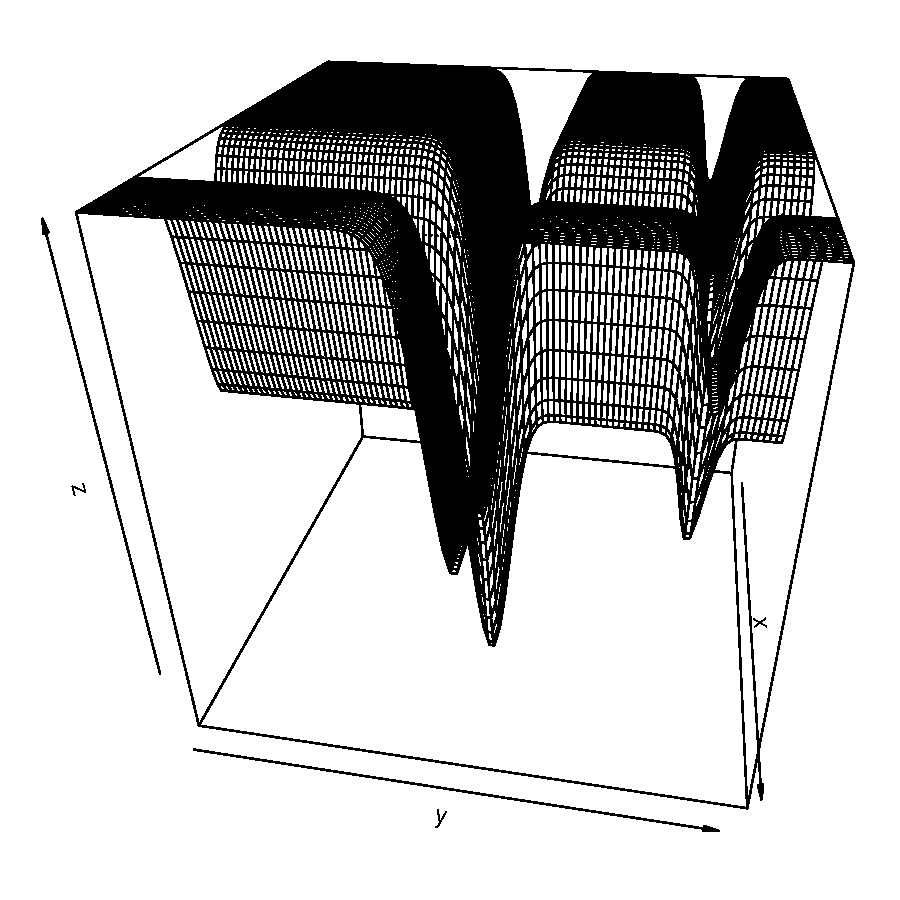
\includegraphics[width=\textwidth]{chapters/EGO/pdfs/michal_m10}
\caption{2D Michalewicz function for \(p = 10\)}
\end{subfigure}
\caption{Michalewicz function}
\end{figure}


\clearpage
\section{Numerical Experiments}\label{numerical-experiments}
This section presents the numerical results from applying Gaussian Process (GP) to the prediction functions and Efficient Global Optimization (EGO) to the minimization functions. In order to determine the effectiveness of the different initial designs, both prediction and optimization functions were taken into consideration.

We first generate different types of space-filling designs using various packages as described in Section \ref{sec:designs} and examine their performance and relationship under different criteria. For each type of design, we ran the corresponding algorithm to construct $80\times 8$ LHDs 200 times. Table \ref{tab:comparison} shows the mean and median of the various design criteria for each design type.
The design criteria are the maximin LHD criterion \eqref{eqn:maximinLHD} with $p=15$, the MaxPro criterion \eqref{eqn:MaxPro}, the centered $L_2$-discrepancy \eqref{eqn:cd}, the UPD criterion \eqref{eqn:UniPro}, and the absolute average correlation criterion \eqref{eqn:rho_ave}  defined below:
\begin{equation}\label{eqn:rho_ave}
\rho_{ave} =\frac{2}{m(m-1)}\sum_{k = 1}^m\sum_{l = k+1}^m\frac{\left|\sum_{i=1}^n\left(x_{ik}-\bar{x}_{\cdot k}\right)\left(x_{il}-\bar{x}_{\cdot l}\right)\right|}{\sqrt{\sum_{i=1}^n\left(x_{ik}-\bar{x}_{\cdot k}\right)^2 \sum_{i=1}^n\left(x_{il} -\bar{x}_{\cdot l}\right)^2}}.
\end{equation}
For all criteria, smaller values represent better designs.

As expected, each type of design performs the best under the corresponding criterion used to generate the design. For example, maximin LHD have smaller $\phi_p(D)$ values and MaxPro designs have smaller $\psi(D)$ values. In addition, random LHDs are worse than all other types of space-filling designs.
Regarding to the $\rho_{ave}$ criterion, UPDs and uniform designs (ud) are considerably better than other types of designs.
 Figure \ref{fig:comparison} gives a visualization where UPDs are fairly comparable to the uniform designs. These two types of designs have the highest correlation. From Table \ref{tab:comparison} and Figure \ref{fig:comparison}, we are capable to determine that uniform designs and UPDs are more robust than other types of designs under various design criteria. We have examined cases with different design sizes, and the conclusions are similar.

\begin{table}[!h]
\centering
\caption{\label{tab:comparison}Comparison of 100 $80\times 8$ designs using various criteria}
\centering
\begin{tabular}[t]{llrrrrr}
\toprule
\textbf{design} & \textbf{summary} & \textbf{$\phi_p(D)$} & \textbf{$\psi(D)$} & \textbf{$100CD$} & \textbf{$100\phi(D)$} & \textbf{$\rho_{ave}$}\\
\midrule
maximin & mean & 0.0231 & 90.5940 & 1.2676 & 0.0215 & 0.0289\\
\cmidrule{2-7}
 & median & 0.0231 & 83.5325 & 1.2616 & 0.0214 & 0.0289\\
\cmidrule{1-7}
MaxPro & mean & 0.0281 & 32.5730 & 1.2028 & 0.0182 & 0.0483\\
\cmidrule{2-7}
 & median & 0.0280 & 32.3859 & 1.1962 & 0.0181 & 0.0481\\
\cmidrule{1-7}
ud & mean & 0.0269 & 35.0794 & 0.7129 & 0.0088 & 0.0072\\
\cmidrule{2-7}
 & median & 0.0266 & 34.6913 & 0.7131 & 0.0088 & 0.0071\\
\cmidrule{1-7}
UniPro & mean & 0.0326 & 44.4252 & 0.9240 & 0.0084 & 0.0054\\
\cmidrule{2-7}
 & median & 0.0321 & 43.6042 & 0.9215 & 0.0084 & 0.0054\\
\cmidrule{1-7}
randomLHD & mean & 0.0402 & 125.7954 & 2.1808 & 0.0377 & 0.0883\\
\cmidrule{2-7}
 & median & 0.0385 & 116.8441 & 2.1881 & 0.0379 & 0.0891\\
\bottomrule
\end{tabular}
\end{table}

\begin{figure}%[h!tb]
\begin{adjustwidth}{-2cm}{-2cm}
\captionsetup[subfigure]{labelformat=empty}
\centering
\begin{subfigure}[b]{0.3\textwidth}
\centering
\caption{$\psi(D)\sim\phi_p(D)$}
\includegraphics[width=\textwidth]{chapters/EGO/pdfs/phi_p_psi}
\end{subfigure}
\begin{subfigure}[b]{0.3\textwidth}
\centering
\caption{$100CD \sim \phi_p(D)$}
\includegraphics[width=\textwidth]{chapters/EGO/pdfs/phi_p_cd}
\end{subfigure}
\begin{subfigure}[b]{0.3\textwidth}
\centering
\caption{$100\phi(D)\sim \phi_p(D)$}
\includegraphics[width=\textwidth]{chapters/EGO/pdfs/phi_p_eta}
\end{subfigure}
\vfill
\begin{subfigure}[b]{0.3\textwidth}
\centering
\caption{$\rho_{ave}(D)\sim \phi_p(D)$}
\includegraphics[width=\textwidth]{chapters/EGO/pdfs/phi_p_rho_ave}
\end{subfigure}
\begin{subfigure}[b]{0.3\textwidth}
\centering
\caption{$100CD \sim \psi(D)$}
\includegraphics[width=\textwidth]{chapters/EGO/pdfs/psi_cd}
\end{subfigure}
\begin{subfigure}[b]{0.3\textwidth}
\centering
\caption{$100\phi(D)\sim \psi(D)$}
\includegraphics[width=\textwidth]{chapters/EGO/pdfs/psi_eta}
\end{subfigure}
\vfill
\begin{subfigure}[b]{0.3\textwidth}
\centering
\caption{$\rho_{ave}(D)\sim \psi(D)$}
\includegraphics[width=\textwidth]{chapters/EGO/pdfs/psi_rho_ave}
%\includegraphics[scale=0.5]{chapters/EGO/pdfs/psi_rho_ave}
\end{subfigure}
\begin{subfigure}[b]{0.3\textwidth}
\centering
\caption{$100\phi(D)\sim 100CD$}
\includegraphics[width=\textwidth]{chapters/EGO/pdfs/cd_eta}
%\includegraphics[scale=0.5]{chapters/EGO/pdfs/cd_eta}
\end{subfigure}
\begin{subfigure}[b]{0.3\textwidth}
\centering
\caption{$\rho_{ave}(D)\sim 100CD$}
\includegraphics[width=\textwidth]{chapters/EGO/pdfs/cd_rho_ave}
\end{subfigure}
\begin{subfigure}[b]{0.3\textwidth}
\centering
\caption{$\rho_{ave}(D)\sim 100\phi(D)$}
\includegraphics[width=\textwidth]{chapters/EGO/pdfs/eta_rho_ave}
\end{subfigure}
\caption{Comparison of 100 $80\times 8$ LHDs using various criteria}
\label{fig:comparison}
\end{adjustwidth}
\end{figure}


\clearpage
\subsection{Prediction results}

The test functions are evaluated on various space-filling LHDs of sizes $64\times 15$ and $128\times 31$. In addition, UPDs with 8 and 16 levels are also constructed and used for model fitting and prediction with the purpose of evaluating whether the number of levels affects the performance. All designs are scaled to the function domain accordingly.
 Since the functions are of various dimensions, yet the designs used are of a pre-specified dimension, the unused dimensions are considered to be inert and serve as `noise'. This is quite common in practice whereby some inert factors are involved in an experimental study. For example, the borehole function has 8 variables, thus we have 7 inert variables when the design has 15 columns. For each design type, an ordinary kriging model with a constant trend using the mat\'ern correlation function with $\nu = 5/2$ is then fitted. To evaluate the performance of different types of designs, the normalized root mean square error is used. This is given by
% $$
% \text {Normalized RMSE}=\left[\frac{N^{-1} \sum_{i=1}^N\left\{\hat{y}\left(\x_i\right)-y\left(\x_i\right)\right\}^2}{N^{-1} \sum_{i=1}^N\left\{\bar{y}-y\left(\x_i\right)\right\}^2}\right]^{1 / 2},
% $$
$$
\text {Normalized RMSE}=\left[\frac{N^{-1} \sum_{i=1}^N\left\{\hat{y}\left(\x_i\right)-y\left(\x_i\right)\right\}^2}{N^{-1} \sum_{i=1}^N\left\{\bar{y}_{train}-y\left(\x_i\right)\right\}^2}\right]^{1 / 2},
$$
where $\x_1, \ldots, \x_N$ are the inputs of the test dataset, $y(\x_i)$ is the true response, $\hat{y}(\x_i)$ is the predicted value from the GP model, and $\bar{y}$ is the mean of the responses in the training dataset. This criterion is related to $R^2$ in regression, but it measures performance for a new test dataset and smaller values are desirable \parencite{chen2016analysis}. We used a random LHD with $N=10,000$ runs as the test dataset.

In order to reduce the randomness effect, the process is replicated 200 times. The replication  of the design generation is done via row and column permutations.  For each design type, except for the random LHD, 100 designs are generated and the best design among these 100 generated designs determined by each design type criterion is chosen as the candidate design. Using row and column permutation of the best design for each design type, 100 designs are thus generated. This method of design generation is chosen as it is almost infeasible to generate uniform designs of size $64 \times 15$ and $128\times 31$ 200 times. In particular to generate a $10\times 3$ uniform design with 10 levels using a machine equipped with a 13th Gen Intel Core\texttrademark{} i7-1360P 16-core CPU running at 2.2 GHz, it takes an average of 5.8 seconds while a machine with Intel\textregistered{} Xeon\textregistered{} Platinum 8160 CPU with 48 cores running at 2.10 GHz takes an average of 5.77 seconds. In order to use the row and column permutation, a fairly large enough design is to be used. For example to generate a $80\times 8$ UD design with 80 levels requires $\approx 439$ minutes (7.32 hours) just for one design in the first machine, while needing 432 minute (7.2 hours) in the second machine. This shows as to why permutation is the best way to do the design generation.


\begin{table}[h!tb]

\caption{\label{tab:mean_median_64x15}Means and medians of normalized RMSEs for $64\times 15$ designs}
\centering
\begin{tabular}[t]{lllllllll}
\toprule
fun &  & lhd & maximin & maxpro & ud & upd & upd16q & upd8q\\
\midrule
Borehole & mean & 0.1168 & 0.1048 & 0.1053 & \textbf{0.0936} & 0.0986 & 0.0990 & 0.1119\\
\cmidrule{2-9}
 & median & 0.1171 & 0.1044 & 0.1049 & \textbf{0.0930} & 0.0987 & 0.0986 & 0.1117\\
\cmidrule{1-9}
Circuit & mean & 0.1519 & 0.1394 & 0.1397 & \textbf{0.1286} & 0.1337 & 0.1308 & 0.1417\\
\cmidrule{2-9}
 & median & 0.1526 & 0.1383 & 0.1386 & \textbf{0.1280} & 0.1335 & 0.1298 & 0.1408\\
\cmidrule{1-9}
Currin & mean & 0.1622 & 0.1487 & 0.1480 & 0.1380 & 0.1333 & \textbf{0.1273} & 0.1326\\
\cmidrule{2-9}
 & median & 0.1606 & 0.1473 & 0.1479 & 0.1372 & 0.1330 & \textbf{0.1273} & 0.1328\\
\cmidrule{1-9}
Gfunction & mean & 0.8092 & 0.8618 & 0.8328 & 0.8540 & 0.7795 & 0.7830 & \textbf{0.7423}\\
\cmidrule{2-9}
 & median & 0.7996 & 0.8704 & 0.8237 & 0.8757 & 0.7642 & 0.7598 & \textbf{0.7167}\\
\cmidrule{1-9}
OakleyOhagan & mean & 0.2461 & 0.2358 & 0.2329 & 0.2284 & 0.2277 & \textbf{0.2258} & 0.2300\\
\cmidrule{2-9}
 & median & 0.2460 & 0.2364 & 0.2324 & 0.2278 & 0.2276 & \textbf{0.2257} & 0.2279\\
\cmidrule{1-9}
Piston & mean & 0.2351 & 0.2127 & 0.2195 & \textbf{0.2101} & 0.2137 & 0.2146 & 0.2254\\
\cmidrule{2-9}
 & median & 0.2317 & 0.2103 & 0.2172 & \textbf{0.2065} & 0.2113 & 0.2149 & 0.2227\\
\cmidrule{1-9}
Rosenbrock & mean & 0.4134 & 0.4051 & 0.3943 & 0.3708 & 0.3672 & \textbf{0.3583} & 0.3655\\
\cmidrule{2-9}
 & median & 0.4115 & 0.4053 & 0.3908 & 0.3699 & 0.3669 & \textbf{0.3580} & 0.3659\\
\cmidrule{1-9}
Wingweight & mean & 0.1520 & 0.1275 & 0.1367 & \textbf{0.1244} & 0.1337 & 0.1310 & 0.1355\\
\cmidrule{2-9}
 & median & 0.1496 & 0.1268 & 0.1352 & \textbf{0.1239} & 0.1334 & 0.1309 & 0.1352\\
\bottomrule
\end{tabular}
\end{table}

\begin{figure}%[h!tb]
\begin{adjustwidth}{-2cm}{-2cm}
\captionsetup[subfigure]{labelformat=empty}
\centering
\begin{subfigure}[b]{0.35\textwidth}
\centering
\caption{Borehole}
\includegraphics[width=\textwidth]{chapters/EGO/pdfs/Borehole_64x15}
\end{subfigure}
\begin{subfigure}[b]{0.35\textwidth}
\centering
\caption{Circuit}
\includegraphics[width=\textwidth]{chapters/EGO/pdfs/Circuit_64x15}
\end{subfigure}
\begin{subfigure}[b]{0.35\textwidth}
\centering
\caption{Currin}
\includegraphics[width=\textwidth]{chapters/EGO/pdfs/Currin_64x15}
\end{subfigure}
\vfill
\begin{subfigure}[b]{0.35\textwidth}
\centering
\caption{Gfunction}
\includegraphics[width=\textwidth]{chapters/EGO/pdfs/Gfunction_64x15}
\end{subfigure}
\begin{subfigure}[b]{0.35\textwidth}
\centering
\caption{OakleyOhagan}
\includegraphics[width=\textwidth]{chapters/EGO/pdfs/OakleyOhagan_64x15}
\end{subfigure}
\begin{subfigure}[b]{0.35\textwidth}
\centering
\caption{Piston}
\includegraphics[width=\textwidth]{chapters/EGO/pdfs/Piston_64x15}
\end{subfigure}
\vfill
\begin{subfigure}[b]{0.35\textwidth}
\centering
\caption{4D Rosenbrock}
\includegraphics[width=\textwidth]{chapters/EGO/pdfs/Rosenbrock4d_64x15}
\end{subfigure}
\begin{subfigure}[b]{0.35\textwidth}
\centering
\caption{Wingweight}
\includegraphics[width=\textwidth]{chapters/EGO/pdfs/Wingweight_64x15}
\end{subfigure}
\caption{Normalized RMSEs for various test functions and $64\times 15$ designs}
\label{fig:boxplots_64x15}
\end{adjustwidth}
\end{figure}

Figure \ref{fig:boxplots_64x15} shows the normalized RMSEs for the various test functions using various $64\times15$ designs. The mean and median RMSEs are also obtained and are reported in Table \ref{tab:mean_median_64x15}.
A general conclusion is that the use of uniform designs and uniform projection designs in prediction is efficient as they result in minimal normalized RMSEs for most of the test functions, compared to the other types of designs. This could be attributed to their robustness in nature. On the other hand, the random LHD is often the worst as expected with one exception. For the 9-dimensional G-function, the maximin, MaxPro and uniform LHDs perform worse than the random LHD whereas all three of the UPDs perform better than the random LHD. In particular the 8-level UPD  (upd8q) performs the best in this case.

Among all space-filling designs, the UPD appears to be the most robust as it is never worse than the random LHD. Also it is better than the maximin and  MaxPro designs with one exception for the Wingweight function, where the maximin design is better. In addition, the 16-level UPD (upd16q) performs better than the 8-level UPD except for the case of the G-function. At the same time 16-level UPD performs better than the 64-level UPD. This gives the notion of the importance of the number of levels. A fair enough number of levels in comparison to the number of runs is important in prediction. While in physical experiments, 3-5 levels are enough, in computer experiments, more levels are needed.

The conclusions reached are further cemented by observing the results obtained when using $128\times 31$ design size for training and predicting on the test dataset with 10,000 runs. Here 8-level UPD is not used as it produces many outliers which would distort the visual comparison of the results. The 16-level UPD still has the best performance in most of the test functions; see Table \ref{tab:mean_median_128x31} and Figure \ref{fig:boxplots_128x31}.


\begin{table}[h!tb]

\caption{\label{tab:mean_median_128x31}Means and medians of normalized RMSEs for $128\times 31$ designs}
\centering
\begin{tabular}[t]{llllllll}
\toprule
fun &  & lhd & maximin & maxpro & ud & upd & upd16q\\
\midrule
Borehole & mean & 0.1624 & 0.1451 & 0.1511 & \textbf{0.1366} & 0.1425 & 0.1408\\
\cmidrule{2-8}
 & median & 0.1625 & 0.1449 & 0.1508 & \textbf{0.1365} & 0.1426 & 0.1406\\
\cmidrule{1-8}
Circuit & mean & 0.1920 & 0.1742 & 0.1798 & 0.1676 & 0.1709 & \textbf{0.1630}\\
\cmidrule{2-8}
 & median & 0.1908 & 0.1739 & 0.1784 & 0.1672 & 0.1704 & \textbf{0.1631}\\
\cmidrule{1-8}
Currin & mean & 0.1960 & 0.1818 & 0.1815 & \textbf{0.1730} & 0.1747 & 0.4376\\
\cmidrule{2-8}
 & median & 0.1949 & 0.1809 & 0.1799 & 0.1724 & 0.1744 & \textbf{0.1582}\\
\cmidrule{1-8}
Gfunction & mean & 0.7697 & 0.8550 & 0.8074 & 0.8682 & 0.7724 & \textbf{0.7297}\\
\cmidrule{2-8}
 & median & 0.7642 & 0.8336 & 0.7894 & 0.8677 & 0.7599 & \textbf{0.7119}\\
\cmidrule{1-8}
OakleyOhagan & mean & 0.3166 & 0.2769 & 0.3006 & \textbf{0.2752} & 0.2865 & 0.2797\\
\cmidrule{2-8}
 & median & 0.3156 & 0.2763 & 0.2988 & \textbf{0.2748} & 0.2854 & 0.2794\\
\cmidrule{1-8}
Piston & mean & 0.2699 & 0.2504 & 0.2601 & \textbf{0.2475} & 0.2535 & 0.2483\\
\cmidrule{2-8}
 & median & 0.2703 & 0.2510 & 0.2593 & \textbf{0.2475} & 0.2525 & 0.2478\\
\cmidrule{1-8}
Rosenbrock & mean & 0.4257 & 0.4204 & 0.4105 & 0.3916 & 0.3975 & \textbf{0.3724}\\
\cmidrule{2-8}
 & median & 0.4248 & 0.4189 & 0.4102 & 0.3909 & 0.3977 & \textbf{0.3720}\\
\cmidrule{1-8}
Wingweight & mean & 0.2037 & \textbf{0.1748} & 0.1900 & 0.1756 & 0.1821 & 0.3112\\
\cmidrule{2-8}
 & median & 0.2027 & 0.1745 & 0.1879 & 0.1752 & 0.1819 & \textbf{0.1669}\\
\bottomrule
\end{tabular}
\end{table}

\begin{figure}%[h!tb]
\begin{adjustwidth}{-2cm}{-2cm}
\captionsetup[subfigure]{labelformat=empty}
\centering
\begin{subfigure}[b]{0.35\textwidth}
\centering
\caption{Borehole}
\includegraphics[width=\textwidth]{chapters/EGO/pdfs/Borehole_128x31}
\end{subfigure}
\begin{subfigure}[b]{0.35\textwidth}
\centering
\caption{Circuit}
\includegraphics[width=\textwidth]{chapters/EGO/pdfs/Circuit_128x31}
\end{subfigure}
\begin{subfigure}[b]{0.35\textwidth}
\centering
\caption{Currin}
\includegraphics[width=\textwidth]{chapters/EGO/pdfs/Currin_128x31}
\end{subfigure}
\vfill
\begin{subfigure}[b]{0.35\textwidth}
\centering
\caption{Gfunction}
\includegraphics[width=\textwidth]{chapters/EGO/pdfs/Gfunction_128x31}
\end{subfigure}
\begin{subfigure}[b]{0.35\textwidth}
\centering
\caption{OakleyOhagan}
\includegraphics[width=\textwidth]{chapters/EGO/pdfs/OakleyOhagan_128x31}
\end{subfigure}
\begin{subfigure}[b]{0.35\textwidth}
\centering
\caption{Piston}
\includegraphics[width=\textwidth]{chapters/EGO/pdfs/Piston_128x31}
\end{subfigure}
\vfill
\begin{subfigure}[b]{0.35\textwidth}
\centering
\caption{4D Rosenbrock}
\includegraphics[width=\textwidth]{chapters/EGO/pdfs/Rosenbrock4d_128x31}
\end{subfigure}
\begin{subfigure}[b]{0.35\textwidth}
\centering
\caption{Wingweight}
\includegraphics[width=\textwidth]{chapters/EGO/pdfs/Wingweight_128x31}
\end{subfigure}
\caption{Normalized RMSEs for various test functions and $128 \times 31$ designs}
\label{fig:boxplots_128x31}
\end{adjustwidth}
\end{figure}

From Figure \ref{fig:boxplots_128x31} we see that the Currin and the wing weight functions  produce a few large RMSE values, likely due to the failure of the optimization routine when fitting the kriging model. These outliers distort the display of the boxplots even though the other RMSE values are generally concentrated below the RMSE value of the other functions. For a fair comparison, we got rid of these outliers and plotted the rest as shown in Figure \ref{fig:no_outlier}.

\begin{figure}%[h!tb]
\captionsetup[subfigure]{labelformat=empty}
\centering
\begin{subfigure}[b]{0.45\textwidth}
\centering
\caption{Currin}
\includegraphics[width=\textwidth]{chapters/EGO/pdfs/Currin_128x31_no_outlier}
\end{subfigure}
\begin{subfigure}[b]{0.45\textwidth}
\centering
\caption{Wing Weight}
\includegraphics[width=\textwidth]{chapters/EGO/pdfs/Wingweight_128x31_no_outlier}
\end{subfigure}
\caption{Normalized RMSEs for Currin and Wing Weight functions without the outliers}
\label{fig:no_outlier}
\end{figure}


\clearpage
\subsection{Minimization results}

We consider four types of space-filling designs for sequential minimization: random LHDs, maximin LHDs, MaxPro LHDs and UPDs. The test functions are evaluated at $n_0 = 10\times m$ initial points, apart from the Branin function which is evaluated at $n_0 = 10$ initial points. These functions are then minimized using the EGO approach. We use the function fastEGO.nsteps in the R DiceOptim package to sequentially add a point at a time with $n_1$ steps. For each step, the cumulative minimum is recorded. This process is replicated 200 times.






\begin{figure}%[h]
\captionsetup[subfigure]{labelformat=empty}
\centering
\begin{subfigure}[b]{0.3\textwidth}
\centering
\caption{Branin}
\includegraphics[width=\textwidth]{chapters/EGO/pdfs/branin_lineplot}
\end{subfigure}
%
\begin{subfigure}[b]{0.3\textwidth}
\centering
\caption{Camel Six}
\includegraphics[width=\textwidth]{chapters/EGO/pdfs/camel6_lineplot}
\end{subfigure}
%\centering
\begin{subfigure}[b]{0.3\textwidth}
\centering
\caption{Goldstein-Price}
\includegraphics[width=\textwidth]{chapters/EGO/pdfs/goldpr_lineplot}
\end{subfigure}
\caption*{\includegraphics [scale=0.3,trim={2cm 7.3cm 0 7cm},clip]{chapters/EGO/pdfs/legend}}
\caption{Minimization path for 2 dimensional test functions}
\label{fig:2dimension}
\end{figure}

Figure \ref{fig:2dimension} shows the average minimal values at each step, together with the 2 standard error bar, of the resulting minimization path with $n_1=20$ added points for three 2-dimensional test functions.
For the Branin function,  MaxPro designs and UPDs yield smaller y-values at early stages than maximin and random LHDs. The difference gradually diminishes over the sequential optimization process. After 15 additional points, all the methods have the same y-value indicating that the function minimum has been achieved. The result is similar for the Camel Six function. For the Goldstein-Price function, the UPD maintains its advantage over others even after 20 steps.




% 6D



% 8D











\begin{figure}%[h!]
\captionsetup[subfigure]{labelformat=empty}
\centering
\begin{subfigure}[b]{0.3\textwidth}
\centering
\caption{4D Ackley}
\includegraphics[width=\textwidth]{chapters/EGO/pdfs/ackley4_lineplot}
\end{subfigure}
\begin{subfigure}[b]{0.3\textwidth}
\centering
\caption{4D Levy}
\includegraphics[width=\textwidth]{chapters/EGO/pdfs/levy4_lineplot}
\end{subfigure}
\begin{subfigure}[b]{0.3\textwidth}
\centering
\caption{4D Michalewicz}
\includegraphics[width=\textwidth]{chapters/EGO/pdfs/michal_lineplot}
\end{subfigure}
\begin{subfigure}[b]{0.3\textwidth}
\centering
\caption{6D Ackley}
\includegraphics[width=\textwidth]{chapters/EGO/pdfs/ackley6_lineplot}
\end{subfigure}
\begin{subfigure}[b]{0.3\textwidth}
\centering
\caption{6D Levy}
\includegraphics[width=\textwidth]{chapters/EGO/pdfs/levy6_lineplot}
\end{subfigure}
\begin{subfigure}[b]{0.3\textwidth}
\centering
\caption{6D Michalewicz}
\includegraphics[width=\textwidth]{chapters/EGO/pdfs/michal6_lineplot}
\end{subfigure}
\begin{subfigure}[b]{0.3\textwidth}
\centering
\caption{8D Ackley}
\includegraphics[width=\textwidth]{chapters/EGO/pdfs/ackley8_lineplot}
\end{subfigure}
\begin{subfigure}[b]{0.3\textwidth}
\centering
\caption{8D Levy}
\includegraphics[width=\textwidth]{chapters/EGO/pdfs/levy8_lineplot}
\end{subfigure}
\begin{subfigure}[b]{0.3\textwidth}
\centering
\caption{8D Michalewicz}
\includegraphics[width=\textwidth]{chapters/EGO/pdfs/michal8_lineplot}
\end{subfigure}
\begin{subfigure}[b]{0.3\textwidth}
\centering
%\caption{8D rosenbrock}
\end{subfigure}
\caption*{\includegraphics [scale=0.3,trim={2cm 7.3cm 0 7cm},clip]{chapters/EGO/pdfs/legend}}
\caption{Minimization path for test functions with varying dimensions}
\label{fig:lineplots}
%\end{adjustwidth}
\end{figure}


The results presented above are not unique. They are determined by the computation of the first y-value from the initial design. The design that initially produces the least function value tends to generally converge faster to the function minimum, as the sequential points majorly depend on the expected improvement with influence from the design type. This indicates that the choice of the initial design for optimization is quite significant. A poor initial design will yield poor objective values at the initialization stage which will lead to slower convergence.

As the number of iterations (nsteps) increases, the influence of the initial design type on the optimization process diminishes. Initially, the choice of design strategy can play a significant role in guiding the search for the global optimum. However, as more sample points are iteratively added based on the acquisition function, the optimization process becomes increasingly driven by the updated GP model. This model incorporates all collected data points, thereby reducing the relative impact of the initial design. Consequently, the optimization converges towards the global optimum, and differences attributed to the initial design strategy become less pronounced.

Though this is the case, in high dimensional setup, or using complicated functions, the number of sequentially added points needed for convergence might be quite large. With a limited budget, the effect of initial design could be profound.

Figure \ref{fig:lineplots} shows the minimization path for 3 other test functions with varying dimensions from 4 to 8.
One striking observation is the decreasing efficiency of using maximin designs when the dimension increases. At lower dimensions,  maximin designs fairly compete with the other designs but as the dimensions increase to 6 and 8, it is observed that the maximin designs do poorly. This is even after increasing the number of steps to 30 or more. We also note that  MaxPro designs are worse than random LHDs and UPDs for the Ackley and Levy function. Overall, UPDs are robust and perform well under all situations, especially in high dimensions and complicated test functions.

\section{Concluding Remarks}
In conclusion, the numerical evaluation of Gaussian Process (GP) and Efficient Global Optimization (EGO) techniques reveal that the uniform design (UD) and uniform projection design (UPD)  stand out for their robustness and efficiency. When compared across various design criteria, the UD and UPD consistently demonstrate superior performance. The extensive experimentation, including the generation of 100 designs and their permutations, highlighting the efficiency of the uniform designs in reducing normalized root mean square error in prediction tasks.
Notably, the UPD with 16 levels proved to be particularly effective, underscoring the importance of having a sufficiently large number of levels in design, yet it is not necessary to use LHDs with the number of levels being equal to the number of runs when the latter is large.

The comparative analysis of different initial designs for EGO further confirmed the efficacy of UPDs. As evidenced by the results, UPDs converged more quickly to the function minimum compared to other design methods. Although the differences in optimization outcomes among design strategies became less pronounced with more iterations, the initial design choice had a significant impact at early stages, which could prolong to later stages when we encounter complicated optimization tasks in high dimensions. This observation underscores the value of selecting a good design strategy for enhancing the efficiency of the optimization process. In conclusion, UPDs are simple to construct, offering a  feasible solution for large-scale, high-dimensional prediction and optimization tasks.


However, the results also revealed some limitations, particularly with distance-based designs like the maximin criterion in high-dimensional spaces. One reason as to why this might be the case is because of the use of Euclidean distance as the criterion to be optimized by the maximin design yet it is well documented that Euclidean distance is not a good metric in high dimensions. In high dimensions, the natural intuition which comes from our three-dimensional world fails and thus do not apply \parencite{domingos2012few}. Taking an example of Gaussian distribution, in high dimensions, most of the mass of a multivariate Gaussian distribution is not near the mean, but in an increasingly distant ``shell" around it; and most of the volume of a high dimensional orange is in the skin, and not the pulp. If a constant number of points is distributed uniformly in a high-dimensional hypercube, beyond some dimensionality most points are closer to a face of the hypercube than to their nearest neighbor. When a hypersphere is approximated by inscribing it in a hypercube, in high dimensions almost all the volume of the hypercube is outside the hypersphere \parencite{domingos2012few}. At the same time, in high dimensions, the ratio between the nearest and farthest points using Euclidean distance metric approaches 1, i.e., the points essentially become uniformly distant from each other \parencite{aggarwal2001surprising}. Thus, as all points are essentially uniformly distant from each other, the distinction is meaningless. This indicates as to why the Euclidean distance would therefore not be a good measure of distance in high dimensions. Since the spreading of points using the maximin design is done using the Euclidean distance,% these points will mostly cover the empty space rather than the surface where the function is defined, hence making it be inefficient as compared to the other methods.
the design will experience the issues highlighted above making it  inefficient as compared to the other methods. Perhaps this phenomenon also impacts the MaxPro designs, making the efficiency of the MaxPro design to decline as the dimensions increases as seen in Figure \ref{fig:lineplots}. Though this is not known.

As the UPD focusing on 2-dimensional uniformity, it is not highly impacted by the curse of dimensionality. Thereby retaining its high performance in comparison to the distance based designs with regards to minimizing high dimensional functions. The inefficacy of the maximin design in higher dimensions, due to the limitations of Euclidean distance metrics, suggests that such distance-based methods may not be well-suited for complex high-dimensional problems. Conversely, the UPD's use of the centered $L_2$-discrepancy criterion allows it to mitigate the curse of dimensionality, maintaining its effectiveness across various dimensions. This highlights the need for careful consideration of design criteria and metrics in high-dimensional optimization tasks to ensure accurate and efficient results.

%\printbibliography




%\end{document}
%\documentclass[12pt,a4paper, notitlepage]{article}
%\usepackage[utf8]{inputenc}
%\usepackage{sectsty}
%\usepackage[graphicx]{realboxes}
%\usepackage{graphicx}
%\usepackage{subcaption}
%\usepackage{multirow}
%\usepackage{multicol}
%\usepackage{graphicx}
%\usepackage[margin=2.5cm ]{geometry}
%\usepackage{algpseudocode}
%\usepackage{algorithm}
%\usepackage{amsmath, amsfonts}
%\usepackage{float}
%\usepackage{booktabs}
%\usepackage{makecell}
%\usepackage[hidelinks,citecolor=blue, colorlinks]{hyperref}
%\usepackage[style=authoryear, sorting=nyt, backend=bibtex,sortcites=true]{biblatex}
%\addbibresource{../../include/reference.bib}
%
%\hypersetup{colorlinks,linkcolor={blue},citecolor={blue},urlcolor={red}}
%
%\sectionfont{\fontsize{13}{15}\selectfont}
%\subsectionfont{\fontsize{10}{10}\selectfont}
%%\addbibresource{reference.bib}
%
\chapter{Kriging Based Sequential Region Shrinkage with EGO for  Hyperparameter Optimization }
%\author{Onyambu, S.  }
%%\date{}
%
%\providecommand{\keywords}[1]
%{
%  \Large
%  \textbf{\textit{Keywords---}} #1
%}
%
%\usepackage{fullpage}
%\renewcommand{\baselinestretch}{1.25}% {1.25}
%\renewcommand{\arraystretch}{1.1}
%\renewcommand{\tabcolsep}{4pt}
%
%%% trace revision using color
%%% trace revision using color
%\newcommand{\reva}[1]{{\color{red} #1}}
%\newcommand{\revb}[1]{{\color{blue} #1}}
%\newcommand{\revc}[1]{{\color{cyan} #1}}
%\newcommand{\revd}[1]{{\color{blue} #1}}
%\newcommand{\reve}[1]{{\color{blue} #1}}
%%% to remove color, uncomment the following
%%\renewcommand{\reva}[1]{{#1}}  % remove color
%%\renewcommand{\revb}[1]{{#1}}
%%\renewcommand{\revc}[1]{{#1}}  % remove color
%%\renewcommand{\revd}[1]{{#1}}
%%\renewcommand{\reve}[1]{{#1}}
%
%\usepackage{amsmath,amssymb}
%\newcommand{\X}{\boldsymbol{X}}
%\newcommand{\Y}{\boldsymbol{Y}}
%\newcommand{\x}{\boldsymbol{x}}
%%\renewcommand{\u}{\boldsymbol{u}}
%\newcommand{\y}{\boldsymbol{y}}
%\newcommand{\z}{\boldsymbol{z}}
%\newcommand{\w}{\boldsymbol{w}}
%\newcommand{\R}{\boldsymbol{R}}
%\newcommand{\Rinv}{\boldsymbol{R}^{-1}}
%\newcommand{\one}{\mathbf{1}}
%\newcommand{\cov}{\textrm{Cov}}
%
%\usepackage{Sweave}
%
%
%
%\begin{document}
%
%
%\maketitle
%\begin{abstract}
%   We propose a Kriging based sequential region shrinking method, which invokes  efficient global optimization (EGO) algorithm while sequentially determining a reduced region of interest based on a proportion of most promising data points. The efficiency of the proposed method is demonstrated on various  well known physical test functions. We also  compare the method to well known hyper-parameter tuning methods. Experimental results on datasets indicates that the method uses fewer resources and has an edge to the commonly used hyper-parameter tuning methods like grid and random search and also to other Bayesian optimization such as TREGO.
%\end{abstract}
%
%
\section{Introduction}



Black-box optimization is a key challenge in many fields, including engineering, finance, and machine learning. It involves finding the optimal solution to a complex function that is either expensive or impossible to evaluate analytically. Formally, this can be expressed as:
$$
\x^* = \underset{\x \in \Omega}{\arg \min} f(\x),
$$
where \(\Omega\) represents the search space of \(\x\). Optimizing \(f(\x)\) is a non-trivial task, typically requiring either derivative-based or derivative-free methods. Derivative-based methods depend on the calculation of the objective function's derivatives, making them suitable when \(f(\x)\) is smooth and differentiable, and its derivatives are easy to compute. However, in many real-world scenarios, the function is unknown or difficult to differentiate, making derivative-free methods preferable. These methods are especially useful in cases of black-box functions, that is, where the objective is not directly accessible.

Hyper-parameter Optimization (HPO) is a classic example of a black-box optimization problem, where the goal is to select the best set of hyper-parameters for a learning algorithm. These hyper-parameters are typically set before training and they control various aspects of the model. They include the learning rate, regularization, and the choice of the optimization algorithm. The model's performance can vary significantly based on the hyper-parameters chosen \parencite{feurer2019hyperparameter}, with results sometimes fluctuating drastically depending on the architecture \parencite{liu2018darts}. Several methods are widely used for HPO, including grid search, random search \parencite{bergstra2012random}, and Bayesian optimization \parencite{pelikan1999boa}.

Grid search systematically evaluates the model's performance for every combination of hyper-parameters within a predefined grid, choosing the configuration that yields the best result. Random search, on the other hand, samples hyper-parameters randomly from a predefined distribution and selects the best-performing configuration. Bayesian optimization constructs a probabilistic model of the objective function by combining prior knowledge with previously evaluated configurations. The posterior model is then optimized using an acquisition function, and the process is repeated until no further improvements can be made \parencite{brochu2010tutorial}.

While grid search and random search are simple and easy to implement, they become computationally expensive, especially in high-dimensional hyper-parameter spaces. Bayesian optimization is typically more efficient and effective for HPO \parencite{snoek2012practical}. One way to enhance the efficiency of Bayesian optimization is through the use of a surrogate model, which approximates the objective function and directs the search toward promising regions of the hyper-parameter space \parencite{jones1998efficient}.

Bayesian optimization has gained popularity in solving black-box optimization problems due to its ability to handle noisy and non-convex functions, which are common in real-world scenarios. The probabilistic surrogate model used in Bayesian optimization is typically a Gaussian Process (GP), which is a flexible and a powerful tool for modeling complex functions \parencite{rasmussen2006gaussian}. GPs can predict the value of the objective function at unexplored points while also providing an estimate of the uncertainty of these predictions.

In this paper, we propose a Kriging-based region shrinkage method that builds on Efficient Global Optimization (EGO) \parencite{jones1998efficient}. The method sequentially refines the region of interest (ROI) based on a proportion of most informative data points, progressively shrinking the search space by reducing the size of the interval for each hyper-parameter at each step. This approach allows us to focus more precisely on promising regions. By using EGO, the method balances exploration and exploitation within the domain.

The effectiveness of the proposed method is demonstrated using several well-known physical test functions from the Virtual Library of Simulation Experiments \parencite{simulationlib}. We compare our approach to existing optimization methods and show that the proposed derivative-free method achieves results on par with or exceeding expectations. Empirical results on DE hyperparameter optimization for constructing uniform projection designs show that our method requires fewer computational resources while performing comparably to, or better than, traditional hyper-parameter tuning methods such as grid search and random search. Although the theoretical guarantees are limited, the empirical results indicate strong potential for practical applications.

\section{Background Theories}
\subsection{Related Work}
In pursuit of minimizing loss, numerous optimization techniques based on the Bayesian approach have been developed. While some methods emphasize dimensionality reduction to enhance computational efficiency, the majority focus on reducing the size of the search space, commonly referred to as variable interval size reduction. The work presented here falls within this category.

Among the various strategies explored are the Controlled Gutmann-RBF (CG-RBF) method \parencite{regis2007improved}, the Trust Region Implementation in Kriging-based optimization with Expected Improvement (TRIKE) \parencite{regis2016trust}, and the Trust-Region framework for Efficient Global Optimization (TREGO) \parencite{diouane2023trego}. Although many of these methods confine the search to a local region, the TREGO method alternates between local and global searches, returning to the global scale search after a successful local search.

In TREGO, a local search is conducted when an iteration fails to achieve meaningful progress, meaning there is no significant improvement over the current best solution. Repeated failures progressively reduce the size of the local search space, while successful iterations trigger a global search. However, this process can lead to slow convergence.

To address this, we propose a modification: successful iterations will continue to focus on a reduced local search space, while unsuccessful iterations will initiate a global search. Here, a successful iteration is defined as one in which a point is found with a lower function value than any previously evaluated. We show that this proposed method leads to faster convergence compared to existing techniques, particularly TREGO.

\iffalse %
\subsection{Kriging}

Kriging, first introduced by South African geostatistician Danie Krige \parencite{krige1951statistical}, is a widely used method for interpolating intermediate values. These values are modeled using a Gaussian Process (GP), governed by prior covariances. Kriging provides both a probabilistic prediction of the output variable and an estimate of the prediction's uncertainty \parencite{chevalier2014kriginv}. It is often more reliable than other interpolation methods, such as smoothing splines. The interpolated values produced by Kriging are considered the best linear unbiased predictors, assuming the predictors are noise-free \parencite{roustant2012dicekriging}.

Kriging assumes that the output \(\y\) is the sum of a known deterministic trend function \(\mu: \x \in D \rightarrow \mu(\x) \in \mathbb{R}\) and a centered, square-integrable process \(Z\):

\begin{equation}
    Y(x) = \mu(x) + Z(x)
\end{equation}

Here, \(\mu(x)\) represents the trend, and \(Z(x)\) is a stationary GP with zero mean and a known covariance function \(\psi\).

In Universal Kriging (UK), the trend \(\mu(\x)\) is known up to a set of linear trend coefficients. This trend is modeled as a linear combination of fixed basis functions \(f_i\):

\[
\mu(\x) = \sum_{i=1}^k \beta_i f_i(\x)
\]

UK involves deriving the best linear predictors of \(\y\) based on observed data \(\y(\x)\), while estimating the coefficient vector \(\beta = (\beta_1, \dots, \beta_p)^\top\) dynamically. If the basis functions reduce to a constant, UK becomes ordinary Kriging (OK) \parencite{roustant2012dicekriging}.

The covariance function \(\psi\) fully characterizes the behavior of the Gaussian Process \(Z(\x)\), defined as:

\begin{equation}
\psi(x_i, x_j) = \operatorname{Cov} \left( Z(x_i), Z(x_j) \right) = \sigma^2 \prod_{l=1}^{d} K(h_l ; \theta_l)
\end{equation}

Here, \(\sigma^2\) is the process variance, \(h_l = |x_{i,l} - x_{j,l}|\) is the difference between the \(l\)-th components of \(x_i\) and \(x_j\), and \(d\) is the dimension of \(\x\). For stationary GPs, the mean and covariance remain constant over time. The correlation function \(K(h_l ; \theta_l)\) depends on the parameter \(\theta_l\), which must be positive for the correlation function to be valid. These parameters, often referred to as characteristic length-scales, are typically chosen to be interpretable in the same units as the corresponding variables \parencite{rasmussen2006gaussian}.

Popular choices for correlation functions include the Gaussian, Mat\'ern, and power-exponential families. The Mat\'ern function with \(\nu = 5/2\) is often preferred. It is defined as:

\[
K(h; \theta) = \left( 1 + \frac{\sqrt{5} h}{\theta} + \frac{5 h^2}{3 \theta^2} \right) \exp \left( -\frac{\sqrt{5} h}{\theta} \right)
\]

The Gaussian correlation function, \(K(h; \theta) = \exp \left( -\frac{h^2}{2\theta^2} \right)\), results in sample paths of \(Z(\x)\) that are too smooth, having derivatives of all orders. This can lead to numerical problems, such as nearly singular covariance matrices during model estimation \parencite{martin2005use}. In contrast, the Mat\'ern function with \(\nu = 3/2\) produces rougher paths, while the \(\nu = 5/2\) variant offers a good balance of smoothness. For this reason, the Mat\'ern function with \(\nu = 5/2\) is commonly recommended in practice \parencite{martin2005use}. Figure \ref{fig:matern} illustrates the relationship between \(h\) and \(K(h; \theta)\) for the Mat\'ern function.

\begin{figure}
    \centering
    \includegraphics{chapters/RSO/pdfs/matern correlation.png}
    \caption{Caption}
    \label{fig:matern}
\end{figure}


\subsection{The Expected Improvement (EI)}
The expected improvement (EI) is a measure of how promising a particular set of inputs is in terms of improving the objective function value. Evaluating the objective function at multiple points is often costly, particularly when derivative information is unavailable, and gradient-based methods cannot be applied. Similarly, meta-heuristic methods, such as genetic algorithms, are often impractical due to limited evaluation budgets \parencite{roustant2012dicekriging}. To address these limitations, \textcite{jones1998efficient} introduced the use of the Kriging model as a surrogate to estimate the expected improvement of new inputs over the current best solution. When minimizing, the key idea is that a newly sampled point, \( X_{n+1} \), will yield an improvement of \(\min(y_1, \dots, y_n) - y_{n+1}\) if the new function evaluation \(y_{n+1}\) is smaller than the current best evaluation. Otherwise, the improvement is zero. Here, \(n\) is the number of observations in the design matrix \(\x\).

The expected improvement at a point \(\x\) is computed as:

\[
EI(x) = \mathbb{E}\left[\max(y_{min} - y(x), 0)\right]
\]

where \(y_{min} = \min(y_1, \dots, y_n)\) and \(y(x)\) is the predicted value of the objective function at \(\x\), assumed to follow a normal distribution \(y(x) \sim \mathcal{N}(\hat{y}, s^2)\), with \(\hat{y}\) being the predicted value and \(s\) the standard error given by the Kriging model.

Since the actual improvement is unknown before sampling, it must be estimated. Through integration by parts, the expected improvement can be derived in closed form \parencite{jones1998efficient}:

\[
\mathrm{EI}(\x) = (\min (\y)-\mu(\x)) \Phi\left(\frac{\min (\y)-\mu(\x)}{\sigma(\x)}\right)+\sigma(\x) \phi\left(\frac{\min (\y)-\mu(\x)}{\sigma(\x)}\right)
\]

where \(\Phi\) and \(\phi\) are the cumulative distribution and probability density functions of the standard normal distribution, respectively. This criterion is particularly useful for sequential optimization, as it is zero at already-sampled points and non-negative elsewhere. It favors exploration of regions with high uncertainty (large predicted variances) while also exploiting regions with promising function evaluations (high predicted means) \parencite{jones1998efficient}.

The smoothness of the EI function-derived from the smooth predictive mean \(\mu(x)\) and variance \(\sigma(x)\) of the Gaussian process, as well as the smoothness of \(\Phi\) and \(\phi\)-enables the use of gradient-based methods. This allows efficient optimization of EI using algorithms like BFGS (Broyden-Fletcher-Goldfarb-Shanno), which is commonly used to find the point that maximizes the expected improvement.
\fi%

\subsection{The Efficient Global Optimization (EGO) Algorithm}

The Efficient Global Optimization (EGO) algorithm builds upon the Expected Improvement (EI) criterion to sequentially explore the objective function. It begins with an initial design (typically a Latin hypercube) and iteratively visits the global maximizer of the EI criterion. At each step, the Kriging surrogate model is updated, including the re-estimation of hyperparameters, based on newly sampled points. This process continues until a convergence criterion is met or the budget of function evaluations is exhausted \parencite{roustant2012dicekriging}. Algorithm \ref{alg:ego2} summarizes the procedure.

\begin{algorithm}%[H]
    \caption{EGO algorithm}\label{alg:ego2}
    \begin{algorithmic}[1]
        \Require $\X$, $f$ = function to be minimized, $n_{new}$=number of points to add
        \State Evaluate $f$ at the design points $\X$; $\y=f(\X)$
        \State Build a kriging model based on $\X$ and $\y$

    \For{$i$ in $1$ to $n_{new}$}
        \State Find $\x^* \gets \arg\max_{\x}\mathrm{E}[I(\x)]$
        \State Evaluate $y^* \gets f(\x^*)$
        \State Update $\X$ and $\y$ with the new point $\x^*$ and response $y^*$
        \State Update the kriging model
\EndFor
\State Return $\X, \y$
\end{algorithmic}
\end{algorithm}


The EGO algorithm has proven to be highly effective and is frequently used in optimization problems where the number of objective function evaluations is severely limited. It is considered as one of the reference methods for global optimization in moderate-dimensional problems (typically \(d \leq 10\)) \parencite{jones2001taxonomy}.

\subsection{The Trust Region EGO (TREGO)}
Proposed by \textcite{diouane2023trego}, Trust Region Efficient Global Optimization (TREGO) operates by searching within a dynamically adjusted trust region centered at the current best solution. The algorithm identifies new candidate points by optimizing within this region and evaluates the objective function.
If the result is a success, the region expands, controlled by \(\alpha\). An iteration is deemed successful when there is a significant improvement on the result obtained from the current result by a margin.
On the other hand, if poor, it contracts, controlled by \(\beta\). After each evaluation, the surrogate model is updated with the new data, and the trust region is resized accordingly. This process balances global exploration and local refinement until stopping criteria are met. The stopping criteria mostly used is the maximum iterations.
The default values used for \(\alpha\) and \(\beta\) are $1/0.9$ and $0.9$ respectively. Algorithm \ref{alg:trego} summarizes the procedure. A forcing function is used to determine whether a search is deemed successful or not. The forcing function $\rho(\sigma)$ is a positive continuous non-decreasing function such that $\rho(\sigma) \rightarrow 0$ when $\sigma \rightarrow 0$.






\begin{algorithm}
\caption{Simplified Trust-Region EGO (TREGO)}
\label{alg:trego}
\begin{algorithmic}[1]
    \State \textbf{Input:} Initial DoE $\X_0$, function evaluations {$\y_0$}, constants  $\alpha$, $\beta$, $d_{\min}$, $d_{\max}$, initial step-size $\sigma_0$, initial best point $\x_0^* \in \X_0$
    \State \textbf{Output:} Best found point $x_k^*$

    \State Initialize: $k = 0$

    \While{stopping criterion is not met}

        \State \textbf{Global Phase}
        \State $\x_{\text{global}} = \underset{\x \in \Omega}{\operatorname{argmax}} \ \mathbb{E}\left(\operatorname{I}(\x)\right) $ \hfill \textit{/* Find global candidate */}
        \State   Update $\X_{k+1} := \X_k \cup \x_k^{\text{global}}$ and $y_{k+1} := \y_k\cup f(\x_k^{\text{global}})$

        \If{$f(\x_{\text{global}}) \leq f(\x_k^*) - \rho(\sigma_k)$:}  \hfill \textit{/* Successful global step */}
            \State Update best point: $\x_{k+1}^* = x_{\text{global}}$
            \State Increase step size: $\sigma_{k+1} = \alpha \sigma_k$
        \Else
            \State \textbf{Local Phase}
            \State Define trust region $\Omega_k = \{\x \in \Omega \mid d_{\min} \sigma_k \leq \|\x - \x_k^*\| \leq d_{\max} \sigma_k\}$
            \State $\x_{\text{local}} = \underset{\x \in \Omega_k}{\operatorname{argmax}} \ \mathbb{E}\left(\operatorname{I}(\x)\right)$ \hfill \textit{/* Find local candidate */}
            \State   Update $\X_{k+1} := \X_k \cup \x_k^{\text{local}}$ and $y_{k+1} := \y_k\cup f(\x_k^{\text{local}})$

            \If{$f(\x_{\text{local}}) \leq f(\x_k^*) - \rho(\sigma_k)$:} \hfill \textit{/* Successful local step */}
                \State Update best point: $\x_{k+1}^* = \x_{\text{local}}$
                \State Increase step size: $\sigma_{k+1} = \alpha \sigma_k$
            \Else
                \State Keep current best point: $\x_{k+1}^* = \x_k^*$
                \State Reduce step size: $\sigma_{k+1} = \beta \sigma_k$
            \EndIf
        \EndIf

        \State Increment iteration counter: $k = k + 1$
    \EndWhile

    \Return Best found point $\x_k^*$
\end{algorithmic}
\end{algorithm}

\section{The Proposed Algorithm}
One key feature of the Efficient Global Optimization (EGO) algorithm is its ability to balance exploration and exploitation to efficiently search the solution space. By exploring broadly, EGO can uncover regions that are more likely to contain the global optimum, which is especially useful when dealing with complex and multimodal objective functions. However, this global search strategy can be computationally expensive, particularly when the search space is large or evaluating the objective function is time-consuming. In some cases, a localized search focusing on a smaller region may be more efficient.

To address these challenges, we propose a sequential region shrinkage method that alternates between a localized search and a global search. The global search evaluates whether further improvements can be made beyond the current local search region. This approach aims to strike a balance between efficient local searches and the broader exploration required for finding the global optimum. Algorithm \ref{alg:srs} summarizes the procedure.

\begin{algorithm}%[H]
    \caption{Sequential Region Shrinkage Method}\label{alg:srs}
    \begin{algorithmic}[1]
        \Require $\X$, $f$, $\Omega$ = domain, $n_{new}$, $\rho$
        \State Evaluate $f$ at the design points $\X$; $\y \gets f(\X)$
        \State Build a Kriging model based on $\X$ and $\y$
        \State Set the region of interest (ROI) $\Omega' \gets \Omega$ (initial domain)
        \While{stopping criteria not met}
            \State Run EGO within the domain $\Omega'$ to obtain the next $n_{new}$ points
            \State Update $\X$ and $\y$ with the new points
            \State Update the Kriging model
            \State Determine the new ROI $\Omega' \gets \text{ROI}(\X, \y, \Omega, \rho)$
            \If{small or no improvement (unsuccessful iteration)}
                \State Restore the original domain: $\Omega' \gets \Omega$
            \EndIf
        \EndWhile
        \State Return $\X$, $\y$
    \end{algorithmic}
\end{algorithm}





\subsection{Region of Interest (ROI) Determination}
In this method, a controlled parameter \(\rho\) determines the proportion of the top \(100\rho\%\) of data points to use in calculating the new ROI. In the first iteration, the entire domain \(\Omega\) serves as the initial ROI. EGO adds $n_{new}$ points to the data set \(\X\) and \(\y\), constituting a global search. Afterward, the top \(100\rho\%\) of data points, based on a predefined \(\rho\) value, are selected. The ROI's boundaries are defined as the minimum and maximum of each dimension from these selected points. The ROI is then shifted to center it at the best-performing point, focusing the subsequent local search on this smaller region.

\begin{algorithm}
    \caption{Determine Region of Interest (ROI)}\label{alg:roi}
    \begin{algorithmic}[1]
        \Require $\X$, $\Omega$ = domain, $\y$, $\rho$.
        \State $\tau \gets \text{indices of the top } 100\rho\% \text{ of } \y$.
        \State Select points in $\X$ associated with $\tau$.
        \State Find the best point $\x^*$ that minimizes the objective function  %:= \arg\min{\y}$
        \State {Determine the lower and upper bounds for points associated with $\tau$;  set $L_j :=  \min_{i \in \tau} x_{ij}$ and $ U_j :=  \max_{i \in \tau} x_{ij}$ for each $j=1,\ldots, d$}
        \State Set $\mathbf{D} := (\mathbf{U} - \mathbf{L})/2$, where $\mathbf{U}=(U_1, \ldots, U_d)$ and $\mathbf{L}=(L_1, \ldots, L_d)$.
        \State Set {$\Omega' =  \left\{\x^* - \mathbf{D},  \x^* + \mathbf{D} \right\} \cap \Omega$.}
        \State \Return $\Omega'$.
    \end{algorithmic}
\end{algorithm}




Figure \ref{fig:roi} illustrates the ROI determination process.

\begin{figure}%[!ht]
     \centering
    \subfloat[\centering Original function domain $\Omega$ with 5 points added using EGO]{{\includegraphics[width=0.45\textwidth]{chapters/RSO/pdfs/original domain. Added 5 points using EGO.png}}} \qquad
    \subfloat[\centering Initial ROI containing the top $30\%$ of points]{{\includegraphics[width=0.45\textwidth]{chapters/RSO/pdfs/ROI1.png}}} \qquad
    \subfloat[\centering Centering the ROI at the best point (labeled 1)]{{\includegraphics[width=0.45\textwidth]{chapters/RSO/pdfs/ROI2.png}}} \qquad
%    \end{figure}
%
%\begin{figure}%[!ht]
%    \setcounter{subfigure}{3}
%    \quad\quad\qquad
    \subfloat[\centering Constraining the ROI to the initial domain $\Omega$]{{\includegraphics[width=0.45\textwidth]{chapters/RSO/pdfs/ROI3.png}}}%
    \quad
    \subfloat[\centering ROI to be used for the next iteration]{{\includegraphics[width=0.45\textwidth]{chapters/RSO/pdfs/final ROI1.png}}}%
    \caption{ROI determination using the top \(30\%\) of total points. The {top}  points are labeled 1-5.}
    \label{fig:roi}%
\end{figure}


In Figure \ref{fig:roi}(a), the contours represent the entire function domain \(\Omega\). We start with 10 points, selected using a maximin Latin hypercube design. These are represented as the black dots in Figure \ref{fig:roi}. Then 5 additional points are added using EGO. These additional points are indicated by the red squares. Taking $\rho=0.3$, the best $30\%$ of the 15 points, labeled 1-5 and indicated by green stars in decreasing order, are then used to define the new ROI, as shown in Figure \ref{fig:roi}(b). The ROI is centered around the best-performing point (labeled 1) in Figure \ref{fig:roi}(c). Since part of the ROI extends outside the original domain, it is constrained within \(\Omega\), resulting in the boxed region in Figure \ref{fig:roi}(d) and \ref{fig:roi}(e). This becomes the new ROI, \(\Omega'\), for the first iteration.

Next, a local search is performed within the newly defined ROI, and $m$ points are added that maximize the Expected Improvement (EI). With each additional point, the Kriging model is updated to reflect the newly sampled points. If a point significantly improves upon the current minimum, the iteration is considered successful, and a new ROI is determined using the updated top $100\rho\%$ of data points. Otherwise, the method reverts to a global search.

This iterative process continues until a predefined stopping criterion is met, such as reaching a specified tolerance level or a maximum number of function evaluations. The stopping criterion can be adapted depending on whether the true optimum is known. If the optimum is known, we stop when the tolerance error is reached. Otherwise, we allow for a default of three global search iterations based on empirical tests, which showed that by the third global search, convergence typically occurs.

The region bounding strategy is designed to leverage the fact that a well-spaced design has a high likelihood of sampling points near the optimal region. By focusing the search in the most promising areas and selectively switching to global searches when necessary, the proposed method efficiently balances exploration and exploitation. As a result, it achieves the optimal solution with fewer function evaluations compared to standard EGO and TREGO algorithms.

\subsection{Difference between RSO and TREGO}
TREGO uses EGO to do optimization within the function domain. Once a point is obtained whose value is below the current function minimum by a given threshold, the iteration is considered to be successful. The next optimization is to run EGO  in the entire function domain. In the case of an unsuccessful iteration, the region is shrunk by a factor of beta. The shrunk region is then centered in the current function minimum, where EGO is then run. The local optimization is only done after the global iteration is unsuccessful. This is different from the RSO since in the RSO, the region is determined by the top $100\rho\%$ of the data so far used. Also the RSO reverts to the global search after an unsuccessful iteration.


\section{Numerical Experiments}
To illustrate the efficiency of the method, various test functions of various dimensions from the Virtual Library of Simulation Experiments \parencite{simulationlib} were taken into consideration. A maximin Latin hypercube design with $n=5d$ runs was selected as the initial design. The results were compared to those obtained by EGO and TREGO.

The test functions used and their settings are elaborated below:
\begin{enumerate}
    \item \textbf{Branin function} $(d=2)$
$$
f(x_1, x_2)=\left(x_2-\frac{5}{4 \pi^2} x_1^2+\frac{5}{\pi} x_1-6\right)^2+10\left(1-\frac{1}{8 \pi}\right) \cos x_1+10
$$
with $x_1 \in[-5,10], x_2 \in[0,15]$. The global minimum $f(\x^*)=0.397887$ are located at $\x^*=(-\pi$, $12.275),(\pi, 2.275)$ and $(9.42478,2.475)$.

\item \textbf{Six-hump camel function (SixCamel)} $(d=2)$
$$
f(x_1, x_2)=4 x_1^2-2.1 x_1^4+x_1^6 / 3+x_1 x_2-4 x_2^2+4 x_2^4
$$
with $-2 \leq x_1 \leq 2,-1 \leq x_2 \leq 1$. It has six extreme points, among them the global minimum are $\boldsymbol{x}^*=(0.0898,-0.7126),(-0.0898,0.7126)$ and $f(\x^*)=-1.0316$.

\item \textbf{ Goldstein-Price function} $(d=2)$
$$
\begin{aligned}
f(\mathbf{x})= & {\left[1+\left(x_1+x_2+1\right)^2\left(19-14 x_1+3 x_1^2-14 x_2+6 x_1 x_2+3 x_2^2\right)\right] } \\
& \times\left[30+\left(2 x_1-3 x_2\right)^2\left(18-32 x_1+12 x_1^2+48 x_2-36 x_1 x_2+27 x_2^2\right)\right]
\end{aligned}
$$
with $-2 \leq x_1, x_2 \leq 2$. The global minimum $f(\x^*)=3$ is at point $\x^*=(0,-1)$ with several local minima around it.

\item \textbf{Hartmann functions} with $d=3$ (Hartmann3), $d=4$ (Hartmann4) and $d=6$ (Hartmann6)
$$
f(\boldsymbol{x})=-\sum_{i=1}^4 \alpha_i \exp \left(-\sum_{j=1}^d A_{i j}\left(x_j-P_{i j}\right)^2\right),
$$
where $0 \leq x_i \leq 1, i=1,2, \cdots, d$ and $\alpha=(1.0,1.2,3.0,3.2)^T$. The elements of matrices $\boldsymbol{A}, \boldsymbol{P}$ and the global minimum are given in Table \ref{tab:Hartmann}.
\end{enumerate}

\begin{table}%[!ht]
     \caption{Parameters for the Hartmann functions}
    \label{tab:Hartmann}
   \centering
    \scalebox{0.8}{
    \begin{tabular}{|c|c|}
        \hline
       Functions  &  Parameters \\
       \hline
         $\begin{gathered}\text { \textbf{Hartmann3 }} \\ \boldsymbol{x}^*=(0.1146,0.5556,0.8525) \\ f(\x^*)=-3.86278\end{gathered}$& $\boldsymbol{A}=\left(\begin{array}{lll}3.0 & 10 & 30 \\ 0.1 & 10 & 35 \\ 3.0 & 10 & 30 \\ 0.1 & 10 & 35\end{array}\right) ; \boldsymbol{P}=10^{-4}\left(\begin{array}{ccc}3689 & 1170 & 2673 \\ 4699 & 4387 & 7470 \\ 1091 & 8732 & 5547 \\ 381 & 5743 & 8828\end{array}\right)$\\
         \hline
         $\begin{gathered}\text { \textbf{Hartmann4 }} \\ \boldsymbol{x}^*=(0.1873, 0.1906, \\0.5566, 0.2647) \\ f(\x^*)=-3.135474\end{gathered}$
        &
        $\begin{aligned}
        \boldsymbol{A}=&\left(\begin{array}{cccc}10.0 & 0.05 & 3.0 & 17.00\\ 3.0 & 10.00 & 3.5 & 8.00\\
            17.0 & 17.00 & 1.7 & 0.05\\  3.5 & 0.10 & 10.0 & 10.00\\ 1.7 & 8.00 & 17.0 & 0.10\\
            8.0 & 14.00 & 8.0 & 14.00 \end{array}\right);
        \boldsymbol{P} = 10^{-4}\left(\begin{array}{cccc} 1312 & 2329 & 2348 & 4047\\1696 & 4135 & 1451 & 8828\\5569 & 8307 & 3522 & 8732\\ 124 & 3736 & 2883 & 5743\\8283 & 1004 & 3047 & 1091\\ 5886 & 9991 & 6650 & 381\\ \end{array}\right)  \end{aligned}$\\
        \hline
         $\begin{gathered}\text { \textbf{Hartmann6 }} \\ \boldsymbol{x}^*=(0.2017,0.1500,0.4769\\ 0.2753,0.3117,0.6573) \\ f(\x^*)=-3.32237\end{gathered}$ &
           $\begin{aligned}  \boldsymbol{A}=&\left(\begin{array}{cccccc}10 & 3 & 17 & 3.5 & 1.7 & 8 \\ 0.05 & 10 & 17 & 0.1 & 8 & 14 \\ 3 & 3.5 & 1.7 & 10 & 17 & 8 \\ 17 & 8 & 0.05 & 10 & 0.1 & 14\end{array}\right) \\  \boldsymbol{P}=10^{-4}&\left(\begin{array}{cccccc}1312 & 1696 & 5569 & 124 & 8283 & 5886 \\ 2329 & 4135 & 8307 & 3736 & 1004 & 9991 \\ 2348 & 1451 & 3522 & 2883 & 3047 & 6650 \\ 4047 & 8828 & 8732 & 5743 & 1091 & 381\end{array}\right)\end{aligned}$\\
           \hline
    \end{tabular}
    }
\end{table}

Functions with dimensions 6 or less were considered to be low dimensional functions. In the optimization, we used error between the function value evaluated at the best point and the known global optimum. We were interested in the number of function evaluations used by the algorithm to converge. This was replicated 20 times. The results were compared to the ones obtained when running EGO alone and when using TREGO. The results are reported in Table \ref{tab:evals}.

 \begin{table}%[!ht]
  \caption{Number of function evaluations to achieve the desired tolerance level}
 \label{tab:evals}
 \centering
 \scalebox{0.9}{
 \begin{tabular}[t]{llrrrrrr}
 \toprule
 \multicolumn{1}{c}{} & \multicolumn{1}{c}{} & \multicolumn{3}{c}{mean} & \multicolumn{3}{c}{median} \\
 \cmidrule(l{3pt}r{3pt}){3-5} \cmidrule(l{3pt}r{3pt}){6-8}
 Function & tolerr & EGO &TREGO& RSO & EGO &TREGO& RSO \\
 \midrule & $10^{-3}$ &35.75 &28.75  &26.25 &35&30&25\\
 \multirow{-2}{*}{\raggedright\arraybackslash \textbf{Branin}} & $10^{-4}$  &42&37.25&32.5&40&40&30\\
 \cmidrule{1-8}
 & $10^{-3}$ & 43.50& 41.00&33.75 &45&40&35\\ %\cmidrule{1-8}
 \multirow{-2}{*}{\raggedright\arraybackslash \textbf{SixCamel}} & $10^{-4}$ &48.75 &46.75&40.75 &50&50&40\\
 \cmidrule{1-8}
 & $10^{-3}$  & 67 &52.5& 41 & 70 &57.5& 35\\
 \multirow{-2}{*}{\raggedright\arraybackslash \textbf{Goldstein-Price}} & $10^{-4}$  &70 &70& 42.5 & 70 &70& 37.5\\
 \cmidrule{1-8}
 & $10^{-3}$  & 23.4 &21.2& 20.8 & 24 &20& 20\\\cmidrule{2-8}
 \multirow{-2}{*}{\raggedright\arraybackslash \textbf{Hartmann3}} & $10^{-4}$  & 30.8 &25.75& 26.4 & 26 &22& 24\\
\cmidrule{1-8}
& $10^{-3}$  & 46.0 &44.0& 40.0 & 44 &42& 36\\
\multirow{-2}{*}{\raggedright\arraybackslash \textbf{Hartmann4}} & $10^{-4}$  & 63.6 &55.2 &53.6 & 46 &44& 40\\\cmidrule{1-8}
 & $10^{-3}$  & 60.5 &58.5& 49.5 & 64 &61& 42.5\\
 \multirow{-2}{*}{\raggedright\arraybackslash \textbf{Hartmann6}} & $10^{-4}$  & 67.5& 62& 52 & 70 &67.5& 47.5\\
 \bottomrule\\
 \end{tabular}}
\end{table}



\begin{figure}%[!ht]
    \centering
    \subfloat[\centering Branin function]{{\includegraphics[width=.5\textwidth, height=.4\textwidth]{chapters/RSO/pdfs/branin_error.png}}}%
%    \qquad
    \subfloat[\centering SixCamel function]{{\includegraphics[width=.5\textwidth, height=.4\textwidth]{chapters/RSO/pdfs/camel6_error.png} }}
    \qquad
    \subfloat[\centering  Goldstein-Price function]{{\includegraphics[width=.5\textwidth, height=.4\textwidth]{chapters/RSO/pdfs/modifiedgoldprice.png} }}%
%    \qquad
    \subfloat[\centering Hartmann3 function]{{\includegraphics[width=.5\textwidth, height=.4\textwidth]{chapters/RSO/pdfs/hart3_error.png} }}
    \qquad
    \subfloat[\centering Hartmann4 function]{{\includegraphics[width=.5\textwidth, height=.4\textwidth]{chapters/RSO/pdfs/hart4.png} }}
%    \qquad
    \subfloat[\centering Hartmann6 function]{{\includegraphics[width=.5\textwidth, height=.4\textwidth]{chapters/RSO/pdfs/hart6.png} }}
    \caption{Comparison of 3 methods for different test functions}%
    \label{fig:functions}%
\end{figure}


From the results above, we note that the proposed method converges with fewer function evaluations than both EGO and TREGO in all but one instance. This efficiency not only conserves computational resources but also is particularly beneficial in resource-limited scenarios. The exploitation characteristics of our method contribute to this performance. Notably, while our method generally outperform EGO and TREGO in all instances, for the Hartmann3 function and tolerance of $10^{-4}$, TREGO performs slightly better than the proposed method. %, suggesting a need for further investigation into specific cases.

Additionally, Figure \ref{fig:functions} shows the minimization path for different test functions using the 3 methods, along with the 2 standard error bars at each step of the minimization path. The log mean error analysis indicate that the proposed method rapidly decreases the error rate before stabilizing, signifying a faster convergence compared to the alternatives. In constrained resource settings, where only 15-25 new observations can be made, our method achieves a log10 error of at most $-3$ across all tested functions.

\section{Application in {Generating Uniform Projection Designs}}
%\subsection{Uniform Projection Design Generation using Differential Evolution}
We consider tuning the DE algorithm from UniPro package to generate uniform projection designs (UPDs). As the DE algorithm is stochastic, the generation is replicated 10 times and the mean of the 10 criterion values obtained. This is done to minimize variation. This is considered to be the objective function to be optimized.


As described in Chapter 2, the DE algorithm has five hyperparameters: $NP$, $itermax$, $pCR$, $pMut$ and $pGBest$. We use EGO, TREGO and RSO to tune DE hyperparameters. % As generating the UPDs is quite stochastic, for every factor combination, 10 replicates are obtaineed and the average of these 10 values are considered to be the function value of that particular combination.
Starting with a random Latin hypercube of size $5d=25$, we obtain the minimization path by sequentially adding 25 points. This is replicated 20 times. Figure \ref{fig:line_upd} shows the minimization path and Figure \ref{fig:optimal} shows the boxplots of the final optimal objective values for three methods. The RSO method tends to generally provide smaller objective values than the EGO or TREGO method.  %, along with the 2 standard error bars  at each step of the minimization path.

\begin{figure}%[!ht]
\centering
\caption*{\includegraphics [scale=0.2,trim={2cm 7.3cm 0cm 7cm},clip]{chapters/RSO/pdfs/legend}}
\begin{subfigure}[b]{.3\textwidth}
\includegraphics[]{chapters/RSO/pdfs/results30x3}
\caption{$30\times 3$}
\end{subfigure}
\begin{subfigure}[b]{.3\textwidth}
\centering
\includegraphics[]{chapters/RSO/pdfs/results50x5}
\caption{$50\times 5$}
\end{subfigure}
\begin{subfigure}[b]{.3\textwidth}
\centering
\includegraphics[]{chapters/RSO/pdfs/results70x7}
\caption{$70\times 7$}
\end{subfigure}
\caption{Minimization path for 3 methods in the construction of UPDs  using DE}
\label{fig:line_upd}

\end{figure}


\begin{figure}%[!ht]
\centering
\begin{subfigure}[b]{.3\textwidth}
\includegraphics[]{chapters/RSO/pdfs/box30x3}
\caption{$30\times 3$}
\end{subfigure}
\begin{subfigure}[b]{.3\textwidth}
\centering
\includegraphics[]{chapters/RSO/pdfs/box50x5}
\caption{$50\times 5$}
\end{subfigure}
\begin{subfigure}[b]{.3\textwidth}
\centering
\includegraphics[]{chapters/RSO/pdfs/box70x7}
\caption{$70\times 7$}
\end{subfigure}
\caption{Comparison of optimal results from 3 methods}
\label{fig:optimal}
\end{figure}

%%%%%%%%

\begin{figure}%[!ht]
\centering
\begin{subfigure}[b]{0.3\textwidth}
\centering
\includegraphics{chapters/RSO/pdfs/corplot30}
\caption{$30\times 3$}
\end{subfigure}
\begin{subfigure}[b]{0.3\textwidth}
\centering
\includegraphics{chapters/RSO/pdfs/corplot50}
\caption{$50\times 5$}
\end{subfigure}
\begin{subfigure}[b]{0.3\textwidth}
\centering
\includegraphics{chapters/RSO/pdfs/corplot70}
\caption{$70\times 7$}
\end{subfigure}
\caption{Distribution of optimal hyperparameter settings}
\label{fig:optimalpoints}
\end{figure}

We also take a look at the distribution of the optimal hyperparameter settings from the 20 replicates in Figure \ref{fig:optimalpoints} obtained from the RSO method, where $NP$ and $itermax$ are rescaled to $[0, 1]$. This determines as to whether the optimal region is the same point or we are converging to a local optimum.
The $30 \times 3$ target design indicates that the process does not converge to the same value each time. On the other hand, from the $50 \times 5$ and $70 \times 7$ target designs, we see that the  values for $NP$ and $itermax$  are concentrated at the upper vertex. Finally, from the $70 \times 7$ target design, we find out that the values for $pCR$ and $pGBest$  are also  concentrated at the upper end. However, none of the target designs give information about where the probability of mutation ($pMut$) should lie.
We examine the correlations to determine as to whether there exists a two way correlation among the parameters.


\begin{figure}%[!ht]
\centering
\begin{subfigure}[b]{0.3\textwidth}
\centering
\includegraphics{chapters/RSO/pdfs/corplot30_1}
\caption{$30\times 3$}
\end{subfigure}
\begin{subfigure}[b]{0.3\textwidth}
\centering
\includegraphics{chapters/RSO/pdfs/corplot50_1}
\caption{$50\times 5$}
\end{subfigure}
\begin{subfigure}[b]{0.3\textwidth}
\centering
\includegraphics{chapters/RSO/pdfs/corplot70_1}
\caption{$70\times 7$}
\end{subfigure}
\caption{Correlation plot of the optimal hyperparameter settings}
\label{fig:correlation}
\end{figure}

From the correlation plots in Figure \ref{fig:correlation}, we do notice that  $pMut$ is highly correlated to $pCR$. These two hyperparameters could be optimized simultaneously while holding the other 3 hyperparameters ($NP$, $itermax$, $pGBest$) at their highest level. The justification for this is due to the fact that $NP$ and  $itermax$ could be thought of as the budget size. For the probability of using global best, this value should be high since we would want to be as close as possible to the global minimum. Figure \ref{fig:scatter} shows the scatter plots of $pMut$ and $pCR$. These two hyperparameters are intriguing as they are highly negatively correlated. % The plots are based on tuing all 5 hyperparameters.


\begin{figure}%[!ht]
\centering
\begin{subfigure}[b]{0.3\textwidth}
\includegraphics{chapters/RSO/pdfs/scatter30}
\caption{$30\times 3$}
\end{subfigure}
\begin{subfigure}[b]{0.3\textwidth}
\includegraphics{chapters/RSO/pdfs/scatter50}
\caption{$50\times 5$}
\end{subfigure}
\begin{subfigure}[b]{0.3\textwidth}
\includegraphics{chapters/RSO/pdfs/scatter70}
\caption{$70\times 7$}
\end{subfigure}
\caption{Scatter plots showing the relation between $pMut$ and $pCR$}
\label{fig:scatter}
\end{figure}

Having set these three at their maximum level, an optimization is carried out on the two remaining parameters, $pMut$ and $pCR$. The results obtained do not differ from the 5 hyperparameter optimization, though takes a bit longer since $NP$ and $itermax$ have been held at their highest level.

Finally, we compare the RSO method with other methods in generating UPDs.
We consider the random search method, the grid search method, the DE1 and DE4 methods provided by \textcite{stokes2023metaheuristic}, and the DEoptim method based on the second order model in Chapter 2. The random search used a random Latin hypercube design with 1024 runs and the grid search method used a $4^5$ full factorial design. The optimal factor combinations obtained for the random search and grid search are given in Tables \ref{tab:lhd_optim} and \ref{tab:grid_optim}, respectively.

DE1 always uses the global best (i.e., $pGBest=1$), while DE4 is a hybrid version with $pGBest=0.5$, which randomly chooses the global best, the current agent and a random agent with probability $50$\%, $25$\%, and $25$\% for each column independently. Both DE1 and DE4 use $NP = 100$, $itermax = 1500$, $pMut = 0.1$ and $pCR = 0.5$. The DEoptim method from Chapter 2 uses  $NP = 100$, $itermax = 1500$, $pGBest = 0.95$ and optimal settings of ($pMut$, $pCR$) as $(0.95, 0.05),~ (0.25, 0.75)$, and $(0.15, 0.85)$, respectively, for target size $30\times3$, $50\times5$ and $70\times7$. Table \ref{tab:rso_optim} gives the optimal hyperparameter settings obtained from  the RSO method.

%We generated 100 UPDs for a given target size for each method. Under the grid search method, a $4^5$ FFD with 10 replicates per factor combination was used to determine the optimal factor combination for each factor combination was generated.  This was done to reduce noise and also to match how the the function was evaluated when using EGO, TREGO and RSO methods. For the random search, the same procedure was followed though using a 1024-random LHD.

For a given target size and each method, we generate 100 UPDs using the respective optimal factor combination and compute their objective $\phi(\cdot)$ values.  Figure \ref{fig:6methods} compares the objective values of the generated UPDs from the six methods.


\begin{table}

\caption{\label{tab:lhd_optim}Optimal hyperparameter settings for each target design with 1024-run LHD}
\centering
\begin{tabular}[t]{l|r|r|r|r|r|r|r}
\hline
  & NP & itermax & pMut & pCR & pGBest & Average $\phi(\cdot)$ & Median $\phi(\cdot)$\\
\hline
$30\times3$ & 95 & 917 & 0.63 & 0.19 & 0.72 & 0.3878 & 0.3879\\
\hline
$50\times5$ & 98 & 1485 & 0.40 & 0.38 & 0.88 & 0.1688 & 0.1687\\
\hline
$70\times7$ & 84 & 1408 & 0.11 & 0.92 & 0.86 & 0.1064 & 0.1064\\
\hline
\end{tabular}
\end{table}\begin{table}

\caption{\label{tab:grid_optim}Optimal hyperparameter settings for each target design with $4^5$ FFD}
\centering
\begin{tabular}[t]{l|r|r|r|r|r|r|r}
\hline
  & NP & itermax & pMut & pCR & pGBest & Average $\phi(\cdot)$ & Median $\phi(\cdot)$\\
\hline
$30\times3$ & 100 & 1167 & 0.95 & 0.05 & 0.65 & 0.3863 & 0.3860\\
\hline
$50\times5$ & 100 & 1500 & 0.35 & 0.95 & 0.95 & 0.1688 & 0.1686\\
\hline
$70\times7$ & 100 & 1500 & 0.35 & 0.35 & 0.95 & 0.1063 & 0.1062\\
\hline
\end{tabular}
\end{table}

\begin{table}

\caption{\label{tab:rso_optim}Optimal hyperparameter settings for each target design using RSO}
\centering
\begin{tabular}[t]{l|r|r|r|r|r|r|r}
\hline
  & NP & itermax & pMut & pCR & pGBest & Average $\phi(\cdot)$ & Median $\phi(\cdot)$\\
\hline
$30\times3$ & 100 & 1452 & 0.95 & 0.05 & 0.74 & 0.3857 & 0.3855\\
\hline
$50\times5$ & 100 & 1500 & 0.19 & 0.63 & 0.74 & 0.1683 & 0.1681\\
\hline
$70\times7$ & 100 & 1498 & 0.13 & 0.95 & 0.95 & 0.1045 & 0.1045\\
\hline
\end{tabular}
\end{table}






\begin{figure}%[!ht]
     \centering
     \begin{subfigure}[b]{0.3\textwidth}
         \centering
         \includegraphics[width=\textwidth]{chapters/RSO/pdfs/boxplots2}
         \caption{$30\times 3$ as target}
     \end{subfigure}
     \hfill
     \begin{subfigure}[b]{0.3\textwidth}
         \centering
         \includegraphics[width=\textwidth]{chapters/RSO/pdfs/boxplots3}
         \caption{$50\times 5$ as target}
     \end{subfigure}
     \hfill
     \begin{subfigure}[b]{0.3\textwidth}
         \centering
         \includegraphics[width=\textwidth]{chapters/RSO/pdfs/boxplots4}
         \caption{$70\times 7$ as target}
     \end{subfigure}
        \caption{Comparison of six methods for constructing UPDs}
        \label{fig:6methods}
\end{figure}

Figure \ref{fig:6methods} indicates the advantage of using optimized methods as compared to random search or grid search. Even using 1024-runs to determine the optimal settings, the grid and random search methods perform poorly as compared to RSO and DEoptim. On the other hand, DE1 and DE4 perform the worst as these methods use arbitrary settings selected by \textcite{stokes2023metaheuristic}.

Figure \ref{fig:6methods} also indicates that using the RSO as compared to the default DE1 and DE4 is highly effective when the dimension of the target design increases. This is because with increase in dimension of target design, the DE1/DE4 algorithms are still far from the optimal solution, while the RSO carries out an additional minimization which moves closer to the optimal hyperparameter settings. In addition, RSO and DEoptim have similar performance despite the use of different settings for $pCR$, $pMut$ and $pGBest$. One advantage of using RSO over DEoptim is the notion that for DEoptim, one has to determine which design is best, to carry out the optimization. In Chapter 2, it is shown that the 50-run OACD is the best. On the other hand, RSO uses a 25-run LHD with additional 25 points for optimization. No prior knowledge of the design is needed. Furthermore, determining the optimal settings in DEoptim is quite a task when there exists significant interactions between the factors, while for RSO, the method yields the optimal settings directly.


% \iffalse
% \subsection{Support Vector Machine}
% Support Vector Machine (SVM) is a powerful supervised machine learning algorithm used for classification. It finds an optimal hyperplane that separates data points of different classes by maximizing the margin between the hyperplane and support vectors (closest data points). SVM can handle nonlinearly separable data using kernel functions. It is widely used in various applications, such as image classification and text categorization.


% Here we implement hyperparameter optimization for SVM using the method proposed and compare the results to the grid search HPO. As storing the kernel matrix requires memory that scales quadratically with the number of data points, and training time for traditional SVM algorithms also scales superlinearly with the number of data points, the algorithm isn't feasible for large data sets. We will therefore use datasets with less than 2000 observations to do the hyperparameter tuning.
% We consider two hyperparameters:
% \begin{itemize}
%     \item \textbf{Cost} -- Also known as the c-parameter, adds a penalty for each misclassified data point. If the cost is small, the penalty for misclassified points is low so a decision boundary with a large margin is chosen at the expense of a greater number of misclassifications. If cost is large, SVM tries to minimize the number of misclassified examples due to high penalty which results in a decision boundary with a smaller margin. The penalty for each data point is directly proportional to the distance to decision boundary.
%     \item \textbf{Gamma} is a parameter of the radial basis function kernel used by the SVM. Low values of gamma indicates a large similarity radius which results in more points being grouped together. For high values of gamma, the points need to be very close to each other in order to be considered in the same group (or class). Therefore, models with very large gamma values tend to overfit. As the gamma decreases, the regions separating different classes get more generalized.
% \end{itemize}

% We use different datasets: Maternal Health Risk Dataset, Seeds Dataset, Breast Cancer dataset and Glass Identification dataset, to illustrate the efficiency. Details of these datasets are given in Table \ref{tab:datasets}.

% \begin{table}%[!ht]
%     \caption{Data sets used for tuning SVM}
%     \label{tab:datasets}
%     \centering
%     \begin{tabular}{|c|c|c|c|c|c|}
%     \hline
%      Data Set& Class & Sample Size & features & cost&gamma  \\
%      \hline
%      Maternal Health Risk& 3 & 1014 & 6&$\left[2^{-16},2^{3}\right]$&$\left[10^{-2},10^{-2}\right]$\\
%  %    Raisin & 2 &900&7&$\left[2^{-16},2^{3}\right]$&$\left[10^{-2},10^{2}\right]$\\
%      Seeds & 3 &210&8&$\left[2^{-16},2^3\right]$&$\left[10^{-2},10^{2}\right]$\\
% %     Turkish Music emotion & 4 &400&50&$\left[2^{-16},2^{3}\right]$&$\left[10^{-2},10^{2}\right]$\\
%      Breast Cancer &6&106&9&$\left[2^{-16},2^{3}\right]$&$\left[10^{-2},10^{2}\right]$\\
%      Glass Identification&7&214&9&$\left[2^{-16},2^{3}\right]$&$\left[10^{-2},10^{2}\right]$\\
%           \hline
% \end{tabular}
% \end{table}

% For hyper-parameter tuning, we first scale the data. As described in Part 2 of Sarle's Neural Networks FAQ \textcite{ws1997neural}, the main advantage of scaling is to avoid attributes in greater numeric ranges dominating those in smaller numeric ranges. Another advantage is to avoid numerical difficulties during the calculation \parencite{hsu2003practical}. Because kernel values usually depend on the inner products of feature vectors, e.g., the linear kernel and the polynomial kernel, large attribute values might cause numerical problems. For all the problems, we use the radial basis kernel function. Since we only have 2 hyper-parameters to optimize, we use \reva{either a 10-point or 20-point} maximin Latin hypercube design as the initial design. We then sequentially add 5 points to the design until we run out of budget. In this experiment, we set the budget to be \reva{50 or 100}. \reva{(explina why different initial points and budgets are used for different datasets?)}
% %That is, $10$ initial points plus additional $90$ points.
% As we do not have the test data, we carry out a 10 fold cross validation on the whole data set and report the cross validation accuracy. We replicate the algorithms  20 times, and take the average of the reported cross validation accuracy. The results obtained are provided in  Figure \ref{fig:data}.

% \begin{figure}%[!ht]
%     \centering
%     \subfloat[\centering Breast Cancer dataset]{{\includegraphics[width=7cm, height=5cm]{chapters/RSO/pdfs/breast_accuracy.png}}}%
%     \qquad
%     \subfloat[\centering Seed dataset]{{\includegraphics[width=7cm, height=5cm]{chapters/RSO/pdfs/seeds3.png} }}%
%     \qquad
%     \subfloat[\centering Maternal Health dataset]{{\includegraphics[width=7cm, height=5cm]{chapters/RSO/pdfs/MATERNAL3.png} }}
%        \qquad
%     \subfloat[\centering Glass Identification dataset]{{\includegraphics[width=7cm, height=5cm]{chapters/RSO/pdfs/glass_accuracy.png} }}
%     \caption{\reva{Comparison of EGO, TREGO and RSO in terms of classification accuracy}}%
%     \label{fig:data}%
% \end{figure}

% From the results of Figure \ref{fig:data}, we do notice that the proposed method does perform fairly well compared to the grid search and the EGO method. \reva{(There is no random or grid search results)} The method performs much better than the grid search as it uses fewer function evaluations to obtain results better than the grid search. On the other hand, in comparison the EGO method, we do note a slight improvement in accuracy and also an improvement in the time used in evaluating the process. \revb{(Update Figure \ref{fig:data}. Update the y-axis of Glass Identification. Revise the paragraphes according to Figure \ref{fig:data}.)}

% The times obtained above were from a Dell Latitude 5420 running the Windows 11 Pro operating system (64-bit, Build 22621) powered by an 11th generation Intel Core i7-1185G7 processor, has 16GB of RAM, and supports DirectX 12. For all the datasets above, the proposed method takes less time compared to the grid search. This is easily contributed to the few number of function evaluations(100) carried put by the proposed method as compared to 400 function evaluations carried out by the grid search. In comparing to the EGO method, our method takes less time even though the two methods have the same number of function evaluations. This is because for the proposed method, we restrict the EI optimization in a smaller region which in turns leads to faster convergence as compared to the original EGO.
% In addition to the time, the accuracy curve per additional 5 units were obtained.
% \fi

% \section{Concluding Remarks}

% In this work, we introduced a novel kriging-based region shrinkage method integrated with the Efficient Global Optimization (EGO) algorithm. This approach employs an intuitive Bayesian optimization technique, focusing on a region of interest to optimize hyperparameters. By alternating between global exploration and localized search, our method effectively combines the strengths of the EGO framework, facilitating a flexible predictor setup while maintaining an efficient exploration-exploitation balance. This innovative combination enhances the optimization process, particularly in high-dimensional spaces.

% The extensive benchmarking against the native EGO and TREGO methods highlights the advantages of our proposed approach. Initial results indicate that the kriging-based region shrinkage method converges faster than both EGO and TREGO. This rapid convergence is particularly valuable in practical applications, where minimizing the number of function evaluations can lead to significant resource savings. The method's ability to achieve near-optimal results with fewer evaluations underscores its efficiency, making it a compelling choice for complex optimization tasks.

% Furthermore, the findings demonstrate that, when utilizing a reasonable value for the parameter \(\rho\), the proposed method consistently outperforms its competitors. This performance advantage not only validates the effectiveness of the approach but also emphasizes the importance of careful hyperparameter tuning in achieving superior optimization outcomes. The results suggest that our method can be particularly beneficial in scenarios where computational resources are limited or where rapid convergence is critical.

% Looking ahead, there are promising avenues for future research. One potential direction involves extending the method to incorporate TREGO as its foundational algorithm instead of EGO, which may further enhance its applicability and performance. Additionally, an intriguing future work could explore the dynamic expansion of the search region by a factor \(\gamma\) during unsuccessful iterations, allowing for more adaptive responses to the optimization landscape. Such developments could improve the robustness and overall efficiency of the optimization process, paving the way for broader applications across various fields.
%\printbibliography



%\end{document}

\conclusion

\reference{2}

\end {document}
